\RequirePackage[l2tabu, orthodox]{nag}

%\documentclass[]{article}
\documentclass[11pt]{scrartcl}
\usepackage[usename, dvipsnames]{xcolor}
\usepackage[pdfencoding=auto]{hyperref}
\usepackage[msc-links]{amsrefs}
\usepackage{cleveref} % use \cref{}, automatically deduces theorem, proposition, etc
\usepackage[mathletters]{ucs}
\usepackage[utf8]{inputenc}
\usepackage[T1]{fontenc}
\usepackage{datetime}

\usepackage{array}
\usepackage{mathtools}
\usepackage{amsmath, amsthm, amssymb, amsfonts, amsxtra, amscd, thmtools}
\let\proof\relax
\let\endproof\relax

% Boxes around theorem environments.
\usepackage[many]{tcolorbox}

\usepackage{color}
%\usepackage{unicode-math}
\usepackage{newunicodechar}
\newunicodechar{ε}{\varepsilon}
\newunicodechar{δ}{\delta}
\newunicodechar{µ}{\mu}
\newunicodechar{→}{\to}
\newunicodechar{≤}{\leq}
\newunicodechar{∈}{\in}
\newunicodechar{⊆}{\subseteq}
\newunicodechar{Λ}{\Lambda}
\newunicodechar{∞}{\infty}
\newunicodechar{×}{\times}
\everymath{\displaystyle}



\usepackage{microtype}
\usepackage[pdfencoding=auto]{hyperref}
\usepackage{bookmark}
\usepackage{booktabs}
\usepackage{todonotes}
\usepackage[msc-links]{amsrefs}
\usepackage{cleveref} % use \cref{}, automatically deduces theorem, proposition, etc
\usepackage{csquotes}
\usepackage{longtable}
\usepackage{tabularx}
\usepackage{bbm}
% Creating multiple types of index
\usepackage{imakeidx}

% Remove indentation for new paragraphs
\usepackage{parskip}
% But leave space before amsthm environments
\makeatletter
\def\thm@space@setup{%
  \thm@preskip=2em
  \thm@postskip=2em
}
\makeatother


\usepackage{stmaryrd}
\usepackage{adjustbox}
\usepackage{centernot}
% \centernot\whatever


% Better indicator function
\usepackage{bbm}
\newcommand{\indic}[1]{\mathbbm{1} \left[ {#1} \right] }

% Highlight quote
\usepackage{environ}
\definecolor{camel}{rgb}{0.76, 0.6, 0.42}
\definecolor{babyblue}{rgb}{0.54, 0.81, 0.94}
\definecolor{block-gray}{gray}{0.85}
\NewEnviron{myblock}
{\colorbox{block-gray}{%
\parbox{\dimexpr\linewidth-2\fboxsep\relax}{%
\small\addtolength{\leftskip}{10mm}
\addtolength{\rightskip}{10mm}
\BODY}}
}
\renewcommand{\quote}{\myblock}
\renewcommand{\endquote}{\endmyblock}

% Nice math font that journals use
%\usepackage[lite]{mtpro2}
%\usepackage{mathrsfs}
%\usepackage{mathptmx}
\usepackage{lmodern}
%\usepackage[sc]{mathpazo}

% Theorem Styles
\usepackage[framemethod=tikz]{mdframed}

\theoremstyle{definition}
\newtheorem{exercise}{Exercise}[section]
\newtheorem{solution}{Solution}

% Theorem Style
\newtheoremstyle{theorem}% name
  {0em}%         Space above, empty = `usual value'
  {1em}%         Space below
  {\normalfont}% Body font
  {\parindent}%         Indent amount (empty = no indent, \parindent = para indent)
  {\bfseries}% Thm head font
  {.}%        Punctuation after thm head
  {\newline}% Space after thm head: \newline = linebreak
  {\thmname{#1}\thmnumber{ #2}\thmnote{\itshape{(#3)}}}%
\theoremstyle{theorem}
\tcolorboxenvironment{theorem}{
  boxrule=0pt,
  boxsep=0pt,
  breakable,
  enhanced jigsaw,
  fonttitle={\large\bfseries},
  opacityback=0.8,
  colframe=cyan,
  borderline west={4pt}{0pt}{orange},
  attach title to upper={}
}
\newtheorem{theorem}{Theorem}[section]

% Proposition Style
\tcolorboxenvironment{proposition}{
  boxrule=1pt,
  boxsep=0pt,
  breakable,
  enhanced jigsaw,
  opacityback=0.0,
  colframe=cyan
}
\newtheorem{proposition}[theorem]{Proposition}
\tcolorboxenvironment{lemma}{
  boxrule=1pt,
  boxsep=0pt,
  breakable,
  enhanced jigsaw,
  opacityback=0.2,
  colframe=cyan
}
\newtheorem{lemma}[theorem]{Lemma}
% Claim
\tcolorboxenvironment{claim}{
  boxrule=1pt,
  boxsep=0pt,
  breakable,
  enhanced jigsaw,
  opacityback=0.2,
  colframe=cyan
}
\newtheorem{claim}[theorem]{Claim}


% Corollary
\tcolorboxenvironment{corollary}{
  colback=cyan,
  boxrule=1pt,
  boxsep=0pt,
  breakable,
  enhanced jigsaw,
  opacityback=0.1,
  colframe=cyan
}
\newtheorem{corollary}[theorem]{Corollary}

% Proof Style
\newtheoremstyle{proof}% name
  {0em}%         Space above, empty = `usual value'
  {2em}%         Space below
  {\normalfont}% Body font
  {\parindent}%         Indent amount (empty = no indent, \parindent = para indent)
  {\itshape}% Thm head font
  {.}%        Punctuation after thm head
  {\newline}% Space after thm head: \newline = linebreak
  {\thmname{#1} \thmnote{\itshape{(#3)}}}%         Thm head spec
\theoremstyle{proof}
\tcolorboxenvironment{proof}{
  colback=camel,
  opacityfill=0.25,
  boxrule=1pt,
  boxsep=0pt,
  breakable,
  enhanced jigsaw
}
\newtheorem*{pf}{Proof}
\newenvironment{proof}
{\pushQED{$\qed$}\pf}
{\par\popQED\endpf}

% Definition Style
\newtheoremstyle{definition}% name
  {0em}%         Space above, empty = `usual value'
  {2em}%         Space below
  {\normalfont}% Body font
  {\parindent}%         Indent amount (empty = no indent, \parindent = para indent)
  {\bfseries}% Thm head font
  {.}%        Punctuation after thm head
  {\newline}% Space after thm head: \newline = linebreak
  {}%         Thm head spec
\theoremstyle{definition}
\tcolorboxenvironment{definition}{
  colback=babyblue,
  boxrule=0pt,
  boxsep=0pt,
  opacityfill=0.45,
  breakable,
  enhanced jigsaw,
  borderline west={4pt}{0pt}{blue},
  colbacktitle={babyblue},
  coltitle={black},
  fonttitle={\large\bfseries},
  attach title to upper={},
}
\newtheorem{definition}{Definition}[theorem]

% Break Environment
\makeatletter
\newtheoremstyle{break}% name
  {}%         Space above, empty = `usual value'
  {2em}%         Space below
  {
    \addtolength{\@totalleftmargin}{2.5em}
    \addtolength{\linewidth}{-2.5em}
    \parshape 1 2.5em \linewidth
  }% Body font
  {}%         Indent amount (empty = no indent, \parindent = para indent)
  {\bfseries}% Thm head font
  {.}%        Punctuation after thm head
  {\newline}% Space after thm head: \newline = linebreak
  {}%         Thm head spec
\makeatother

\theoremstyle{break}
\newtheorem{example}{Example}[section]

% Problem Style
\newtheoremstyle{problem} % name
  {0em}                   % Space above, empty = `usual value'
  {2em}                   % Space below
  {\normalfont}           % Body font
  {\parindent}            % Indent amount (empty = no indent, \parindent = para indent)
  {\itshape}              % Thm head font
  {}                      % Punctuation after thm head
  {\newline}              % Space after thm head: \newline = linebreak
  {\thmnote{\itshape{(#3)}}}     % Thm head spec
\theoremstyle{problem}
\tcolorboxenvironment{problem}{
  boxrule=1pt,
  boxsep=0pt,
  breakable,
  enhanced jigsaw,
  opacityback=0.0,
  colframe=cyan
}
\newtheorem{problem}{Problem}


%Pagination stuff.
\setlength{\topmargin}{-.3 in}
\setlength{\oddsidemargin}{0in}
\setlength{\evensidemargin}{0in}
\setlength{\textheight}{9.in}
\setlength{\textwidth}{6.5in}
% \pagestyle{empty} %removes page numbers.

% Inkscape figures from Vim
\usepackage{import}
\usepackage{pdfpages}
\usepackage{transparent}

\newcommand{\incfig}[1]{%
    \def\svgwidth{\columnwidth}
    \import{./figures/}{#1.pdf_tex}
}
%\pdfsuppresswarningpagegroup=1

% Pandoc-specific fixes
\providecommand{\tightlist}{%
  \setlength{\itemsep}{0pt}\setlength{\parskip}{0pt}}

% Tikz and Graphics
\usepackage{amscd}
\usepackage{tikz}
\usetikzlibrary{arrows, arrows.meta, cd, fadings, patterns, calc, decorations.markings, matrix, positioning}
\tikzfading[name=fade out, inner color=transparent!0, outer color=transparent!100]
\usepackage{pgfplots}
\pgfplotsset{compat=1.16}
\usepackage[inline]{asymptote}
\usepackage{tikz-layers}

%\usepackage{nath}
%\delimgrowth=1
\DeclarePairedDelimiter\qty{(}{)}

% Major Macros
\usepackage{graphicx}
\usepackage{float}
\DeclareFontFamily{U}{mathx}{\hyphenchar\font45}
\DeclareFontShape{U}{mathx}{m}{n}{
      <5> <6> <7> <8> <9> <10>
      <10.95> <12> <14.4> <17.28> <20.74> <24.88>
      mathx10
      }{}
\DeclareSymbolFont{mathx}{U}{mathx}{m}{n}
\DeclareMathSymbol{\bigtimes}{1}{mathx}{"91}

% Wide tikz equations
\newsavebox{\wideeqbox}
\newenvironment{wideeq}
  {\begin{displaymath}\begin{lrbox}{\wideeqbox}$\displaystyle}
  {$\end{lrbox}\makebox[0pt]{\usebox{\wideeqbox}}\end{displaymath}}



% Fancy chapter headers and footers
\usepackage{fancyhdr}

\pagestyle{fancy}
\fancyhf{}
\fancyhead[LE,RO]{\title}
\fancyhead[RE,LO]{\rightmark}
\fancyfoot[CE,CO]{\leftmark}
\fancyfoot[LE,RO]{\thepage}

\renewcommand{\headrulewidth}{2pt}
\renewcommand{\footrulewidth}{1pt}

% List of Theorems Attempt
\usepackage{etoolbox}
\makeatletter
\patchcmd\thmtlo@chaptervspacehack
  {\addtocontents{loe}{\protect\addvspace{10\p@}}}
  {\addtocontents{loe}{\protect\thmlopatch@endchapter\protect\thmlopatch@chapter{\thechapter}}}
  {}{}
\AtEndDocument{\addtocontents{loe}{\protect\thmlopatch@endchapter}}
\long\def\thmlopatch@chapter#1#2\thmlopatch@endchapter{%
  \setbox\z@=\vbox{#2}%
  \ifdim\ht\z@>\z@
    \hbox{\bfseries\chaptername\ #1}\nobreak
    #2
    \addvspace{10\p@}
  \fi
}
\def\thmlopatch@endchapter{}

\makeatother
\renewcommand{\thmtformatoptarg}[1]{ -- #1}
%\renewcommand{\listtheoremname}{List of definitions}

\newcommand{\ext}{\operatorname{Ext}}
\newcommand{\Ext}{\operatorname{Ext}}
\def\Endo{\operatorname{End}}
\def\Ind{\operatorname{Ind}}
\def\ind{\operatorname{Ind}}
\def\coind{\operatorname{Coind}}
\def\Res{\operatorname{Res}}
\def\Hol{\operatorname{Hol}}
\def\res{\operatorname{Res}}
\def\endo{\operatorname{End}}
\def\ind{\operatorname{Ind}}
\renewcommand{\AA}[0]{{\mathbb{A}}}
\DeclareMathOperator{\Exists}{\exists}
\DeclareMathOperator{\Forall}{\forall}
\newcommand{\Af}[0]{{\mathbb{A}}}
\newcommand{\CC}[0]{{\mathbb{C}}}
\newcommand{\CP}[0]{{\mathbb{CP}}}
\newcommand{\DD}[0]{{\mathbb{D}}}
\newcommand{\FF}[0]{{\mathbb{F}}}
\newcommand{\GF}[0]{{\mathbb{GF}}}
\newcommand{\GG}[0]{{\mathbb{G}}}
\newcommand{\HH}[0]{{\mathbb{H}}}
\newcommand{\HP}[0]{{\mathbb{HP}}}
\newcommand{\KK}[0]{{\mathbb{K}}}
\newcommand{\kk}[0]{{\Bbbk}}
\newcommand{\bbm}[0]{{\mathbb{M}}}
\newcommand{\NN}[0]{{\mathbb{N}}}
\newcommand{\OP}[0]{{\mathbb{OP}}}
\newcommand{\PP}[0]{{\mathbb{P}}}
\newcommand{\QQ}[0]{{\mathbb{Q}}}
\newcommand{\RP}[0]{{\mathbb{RP}}}
\newcommand{\RR}[0]{{\mathbb{R}}}
\newcommand{\SpSp}[0]{{\mathbb{S}}}
\renewcommand{\SS}[0]{{\mathbb{S}}}
\newcommand{\TT}[0]{{\mathbb{T}}}
\newcommand{\ZZ}[0]{{\mathbb{Z}}}
\newcommand{\ZnZ}[0]{\mathbb{Z}/n\mathbb{Z}}
\newcommand{\ZpZ}[0]{\mathbb{Z}/p\mathbb{Z}}
\newcommand{\Qp}[0]{\mathbb{Q}_{(p)}}
\newcommand{\Zp}[0]{\mathbb{Z}_{(p)}}
\newcommand{\Arg}[0]{\mathrm{Arg}}
\newcommand{\PGL}[0]{\mathrm{PGL}}
\newcommand{\GL}[0]{\mathrm{GL}}
\newcommand{\Gl}[0]{\mathrm{GL}}
\newcommand{\gl}[0]{\mathrm{GL}}
\newcommand{\mat}[0]{\mathrm{Mat}}
\newcommand{\Mat}[0]{\mathrm{Mat}}
\newcommand{\Rat}[0]{\mathrm{Rat}}
\newcommand{\Perv}[0]{\mathrm{Perv}}
\newcommand{\Gal}[0]{\mathrm{Gal}}
\newcommand{\Hilb}[0]{\mathrm{Hilb}}
\newcommand{\Quot}[0]{\mathrm{Quot}}
\newcommand{\Art}[0]{\mathrm{Art}}
\newcommand{\red}[0]{\mathrm{red}}
\newcommand{\alg}[0]{\mathrm{alg}}
\newcommand{\Pic}[0]{{\mathrm{Pic}~}}
\newcommand{\lcm}[0]{\mathrm{lcm}}
\newcommand{\maps}[0]{\mathrm{Maps}}
\newcommand{\maxspec}[0]{{\mathrm{maxSpec}~}}
\newcommand{\Tr}[0]{\mathrm{Tr}}
\newcommand{\adj}[0]{\mathrm{adj}}
\newcommand{\ad}[0]{\mathrm{ad}~}
\newcommand{\ann}[0]{\mathrm{Ann}}
\newcommand{\Ann}[0]{\mathrm{Ann}}
\newcommand{\arcsec}[0]{\mathrm{arcsec}}
\newcommand{\ch}[0]{\mathrm{char}~}
\newcommand{\Sp}[0]{{\mathrm{Sp}}}
\newcommand{\syl}[0]{{\mathrm{Syl}}}
\newcommand{\txand}[0]{{\text{ and }}}
\newcommand{\codim}[0]{\mathrm{codim}}
\newcommand{\txor}[0]{{\text{ or }}}
\newcommand{\txt}[1]{{\text{ {#1} }}}
\newcommand{\Gr}[0]{{\text{Gr}}}
\newcommand{\Aut}[0]{{\mathrm{Aut}}}
\newcommand{\aut}[0]{\mathrm{Aut}}
\newcommand{\Inn}[0]{{\mathrm{Inn}}}
\newcommand{\Out}[0]{{\mathrm{Out}}}
\newcommand{\mltext}[1]{\left\{\begin{array}{c}#1\end{array}\right\}}
\newcommand{\Fun}[0]{{\text{Fun}}}
\newcommand{\SL}[0]{{\text{SL}}}
\newcommand{\PSL}[0]{{\text{PSL}}}
\newcommand{\SO}[0]{{\text{SO}}}
\newcommand{\SU}[0]{{\text{SU}}}
\newcommand{\SP}[0]{{\text{SP}}}
\newcommand{\per}[0]{{\text{Per}}}
\newcommand{\loc}[0]{{\text{loc}}}
\newcommand{\Top}[0]{{\text{Top}}}
\newcommand{\Sch}[0]{{\text{Sch}}}
\newcommand{\sch}[0]{{\text{Sch}}}
\newcommand{\Set}[0]{{\text{Set}}}
\newcommand{\Sets}[0]{{\text{Set}}}
\newcommand{\Grp}[0]{{\text{Grp}}}
\newcommand{\Groups}[0]{{\text{Groups}}}
\newcommand{\Homeo}[0]{{\text{Homeo}}}
\newcommand{\Diffeo}[0]{{\text{Diffeo}}}
\newcommand{\MCG}[0]{{\text{MCG}}}
\newcommand{\set}[0]{{\text{Set}}}
\newcommand{\Tor}[0]{\text{Tor}}
\newcommand{\sets}[0]{{\text{Set}}}
\newcommand{\Sm}[0]{{\text{Sm}_k}}
\newcommand{\orr}[0]{{\text{ or }}}
\newcommand{\annd}[0]{{\text{ and }}}
\newcommand{\bung}[0]{\text{Bun}_G}
\newcommand{\const}[0]{{\text{const.}}}
\newcommand{\disc}[0]{{\text{disc}}}
\newcommand{\op}[0]{^\text{op}}
\newcommand{\id}[0]{\text{id}}
\newcommand{\im}[1]{\mathrm{im}({#1})}
\newcommand{\pt}[0]{{\{\text{pt}\}}}
\newcommand{\sep}[0]{^\text{sep}}
% \newcommand{\st}[0]{~{\text{s.t.}}~}
\newcommand{\tors}[0]{{\text{tors}}}
\newcommand{\tor}[0]{\text{Tor}}
\newcommand{\height}[0]{\text{ht}}
\newcommand{\cpt}[0]{\text{compact}}
\newcommand{\abs}[1]{{\left\lvert {#1} \right\rvert}}
\newcommand{\stack}[1]{\mathclap{\substack{ #1 }}} 
\newcommand{\qtext}[1]{{\quad \text{#1} \quad}}
\newcommand{\qst}[0]{{\quad \text{such that} \quad}}
\newcommand{\actsonl}[0]{\curvearrowleft}
\newcommand{\actson}[0]{\curvearrowright}
\newcommand{\bd}[0]{{\del}}
\newcommand{\bigast}[0]{{\mathop{\Large \ast}}}
\newcommand{\coker}[0]{\operatorname{coker}}
\newcommand{\cok}[0]{\operatorname{coker}}
\newcommand{\conjugate}[1]{{\overline{{#1}}}}
\newcommand{\converges}[1]{\overset{#1}}
\newcommand{\correspond}[1]{\theset{\substack{#1}}}
\newcommand{\cross}[0]{\times}
\newcommand{\by}[0]{\times}
\newcommand{\dash}[0]{{\hbox{-}}}
\newcommand{\dd}[2]{{\frac{\partial #1}{\partial #2}\,}}
\newcommand{\definedas}[0]{\coloneqq}
\newcommand{\da}[0]{\coloneqq}
\newcommand{\del}[0]{{\partial}}
\newcommand{\directlim}[0]{\varinjlim}
\newcommand{\disjoint}[0]{{\coprod}}
\newcommand{\divides}[0]{{~\Bigm|~}}
\newcommand{\dual}[0]{^\vee}
\newcommand{\sm}[0]{\setminus}
\newcommand{\smz}[0]{\setminus\theset{0}}
\newcommand{\eps}[0]{\varepsilon}
\newcommand{\equalsbecause}[1] {\stackrel{\mathclap{\scriptscriptstyle{#1}}}{=}}
\newcommand{\floor}[1]{{\left\lfloor #1 \right\rfloor}}
\DeclarePairedDelimiter{\ceil}{\lceil}{\rceil}
\newcommand{\from}[0]{\leftarrow}
\newcommand{\tofrom}[0]{\leftrightarrows}
\newcommand{\up}[0]{\uparrow}
\newcommand{\generators}[1]{\left\langle{#1}\right\rangle}
\newcommand{\gs}[1]{\left\langle{#1}\right\rangle}
\newcommand{\homotopic}[0]{\simeq}
\newcommand{\injectivelim}[0]{\varinjlim}
\newcommand{\injects}[0]{\hookrightarrow}
\newcommand{\inner}[2]{{\left\langle {#1},~{#2} \right\rangle}}
\newcommand{\union}[0]{\cup}
\newcommand{\Union}[0]{\bigcup}
\newcommand{\intersect}[0]{\cap}
\newcommand{\Intersect}[0]{\bigcap}
\newcommand{\into}[0]{\to}
\newcommand{\inverselim}[0]{\varprojlim}
\newcommand{\inv}[0]{^{-1}}
\newcommand{\mfa}[0]{{\mathfrak{a}}}
\newcommand{\mfb}[0]{{\mathfrak{b}}}
\newcommand{\mfc}[0]{{\mathfrak{c}}}
\newcommand{\mff}[0]{{\mathfrak{f}}}
\newcommand{\mfi}[0]{{\mathfrak{I}}}
\newcommand{\mfm}[0]{{\mathfrak{m}}}
\newcommand{\mfn}[0]{{\mathfrak{n}}}
\newcommand{\mfp}[0]{{\mathfrak{p}}}
\newcommand{\mfq}[0]{{\mathfrak{q}}}
\newcommand{\mfr}[0]{{\mathfrak{r}}}
\newcommand{\lieb}[0]{{\mathfrak{b}}}
\newcommand{\liegl}[0]{{\mathfrak{gl}}}
\newcommand{\lieg}[0]{{\mathfrak{g}}}
\newcommand{\lieh}[0]{{\mathfrak{h}}}
\newcommand{\lien}[0]{{\mathfrak{n}}}
\newcommand{\liesl}[0]{{\mathfrak{sl}}}
\newcommand{\lieso}[0]{{\mathfrak{so}}}
\newcommand{\liesp}[0]{{\mathfrak{sp}}}
\newcommand{\lieu}[0]{{\mathfrak{u}}}
\newcommand{\nilrad}[0]{{\mathfrak{N}}}
\newcommand{\jacobsonrad}[0]{{\mathfrak{J}}}
\newcommand{\mm}[0]{{\mathfrak{m}}}
\newcommand{\pr}[0]{{\mathfrak{p}}}
\newcommand{\mapsvia}[1]{\xrightarrow{#1}}
\newcommand{\kx}[1]{k[x_1, \cdots, x_{#1}]}
\newcommand{\MM}[0]{{\mathcal{M}}}
\newcommand{\OO}[0]{{\mathcal{O}}}
\newcommand{\imaginarypart}[1]{{\mathcal{Im}({#1})}}
\newcommand{\mca}[0]{{\mathcal{A}}}
\newcommand{\mcb}[0]{{\mathcal{B}}}
\newcommand{\mcc}[0]{{\mathcal{C}}}
\newcommand{\mcd}[0]{{\mathcal{D}}}
\newcommand{\mce}[0]{{\mathcal{E}}}
\newcommand{\mcf}[0]{{\mathcal{F}}}
\newcommand{\mcg}[0]{{\mathcal{G}}}
\newcommand{\mch}[0]{{\mathcal{H}}}
\newcommand{\mci}[0]{{\mathcal{I}}}
\newcommand{\mcj}[0]{{\mathcal{J}}}
\newcommand{\mck}[0]{{\mathcal{K}}}
\newcommand{\mcl}[0]{{\mathcal{L}}}
\newcommand{\mcm}[0]{{\mathcal{M}}}
\newcommand{\mcp}[0]{{\mathcal{P}}}
\newcommand{\mcs}[0]{{\mathcal{S}}}
\newcommand{\mct}[0]{{\mathcal{T}}}
\newcommand{\mcu}[0]{{\mathcal{U}}}
\newcommand{\mcv}[0]{{\mathcal{V}}}
\newcommand{\mcx}[0]{{\mathcal{X}}}
\newcommand{\mcz}[0]{{\mathcal{Z}}}
\newcommand{\cl}[0]{\mathrm{cl}}
\newcommand{\trdeg}[0]{\mathrm{trdeg}}
\newcommand{\dist}[0]{\mathrm{dist}}
\newcommand{\Dist}[0]{\mathrm{Dist}}
\newcommand{\crit}[0]{\mathrm{crit}}
\newcommand{\diam}[0]{{\mathrm{diam}}}
\newcommand{\gal}[0]{\mathrm{Gal}}
\newcommand{\diff}[0]{\mathrm{Diff}}
\newcommand{\diag}[0]{\mathrm{diag}}
\newcommand{\soc}[0]{\mathrm{Soc}\,}
\newcommand{\hd}[0]{\mathrm{Head}\,}
\newcommand{\grad}[0]{\mathrm{grad}~}
\newcommand{\hilb}[0]{\mathrm{Hilb}}
\newcommand{\minpoly}[0]{{\mathrm{minpoly}}}
\newcommand{\Hom}[0]{{\mathrm{Hom}}}
\newcommand{\Map}[0]{{\mathrm{Map}}}
\newcommand{\multinomial}[1]{\left(\!\!{#1}\!\!\right)}
\newcommand{\nil}[0]{{\mathrm{nil}}}
\newcommand{\normalneq}{\mathrel{\reflectbox{$\trianglerightneq$}}}
\newcommand{\normal}[0]{{~\trianglelefteq~}}
\newcommand{\norm}[1]{{\left\lVert {#1} \right\rVert}}
\newcommand{\pnorm}[2]{{\left\lVert {#1} \right\rVert}_{#2}}
\newcommand{\notdivides}[0]{\nmid}
\newcommand{\onto}[0]{\twoheadhthtarrow}
\newcommand{\ord}[0]{{\mathrm{Ord}}}
\newcommand{\pic}[0]{{\mathrm{Pic}~}}
\newcommand{\projectivelim}[0]{\varprojlim}
\newcommand{\rad}[0]{{\mathrm{rad}~}}
\newcommand{\ralg}[0]{\mathrm{R-alg}}
\newcommand{\kalg}[0]{k\dash\mathrm{alg}}
\newcommand{\rank}[0]{\operatorname{rank}}
\newcommand{\realpart}[1]{{\mathcal{Re}({#1})}}
\newcommand{\Log}[0]{\mathrm{Log}}
\newcommand{\reg}[0]{\mathrm{Reg}}
\newcommand{\restrictionof}[2]{{\left.{#1}\right|_{#2}}}
\newcommand{\ro}[2]{{\left.{#1}\right|_{#2}}}
\newcommand{\rk}[0]{{\mathrm{rank}}}
\newcommand{\evalfrom}[0]{\Big|}
\newcommand{\rmod}[0]{{R\dash\mathrm{mod}}}
\newcommand{\Mod}[0]{{\mathrm{Mod}}}
\newcommand{\rotate}[2]{{\style{display: inline-block; transform: rotate(#1deg)}{#2}}}
\newcommand{\selfmap}[0]{{\circlearrowleft}}
\newcommand{\semidirect}[0]{\rtimes}
\newcommand{\sgn}[0]{\mathrm{sgn}}
\newcommand{\sign}[0]{\mathrm{sign}}
\newcommand{\spanof}[0]{{\mathrm{span}}}
\newcommand{\spec}[0]{\mathrm{Spec}\,}
\newcommand{\mspec}[0]{\mathrm{mSpec}~}
\newcommand{\stab}[0]{{\mathrm{Stab}}}
\newcommand{\stirlingfirst}[2]{\genfrac{[}{]}{0pt}{}{#1}{#2}}
\newcommand{\stirling}[2]{\genfrac\{\}{0pt}{}{#1}{#2}}
\newcommand{\strike}[1]{{\enclose{horizontalstrike}{#1}}}
\newcommand{\suchthat}[0]{{~\mathrel{\Big|}~}}
\newcommand{\st}[0]{{~\mathrel{\Big|}~}}
\newcommand{\supp}[0]{{\mathrm{supp}}}
\newcommand{\surjects}[0]{\twoheadrightarrow}
\newcommand{\sym}[0]{\mathrm{Sym}}
\newcommand{\tensor}[0]{\otimes}
\newcommand{\connectsum}[0]{\mathop{\Large \#}}
\newcommand{\theset}[1]{\left\{{#1}\right\}}
\newcommand{\ts}[1]{\left\{{#1}\right\}}
\newcommand{\gens}[1]{\left\langle{#1}\right\rangle}
\newcommand{\thevector}[1]{{\left[ {#1} \right]}}
\newcommand{\tv}[1]{{\left[ {#1} \right]}}
\newcommand{\too}[1]{{\xrightarrow{#1}}}
\newcommand{\transverse}[0]{\pitchfork}
\newcommand{\trianglerightneq}{\mathrel{\ooalign{\raisebox{-0.5ex}{\reflectbox{\rotatebox{90}{$\nshortmid$}}}\cr$\triangleright$\cr}\mkern-3mu}}
\newcommand{\tr}[0]{\mathrm{Tr}}
\newcommand{\uniformlyconverges}[0]{\rightrightarrows}
\newcommand{\covers}[0]{\rightrightarrows}
\newcommand{\units}[0]{^{\times}}
\newcommand{\nonzero}[0]{^{\bullet}}
\newcommand{\wait}[0]{{\,\cdot\,}}
\newcommand{\wt}[0]{{\mathrm{wt}}}
\renewcommand{\bar}[1]{\mkern 1.5mu\overline{\mkern-1.5mu#1\mkern-1.5mu}\mkern 1.5mu}
\renewcommand{\div}[0]{\mathrm{Div}}
\newcommand{\Div}[0]{\mathrm{Div}}
\renewcommand{\hat}[1]{\widehat{#1}}
\renewcommand{\mid}[0]{\mathrel{\Big|}}
\renewcommand{\qed}[0]{\hfill\blacksquare}
\renewcommand{\too}[0]{\longrightarrow}
\renewcommand{\vector}[1]{\mathbf{#1}}
\let\oldexp\exp
\renewcommand{\exp}[1]{\oldexp\qty{#1}}
\let\oldperp\perp
\renewcommand{\perp}[0]{^\oldperp}
\newcommand*\dif{\mathop{}\!\mathrm{d}}
\newcommand{\ddt}{\tfrac{\dif}{\dif t}}
\newcommand{\ddx}{\tfrac{\dif}{\dif x}}

\DeclareMathOperator{\righttriplearrows} {{\; \tikz{ \foreach \y in {0, 0.1, 0.2} { \draw [-stealth] (0, \y) -- +(0.5, 0);}} \; }}



\addbibresource{ComplexAnalysis.bib}

\let\Begin\begin
\let\End\end
\newcommand\wrapenv[1]{#1}

\makeatletter
\def\ScaleWidthIfNeeded{%
 \ifdim\Gin@nat@width>\linewidth
    \linewidth
  \else
    \Gin@nat@width
  \fi
}
\def\ScaleHeightIfNeeded{%
  \ifdim\Gin@nat@height>0.9\textheight
    0.9\textheight
  \else
    \Gin@nat@width
  \fi
}
\makeatother

\setkeys{Gin}{width=\ScaleWidthIfNeeded,height=\ScaleHeightIfNeeded,keepaspectratio}%

\title{
\rule{\linewidth}{1pt} \\
\textbf{
    Complex Analysis
  }
    \\ {\normalsize University of Georgia, Spring 2020} \\
  \rule{\linewidth}{2pt}
}
\titlehead{
    \begin{center}
  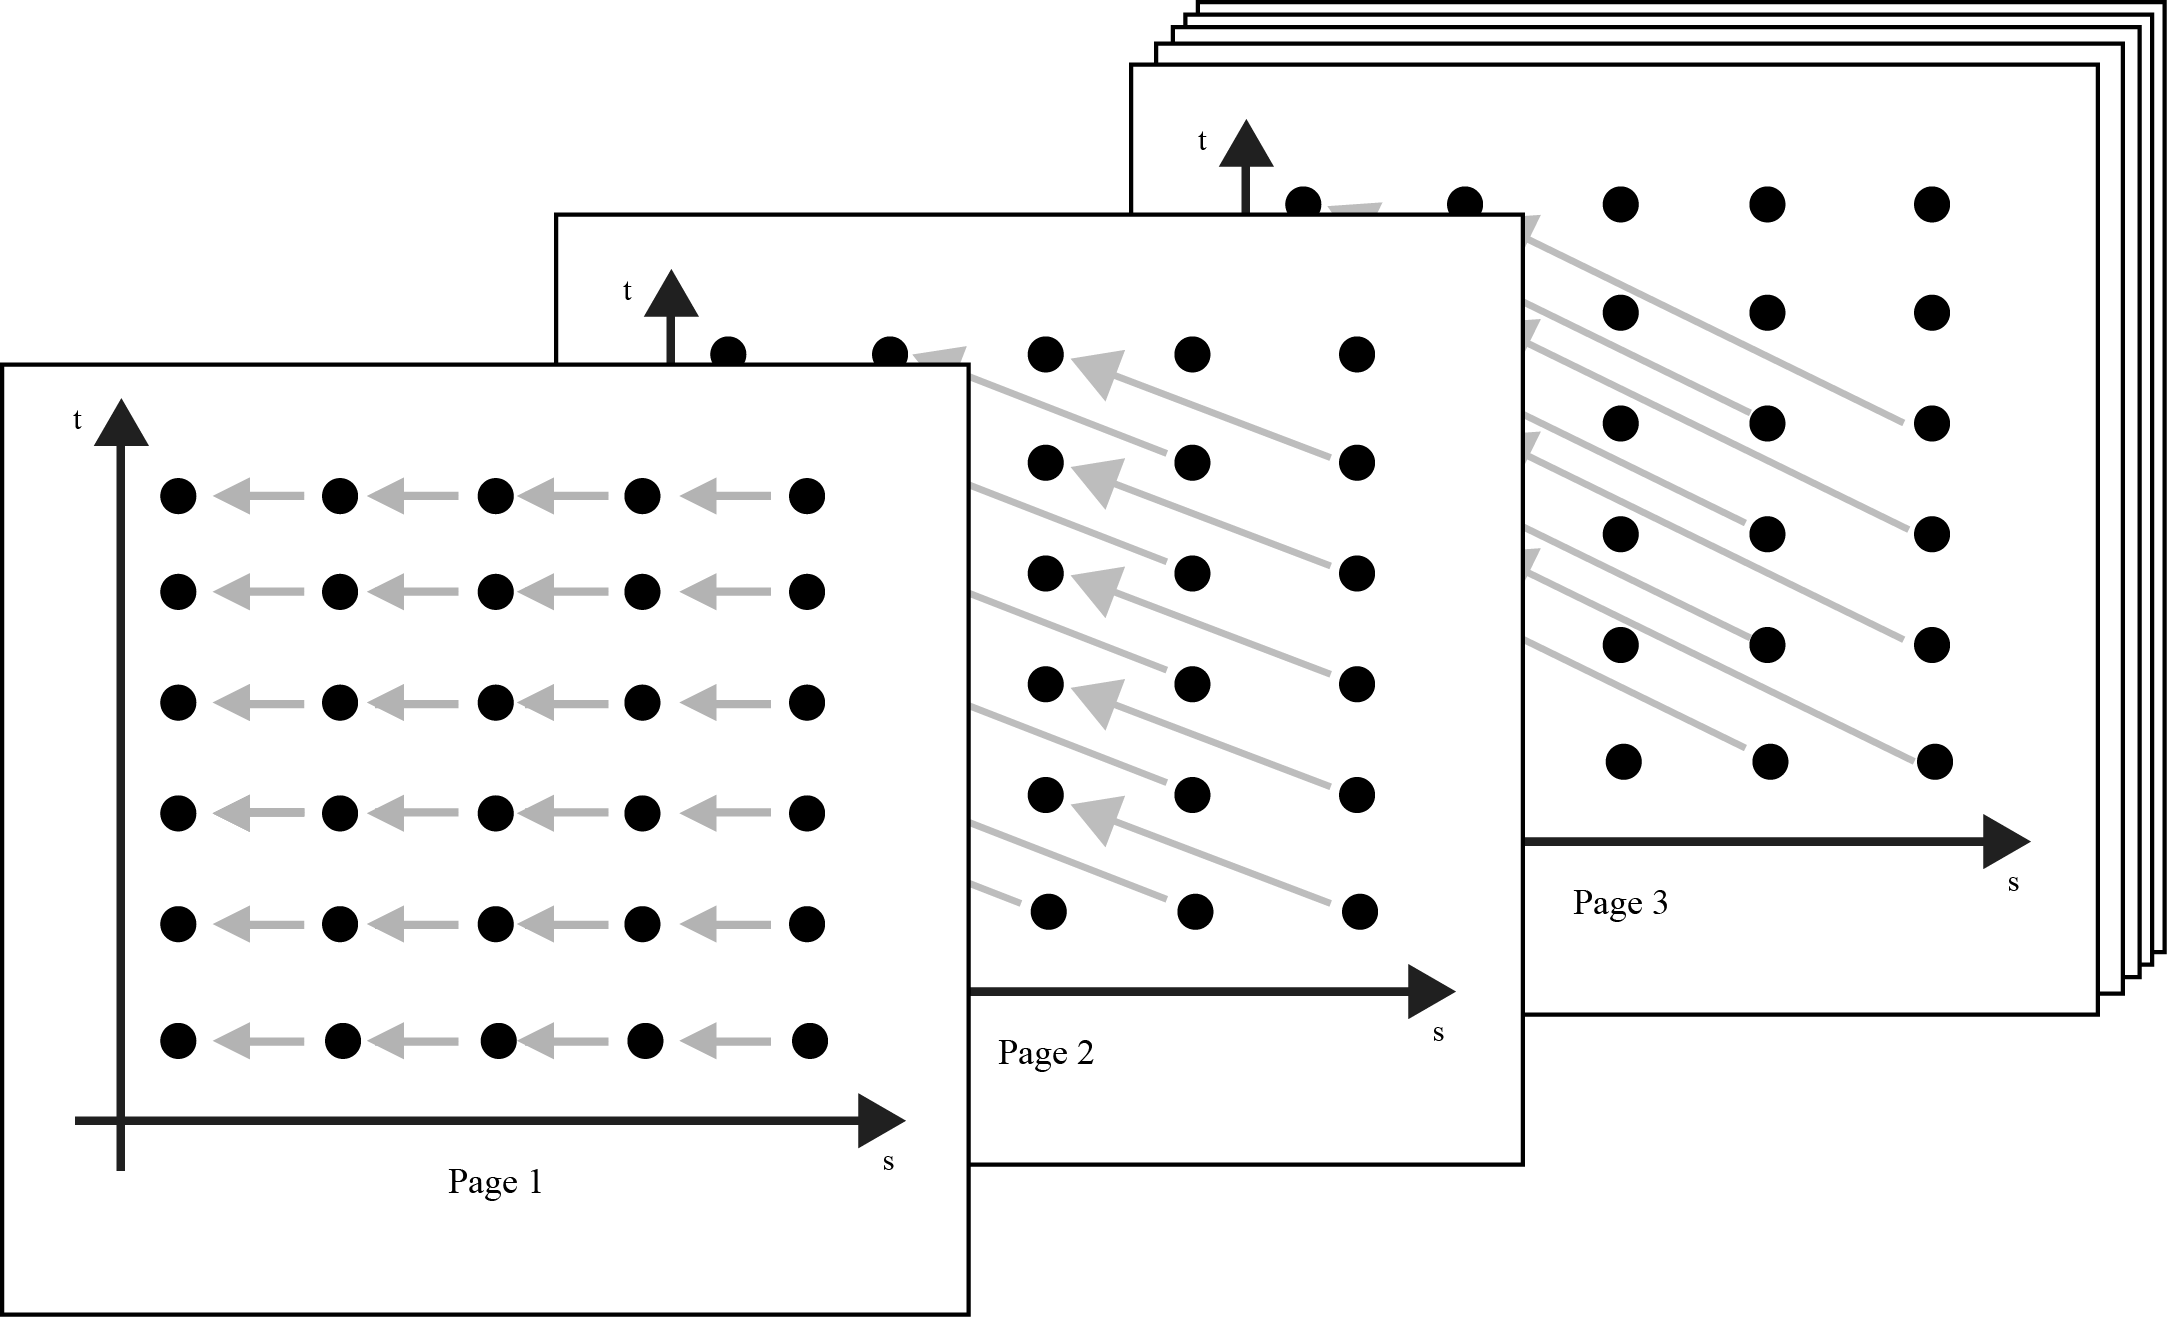
\includegraphics[width=\linewidth,height=0.5\textheight,keepaspectratio]{figures/cover.png}
  \end{center}
       \begin{minipage}{.35\linewidth}
    \begin{flushleft}
      \vspace{2em}
      {\fontsize{6pt}{2pt} \textit{Notes: These are notes live-tex'd
from a graduate course on Complex Analysis taught by Jingzhi Tie at the
University of Georgia in Spring 2020. As such, any errors or
inaccuracies are almost certainly my own. } } \\
    \end{flushleft}
    \end{minipage}
    \hfill
    \begin{minipage}{.65\linewidth}
    \end{minipage}
  }







\begin{document}

\date{}
\maketitle
\begin{flushleft}
\textbf{D. Zack Garza} \\
\textit{University of Georgia} \\
\textit{dzackgarza@gmail.com} \\
{\tiny \textit{Last updated:} 2020-10-25 }
\end{flushleft}


\newpage
\tableofcontents

\hypertarget{friday-january-10}{%
\section{Friday January 10}\label{friday-january-10}}

Recall that \(\CC\) is a field, where
\begin{align*}z = x + iy \implies \bar z = x - iy\end{align*} and if
\(z\neq 0\) then
\begin{align*}z\inv = \frac{\bar z} {\abs{z}^2}\end{align*}

\begin{description}
\tightlist
\item[Lemma (Triangle Inequality)]
\begin{align*}\abs{z + w} \leq \abs z + \abs w.\end{align*}
\item[Proof]
\begin{align*}
(\abs z + \abs w)^2 - \abs{z+w}^2 = 2( \abs{z\bar w} - \Re z\bar w ) \geq 0
.\end{align*}
\item[Lemma (Reverse Triangle Inequality)]
\begin{align*}\abs{\abs z - \abs w} \leq \abs{z-w}.\end{align*}
\item[Proof]
\begin{align*}
\abs z = \abs{z-w + w} \leq \abs{z-w} + \abs w \implies \abs w - \abs z \leq \abs{z-w} = \abs{w-z}
.\end{align*}
\item[Fact]
\((\CC, \abs{\wait})\) is a normed space.
\item[Definition (Limits of Complex Sequences)]
\begin{align*}\lim z_n = z \iff \abs{z_n - z} \to 0 \in \RR.\end{align*}
\item[Definition (Complex Discs)]
A \emph{disc} is defined as
\(D_r(z_0) \definedas \theset{z\in\CC \suchthat \abs{z-z_0} < r}\), and
a subset is open iff it contains a disc. By convention, \(D_r\) denotes
a disc about \(z_0 = 0\).
\item[Definition (Convergence in \(\CC\))]
\(\sum_k z_k\) \emph{converges} iff
\(S_N \definedas \sum_{\abs k < N} z_k\) converges.
\end{description}

Note that \(z_n \to z\) and \(z_n = x_n + iy_n\), and
\begin{align*}\abs{z_n - z} = \sqrt{(x_n - x)^2 - (y_n - y)^2} < \varepsilon \implies \abs{x - x_n}, \abs{y - y_n} < \varepsilon.\end{align*}

Since \(\RR\) is complete iff every Cauchy sequence converges iff every
bounded monotone sequence has a limit.

\begin{quote}
Note: This is useful precisely when you don't know the limiting term.
\end{quote}

Note that \(\sum_k z_k\) thus converges if
\(\abs{\sum_{k=m}^n z_k} < \varepsilon\) for \(m, n\) large enough, so
sums converges iff they have small tails.

\begin{description}
\tightlist
\item[Definition (Absolute Convergence)]
\(S_N = \sum^N z_k\) \emph{converges absolutely} iff
\(\tilde S \definedas \sum^N \abs{z_k}\) converges.
\end{description}

Note that the partial sums \(\sum^N \abs{z_k}\) are monotone, so
\(\tilde S_N\) converges iff the partial sums are bounded above.

\begin{description}
\tightlist
\item[Definition (Power Series)]
A sum of the form \(\sum_{k=0}^\infty a_k z_k\) is a \emph{power
series}.
\end{description}

\emph{Examples}:

\begin{align*}
\sum x^k &= \frac 1 {1-x} \\
\sum (-x^2)^k &= \frac 1 {1+x^2}
.\end{align*}

Note that both of these have a radius of convergence equal to 1, since
the first has a pole at \(x=1\) and the second as a pole at \(x = i\).

\hypertarget{monday-january-13th}{%
\section{Monday January 13th}\label{monday-january-13th}}

Recall that \(\sum z_k\) converges iff \(s_n = \sum_{k=1}^n z_k\)
converges.

\begin{description}
\tightlist
\item[Lemma]
Absolute convergence implies convergence.
\end{description}

The most interesting series: \(f(z) = \sum a_k z^k\), i.e.~power series.

\begin{description}
\tightlist
\item[Lemma (Divergence)]
If \(\sum z_k\) converges, then \(\lim z_k = 0\).
\item[Corollary]
If \(\sum z_k\) converges, \(\theset{z_k}\) is uniformly bounded by a
constant \(C > 0\), i.e.~\(\abs{z_k} < C\) for all \(k\).
\end{description}

\textbf{Proposition:} If \(\sum a_k z_k\) converges at some point
\(z_0\), then it converges for all \(\abs z < \abs z_0\).

Note that this inequality is necessarily strict. For example,
\(\sum \frac{z^{n-1}}{n}\) converges at \(z=-1\) (alternating harmonic
series) but not at \(z=1\) (harmonic series).

\begin{description}
\item[Proof]
Suppose \(\sum a_k z_1^k\) converges. The terms are uniformly bounded,
so \(\abs{a_k z_1^k} \leq C\) for all \(k\). Then we have
\begin{align*}\abs {a_k} \leq C/\abs{z_1}^k\end{align*}, so if
\(\abs z < \abs{z_1}\) we have
\begin{align*}\abs{a_k z^k} \leq \abs{z}^k \frac{C}{\abs{z_1}^k} = C (\abs{z} / \abs{z_1} )^k.\end{align*}
So if \(\abs{z} < \abs{z_1}\), the parenthesized quantity is less than
1, and the original series is bounded by a geometric series. Letting
\(r = \abs{z} / \abs{z_1}\), we have

\begin{align*}
\sum \abs{a_k z^k} \leq \sum c r^k = \frac{c}{1-r}
,\end{align*}

and so we have absolute convergence.
\item[Exercise (future problem set)]
Show that \(\sum \frac 1 k z^{k-1}\) converges for all \(\abs{z} = 1\)
except for \(z = 1\). (Use summation by parts.)
\item[Definition (Radius of Convergence)]
The \emph{radius of convergence} of a series is the real number \(R\)
such that \(f(z) = \sum a_k z^k\) converges precisely for \(\abs z < R\)
and diverges for \(\abs z > R\).

We denote a disc of radius \(R\) centered at zero by \(D_R\). If
\(R=\infty\), then \(f\) is said to be \emph{entire}.
\item[Proposition]
Suppose that \(\sum a_k z^k\) converges for all \(\abs{z} < R\). Then
\(f(z) = \sum a_k z^k\) is continuous on \(D_R\), i.e.~using the
sequential definition of continuity, \(\lim_{z\to z_0} f(z) = f(z_0)\)
for all \(z_0 \in D_R\).
\end{description}

Recall that \(S_n(z) \to S(z)\) uniformly on \(\Omega\) iff
\(\forall \varepsilon > 0\), there exists a \(M\in \NN\) such that
\begin{align*}n> M \implies \abs{S_n(z) - S(z)} < \varepsilon\end{align*}
for all \(z\in \Omega\)

Note that arbitrary limits of continuous functions may not be
continuous. Counterexample: \(f_n(x) = x^n\) on \([0, 1]\); then
\(f_n \to \delta(1)\). This uniformly converges on
\([0, 1-\varepsilon]\) for any \(\varepsilon > 0\).

\begin{description}
\item[Exercise]
Show that the uniform limit of continuous functions is continuous.

\begin{quote}
Hint: Use the triangle inequality.
\end{quote}
\item[Proof (of proposition)]
Write
\(f(z) = \sum_{k=0}^N a_k z^k + \sum_{N+1}^\infty a_k z^k \definedas S_N(z) + R_N(z)\).
Note that if \(\abs{z} < R\), then there exists a \(T\) such that
\(\abs{z} < T < R\) where \(f(z)\) converges uniformly on \(D_T\).

\begin{quote}
Check!
\end{quote}

We need to show that \(\abs{R_N(z)}\) is uniformly small for
\(\abs{z} < s < T\). Note that \(\sum a_k z^k\) converges on \(D_T\), so
we can find a \(C\) such that \(\abs{a_k z^k} \leq C\) for all \(k\).
Then \(\abs{a_k} \leq C/T^k\) for all \(k\), and so

\begin{align*}
\abs{\sum_{k=N+1}^\infty a_k z^k}
&\leq \sum_{k=N+1}^\infty \abs{a_k} \abs{z}^k \\
&\leq \sum_{k=N+1}^\infty  (c/T^k) s^k \\
&= c\sum \abs{s/T}^k \\
&= c \frac{r^{N+!}}{1-r}
&= C \varepsilon_n \to 0
,\end{align*}

which follows because \(0 < r = s/T < 1\).

So \(S_N(z) \to f(z)\) uniformly on \(\abs{z} < s\) and \(S_N(z)\) are
all continuous, so \(f(z)\) is continuous.
\end{description}

There are two ways to compute the radius of convergence:

\begin{itemize}
\tightlist
\item
  Root test: \(\lim_k \abs{a_k}^{1/k} = L \implies R = \frac 1 L\).
\item
\item
  Ratio test: \(\lim_k \abs{a_{k+1} / a_k} = L \implies R = \frac 1 L\).
\end{itemize}

As long as these series converge, we can compute derivatives and
integrals term-by-term, and they have the same radius of convergence.

\hypertarget{wednesday-january-15th}{%
\section{Wednesday January 15th}\label{wednesday-january-15th}}

\begin{quote}
See references: Taylor's Complex Analysis, Stein, Barry Simon (5 volume
set), Hormander (technically a PDEs book, but mostly analysis)
\end{quote}

\begin{quote}
Good Paper:
\href{https://projecteuclid.org/download/pdf_1/euclid.acta/1485892151}{Hormander
1955}
\end{quote}

We'll mostly be working from Simon Vol. 2A, most problems from from
Stein's Complex.

\hypertarget{topology-and-algebra-of-cc}{%
\subsection{\texorpdfstring{Topology and Algebra of
\(\CC\)}{Topology and Algebra of \textbackslash CC}}\label{topology-and-algebra-of-cc}}

To do analysis, we'll need the following notions:

\begin{enumerate}
\def\labelenumi{\arabic{enumi}.}
\item
  Continuity of a complex-valued function \(f: \Omega \to \Omega\)
\item
  Complex-differentiability: For \(\Omega \subset \CC\) open and
  \(z_0 \in \Omega\), there exists \(\varepsilon > 0\) such that
  \(D_\varepsilon = \theset{z \suchthat \abs{z - z_0} < \varepsilon} \subset \Omega\),
  and \(f\) is \textbf{holomorphic} (complex-differentiable) at \(z_0\)
  iff
  \begin{align*}\lim_{h\to 0} \frac 1 h (f(z_0 + h) - f(z_0))\end{align*}
  exists; if so we denote it by \(f'(z_0)\).
\end{enumerate}

\begin{description}
\item[Example]
\(f(z) = z\) is holomorphic, since \(f(z+ h) - f(z) = z+h-z = h\), so
\(f'(z_0) = \frac h h = 1\) for all \(z_0\).
\item[Example]
Given \(f(z) = \bar z\), we have \(f(z+h)-f(z) = \bar h\), so the ratio
is \(\frac{\bar h}{h}\) and the limit doesn't exist.

Note that if \(h\in \RR\), then \(\bar h = h\) and the ratio is
identically 1, while if \(h\) is purely imaginary, then \(\bar h = -h\)
and the limit is identically \(-1\).
\end{description}

We say \(f\) is \emph{holomorphic on an open set} \(\Omega\) iff it is
holomorphic at every point, and is holomorphic on a closed set \(C\) iff
there exists an open \(\Omega \supset C\) such that \(f\) is holomorphic
on \(\Omega\).

\begin{description}
\tightlist
\item[Fact]
If \(f\) is holomorphic, writing \(h = h_1 + ih_2\), then the following
two limits exist and are equal:
\end{description}

\begin{align*}
  \lim_{h_1 \to 0} \frac{f(x_0 + iy_0 + h_1) - f(x_0 + iy_0)}{h_1} = \dd{f}{x}(x_0, y_0) \\
  \lim_{h_2 \to 0} \frac{f(x_0 + iy_0 + ih_2) - f(x_0 + iy_0)}{ih_2} = \frac 1 i \dd{f}{y}(x_0, y_0) \\
  \implies \dd{f}{x} = \frac 1  i \dd{f}{y}
  .\end{align*}

So if we write \(f(z) = u(x, y) + i v(x, y)\), we have

\begin{align*}
  \dd{u}{x} + i \dd{v}{x} \mid_{(x_0, y_0)} = \frac 1 i \qty{
  \dd{u}{y} + i \dd{v}{y}
  } \mid_{(x_0, y_0)}
  ,\end{align*}

and equating real and imaginary parts yields \textbf{the Cauchy-Riemann
equations}:

\begin{align*}
  \dd{u}{x} + i \dd{v}{x} = -i \dd{u}{y} + \dd{v}{y} \\
  \iff \dd{u}{x} = \dd{v}{y} \quad\text{and}\quad \dd{u}{y} = - \dd{v}{x}
  .\end{align*}

The usual rules of derivatives apply:

\begin{enumerate}
\def\labelenumi{\arabic{enumi}.}
\tightlist
\item
  \((\sum f)' = \sum f'\)
\end{enumerate}

\begin{description}
\tightlist
\item[Proof]
Direct.
\end{description}

\begin{enumerate}
\def\labelenumi{\arabic{enumi}.}
\setcounter{enumi}{1}
\tightlist
\item
  \((\prod f)' =\) product rule
\end{enumerate}

\begin{description}
\tightlist
\item[Proof]
Consider \((f(z+h)g(z+h) - f(z)g(z))/h\) and use continuity of \(g\) at
\(z\).
\end{description}

\begin{enumerate}
\def\labelenumi{\arabic{enumi}.}
\setcounter{enumi}{2}
\tightlist
\item
  Quotient rule
\end{enumerate}

\begin{description}
\tightlist
\item[Proof]
Nice trick, write
\begin{align*}q = \frac f g\end{align*} so \(qg = f\), then
\(f' = q'g + qg'\) and \(q' = \frac {f'} g - \frac{fg'}{g^2}\).
\end{description}

\begin{enumerate}
\def\labelenumi{\arabic{enumi}.}
\setcounter{enumi}{3}
\tightlist
\item
  Chain rule
\end{enumerate}

\begin{description}
\item[Proof]
Use the fact that if \(f'(g(z)) = a\), then
\begin{align*}f(z+h) - f(z) = a h + r(z, h),\quad \abs{r(z, h)} = o(\abs h) \to 0.\end{align*}

Write \(b = g'(z)\), then
\begin{align*}f(g(z + h)) = f(g(z) + b h + r_1 ) = f(g(z)) + f'(g(z))bh + r_2\end{align*}
by considering error terms, and so
\begin{align*}\frac 1 h (f(g(z+h)) - f(g(z))) \to f'(g(z)) g'(z)\end{align*}.
\end{description}

\hypertarget{friday-january-17th}{%
\section{Friday January 17th}\label{friday-january-17th}}

\hypertarget{antiholomorphic-derivative}{%
\subsection{Antiholomorphic
Derivative}\label{antiholomorphic-derivative}}

\begin{quote}
Reference: See Lang's Complex Analysis, there are plenty of solution
manuals. Note: look for 13 statements equivalent to holomorphic:
Springer GTM Lipman.
\end{quote}

Let \(f; \Omega \to \CC\) be a complex-valued function. Recall that
\(f\) is \emph{complex differentiable} iff the usual ratio/limit exists.
Note that \(h = x+iy\) and \(h\to 0 \iff x,y\to 0\).

We can write
\begin{align*}f'(z) = \dd{f}{x} = \frac 1 i \dd{f}{y}.\end{align*} This
follows from Cauchy-Riemann since \(u_x = v_y\) and \(u_y = -v_x\).

We want to define \(\del, \bar \del\) operators. We have the identities

\begin{align*}
x = \frac{z + \bar z}{z} \quad y = \frac{z - \bar z}{iz}
.\end{align*}

We can then write

\begin{align*}
dz &= dx + idy \\
d\bar z &= dx - i dy
.\end{align*}

We define the dual operators by \(\inner{\dd{}{z}}{dz} = 1\) and
similarly \(\inner{ \dd{}{\bar z} }{d\bar z} = 1\).

By the chain rule, we can write

\begin{align*}
f_z &= \dd{f}{x} \dd{x}{z} +  \dd{f}{y} \dd{y}{z} \\
&= \frac 1 2 \dd{f}{x} + \dd{f}{y} \frac{1}{2i} \\
&= \frac 1 2 \qty{\dd{}{x} + i \dd{}{y} }f 
,\end{align*}

and similarly \begin{align*}
f_{\bar z} 
&=  \dd{f}{x} \dd{x}{\bar z}  + \dd{f}{y}  \dd{z}{\bar z} \\
&= \frac 1 2 \qty{ \dd{}{x} - \frac{1}{2i} \dd{}{y}  }f
.\end{align*}

We thus find \(\del_x = \del_z + \del_{\bar z}\) and
\(\del_y = i\qty{ \del_z - \del_{\bar z} }\), so define

\begin{align*}
\del f &\definedas \dd{f}{z} dz \\
\bar{\del} f &\definedas \dd{f}{\bar z} d\bar z \\
\implies df &= \dd{f}{z} dz + \dd{f}{\bar z} d\bar z
.\end{align*}

\begin{description}
\tightlist
\item[Definition (Holomorphic and Antiholomorphic Derivatives)]
\begin{align*}
\bd f &= \frac 1 2 \qty{\dd{}{x} + i \dd{}{y} }f\\
\bar \bd f &= \qty{ \dd{}{x} - \frac{1}{2i} \dd{}{y}  }f
.\end{align*}
\item[Proposition (Holomorphic Functions have vanishing antiholomorphic
derivatives)]
\(f\) is holomorphic iff \(\bar \del f = 0\).
\end{description}

This means that \(f\) depends on \(z\) alone and not \(\bar z\).

\begin{description}
\tightlist
\item[Proof]
\(\bar \del f = 0\) iff \(\frac 1 2 (f_x + if_y) = 0\), so
\((u_x - v_y) + i (v_x + u_y) = 0\).
\end{description}

Application to PDEs: we can write
\begin{align*}u_{xx} = v_{xy} \quad u_{yy} = v_{yx}\end{align*} and so
\begin{align*}u_{xx} + u_{yy} = 0 = v_{xx} + v_{yy}.\end{align*}

Thus \(\Delta f = 0\), sp \(f\) satisfies Laplace's equation and is said
to be \emph{harmonic}.

\begin{description}
\item[Corollary (Holomorphic Functions Have Harmonic Components)]
If \(f\) is analytic, then \(u, v\) are both harmonic functions.
\item[Theorem (Chain Rule)]
Let \(w = f(z)\) and \(g(w) = g(f(z))\). Then

\begin{align*}
h_z &= g_w f_z + g_{\bar w} \bar f_z \\
h_{\bar z} &= g_w f_{\bar z} + g_{\bar w} \bar f_{\bar z}
.\end{align*}

If \(f, g\) are holomorphic, \(f_{\bar z} = g_{\bar w} = 0\), so
\(h_{\bar z} = 0\) and \(h\) is holomorphic and
\begin{align*}h_z = g_w f_z.\end{align*}
\item[Example]
Given a power series \(f=\sum a_n (z- z_0)^n\). Then

\begin{enumerate}
\def\labelenumi{\arabic{enumi}.}
\tightlist
\item
  There exists a radius of convergence \(R\) such that \(f\) converges
  precisely on \(D_R(z_0)\).
\item
  \(f\) is continuous on \(D_R(z_0)^\circ\).
\item
  By the root test,
  \(R = (\limsup \abs{a_n}^{1/n})\inv = \liminf \abs{a_n/a_{n+1}} = (\limsup \abs{a_{k+1}/a_k})\inv\).
\end{enumerate}
\end{description}

Recall the \textbf{ratio test}:
\begin{align*}\sum \abs{a_k} <\infty \iff \limsup \abs{a_{k+1} / a_k} < 1\end{align*}

\begin{description}
\item[Theorem (Holomorphic series can be differentiated term-by-term)]
If \(f(z) = \sum_{n=0} a_n z^n\) is holomorphic on \(\abs{z} < R\) for
\(R> 0\) then
\begin{align*}f'(z) = \sum_{n=1} a_n n z^{n-1}.\end{align*}
\item[Proof]
Given \(\abs z < R\), fix \(r>0\) such that \(\abs {z} < r < R\).
Suppose that \(\abs{w-z} < r - \abs{z}\), so \(\abs w < r\).

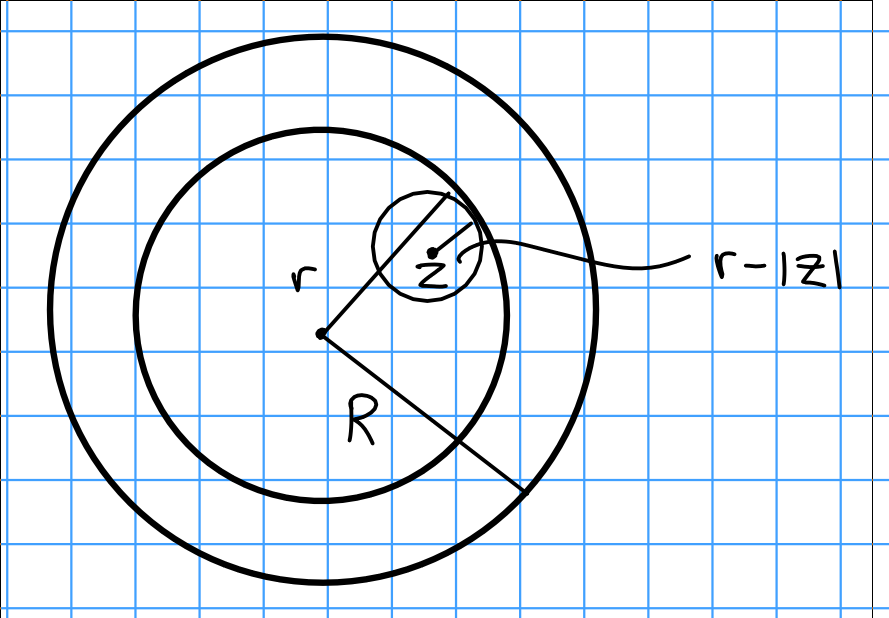
\includegraphics{figures/2020-01-17-14:14.png}\\

We want to show \begin{align*}
\abs{S} = \abs{\frac{f(w) - f(z)}{w - z} - \sum_{n=1} a_n n z^{n-1}} \to 0 \quad \text{as } w\to z
.\end{align*}

Idea: write everything in terms of power series. Use the fact that
\(a^n - b^n = (a-b)(a^{n-1} + a^{n-2}b + \cdots)\), and so
\(\abs{(w^k-z^k)/(w-z)} \leq k r^{k-1}\).

\begin{align*}
S 
&= \sum_{n=1} a_n \qty{ \frac{w^n - z^n}{w-z} - n z^{n-1}  } \\
&= \sum a_n \qty{ w^{n-1} + w^{n-2}z + \cdots + z^{n-1} + nz^{n-1} } \\
&=  \sum a_n \qty{ (w^{n-1} - z^{n-1}) + (w^{n-2} - z^{n-2})z + \cdots + (w-z) z^{n-2} }
&= \sum a_n (w-z) \qty{ \cdots + z^{n-2} }\\
&\leq \sum_{n=2} \abs{a_n} \frac 1 2 n(n-1) r^{n-2} \abs{z-w}
.\end{align*}
\item[Exercise]
Show \(\lim_n n^{\frac 1 n} = 1\).

Also tricky: show \(\lim \sin(n)\) doesn't exist, and \(\sin(n)\) is
dense in \([-1, 1]\).

\begin{description}
\tightlist
\item[Proof]
Consider \(\limsup \abs{a_n n}^{\frac 1 n}\).
\end{description}
\end{description}

Note that an analytic function is holomorphic in its domain of
convergence, so analytic implies holomorphic. The converse requires
Cauchy's integral formula.

Next time: trying to prove holomorphic functions are analytic.

\hypertarget{wednesday-january-22nd}{%
\section{Wednesday January 22nd}\label{wednesday-january-22nd}}

\hypertarget{parameterized-curves}{%
\subsection{Parameterized Curves}\label{parameterized-curves}}

\begin{quote}
Note: multiple complex variables, see Hormander or Steven Krantz
\end{quote}

Recall from last time that if
\begin{align*}f(z) = \sum_{n=0}^\infty a_n z^n\end{align*} with
\(z_0 \neq 0\) has radius of convergence
\begin{align*}R = (\limsup \abs{a_n}^{1/n})\inv > 0\end{align*} then
\(f'\) exists and is obtained by differentiating term-by-term.

We know that \(f\) analytic \(\implies\) \(f\) holomorphic (and smooth),
and we want to show the converse. For this, we need integration.

\begin{description}
\tightlist
\item[Definition (Parameterized Curves)]
A \emph{parameterized curve} is a function \(z(t)\) which maps a closed
interval \([a, b] \subset \RR\) to \(\CC\).
\item[Definition (Smooth Curves)]
The curve is said to be \emph{smooth} iff \(z'\) exists and is
continuous on \([a,b]\), and \(z'(t) \neq 0\) for any \(t\). At the
boundary \(\theset{a, b}\), we define the derivative by taking one-sided
limits.
\item[Definition (Piecewise Smooth Curves)]
A curve is said to be \emph{piecewise smooth} iff \(z(t)\) is continuous
on \([a, b]\) and there are \(a < a_1 < \cdots < a_n = b\) with \(z\)
smooth on each \([a_k, a_{k+1}]\).
\end{description}

Note that such a curve may fail to have tangent lines at \(a_i\).

\begin{description}
\tightlist
\item[Definition (Equivalent Parameterizations)]
Two parameterizations \(z: [a,b] \to \CC, \tilde z: [c, d] \to \CC\) are
\emph{equivalent} iff there exists a \(C^1\) bijection
\(s: [c, d] \to [a, b]\) where \(s \mapsto t(s)\) such that \(s'>0\) and
\(\tilde z(s) = z(s(t))\).
\end{description}

Note that \(s' > 0\) preserves orientation and \(s'<0\) reverses
orientation.

\begin{description}
\tightlist
\item[Definition (Orientations of Curves)]
A curve in \emph{reverse orientation} is defined by \begin{align*}
\gamma: [a, b] \to \CC \implies 
\gamma^-: [a,b] &\to \CC \\ t &\mapsto \gamma(a+b-t)
.\end{align*}
\item[Definition (Closed Curves)]
A curve is \emph{closed} iff \(z(a) = z(b)\), and is simple iff
\(z(t) \neq z_{t_1}\) for \(t\neq t_1\).
\item[Definition (Positively Oriented Curves)]
For \(C_r(z_0) \definedas \theset{z\suchthat \abs{z-z_0} = r}\), the
\emph{positive orientation} is given by \(z(t) = z_0 + re^{2\pi i t}\)
for \(t\in [0, 1]\).
\end{description}

\hypertarget{definition-of-the-integral}{%
\subsection{Definition of the
Integral}\label{definition-of-the-integral}}

\begin{description}
\item[Definition (The Complex Integral)]
The \emph{integral} of \(f\) over \(\gamma\) is defined as

\begin{align*}
\int_\gamma f ~dz = \int_a^b f(z(t)) z'(t)~dt
.\end{align*}
\end{description}

Note: this doesn't depend on parameterization, since if \(t = t(s)\),
then a change of variables yields \begin{align*}
\int_\gamma f ~dz - \int_c^d f(z(t(s)))~z'(t(s))~t'(s) ~ds = \int_c^d f(\tilde z(s)) ~\tilde z'(s) ~ds
.\end{align*}

\begin{description}
\item[Definition (Length of a Curve)]
The \emph{length} of \(\gamma\) is defined as
\(\abs \gamma = \int \abs{z'(t)} ~dt\).
\item[Proposition]
\begin{enumerate}
\def\labelenumi{\arabic{enumi}.}
\item
  We can extend this definition to piecewise smooth curves by
  \begin{align*}
  \int_\gamma f~dz = \sum \int_{a_k}^{a_{k+1}} f ~dz
  \end{align*}
\item
  This integral is linear and \(\int_\gamma f = -\int_{\gamma^-} f\).
\item
  We have an inequality
\end{enumerate}

\begin{align*}
\abs{\int_\gamma f} \leq \max_{a\leq t \leq b} \abs{f(z(t))} \abs\gamma
.\end{align*}
\item[Definition (Primitive of a Function)]
A function \(F\) is a \emph{primitive} for \(f\) on \(\Omega\) iff \(F\)
is holomorphic on \(\Omega\) and \(F'(z) = f(z)\) on \(\Omega\).
\end{description}

Recall that in \(\RR\), we have
\begin{align*}F(x) =\int_a^x f(t)~dt\end{align*} as an antiderivative
with \(F'(x) = f(x)\), and \(\int f = F(b) - F(a)\).

\begin{description}
\item[Theorem (Evaluating Integrals with Primitives)]
If \(f\) is continuous, has a primitive \(F\) in \(\Omega\), and
\(\gamma\) is a curve beginning at \(w_0\) and ending at \(w_1\), then
\(\int_\gamma f = F(w_1) - F(w_0)\).
\item[Proof]
Use definitions, write \(z(t)\) where \(z(a) = w_1, z(b) = w_2\). Then

\begin{align*}
\int_\gamma f &= \int_a^b f(z(t)) z'(t) ~ dt \\
&= \int_a^b F'(z(t)) z'(t) ~dt \\
&= \int_a^b F_t ~dt \\
&= F(z(b)) - F(z(a)) \quad\text{by FTC}\\
&= F(w_1) - F(w_2)
.\end{align*}

Note that if \(\gamma\) is piecewise smooth, the sum of the integrals
telescopes to yield the same conclusion.
\item[Corollary (Functions with Primitives Integrate to Zero Along
Loops)]
If \(f\) is continuous and \(\gamma\) is a closed curve in \(\Omega\),
and \(f\) has a primitive in \(\Omega\), then
\begin{align*}\oint f = 0.\end{align*}
\end{description}

\hypertarget{friday-january-24th}{%
\section{Friday January 24th}\label{friday-january-24th}}

\begin{description}
\item[Corollary]
If \(\gamma\) is a closed curve on \(\Omega\) an open set and \(f\) is
continuous with a primitive in \(\Omega\) (i.e.~an \(F\) holomorphic in
\(\Omega\) with \(F'=f\)) then \(\int_\gamma f ~dz = 0\).
\item[Proof (easy)]
\begin{align*}
\int_\gamma f ~dz = \int_\gamma F' = F'(z) z(t) ~dt  = F(z(b)) - F(z(a)) = 0
.\end{align*}
\item[Corollary]
If \(f\) is holomorphic with \(f'=0\) on \(\Omega\), then \(f\) is
constant.
\item[Proof (easy)]
Pick \(w_0 \in \Omega\); we want to fix \(w_0 \in \Omega\) and show
\(f(w) = f(w_0)\) for all \(w\in \Omega\).

Take any path \(\gamma: w_0 \to w\), then

\begin{align*}
0 = \int_\gamma f' = f(w) - f(w_0)
.\end{align*}
\end{description}

\hypertarget{integral-and-fourier-transform-of-e-x2}{%
\subsection{\texorpdfstring{Integral and Fourier Transform of
\(e^{-x^2}\)}{Integral and Fourier Transform of e\^{}\{-x\^{}2\}}}\label{integral-and-fourier-transform-of-e-x2}}

\begin{description}
\item[Example]
Let \(f(z) = e^{-z^2}\), this is holomorphic. Write
\begin{align*}
f(z) = \sum  \frac{(-1)^nz^{2n}}{n!}
,\end{align*} so
\begin{align*}
\int f = \sum  \frac{ (-1)^n z^{2n+1} }{ n! (2n+1) }
.\end{align*}

Since \(f\) is entire, \(\int f\) is entire, and \((\int f)' = f\) so
this function has a primitive. Thus \(\int_\gamma f(z) = 0\) for
\emph{any} closed curve. So take \(\gamma\) a rectangle with vertices
\(\pm a , \pm a + ib\).

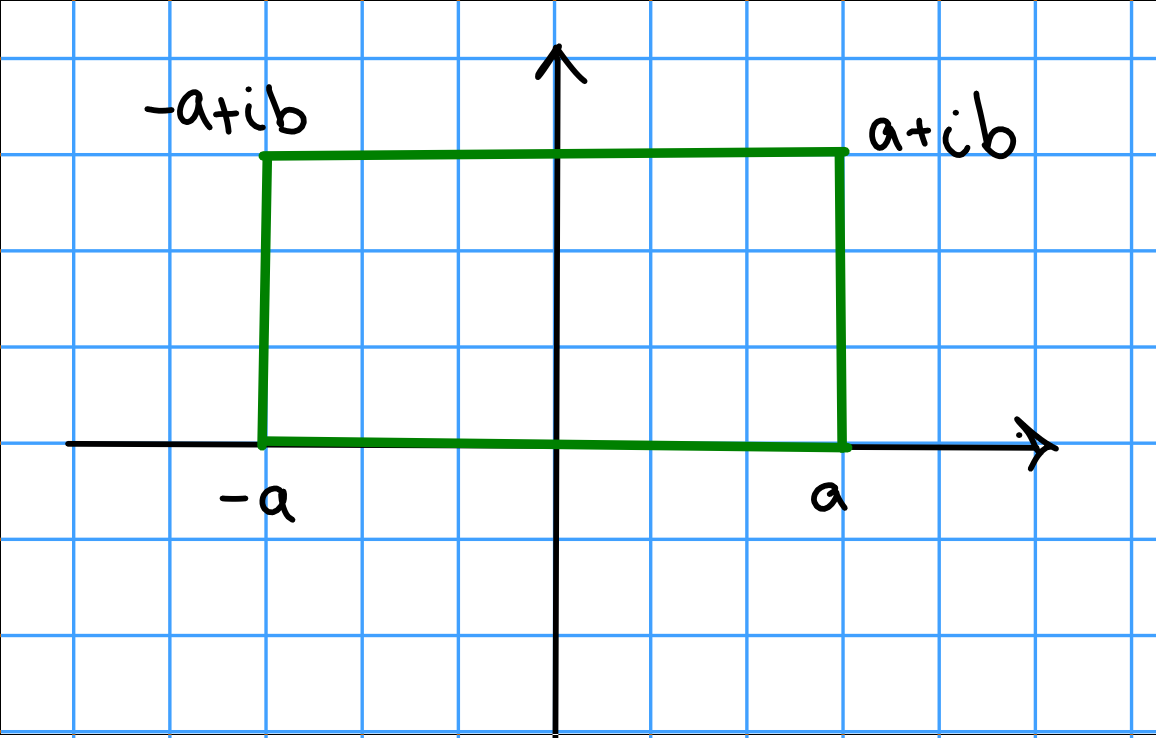
\includegraphics{figures/2020-01-24-13:36.png}\\

So

\begin{align*}
\int_\gamma f = \int_{-a}^a e^{-x^2} ~dx + \int e^{-(a+iy)^2} i ~dy - \int_{-a}^a e^{-(x+ib)^2} ~dx - \int_0^b e^{-(a+iy)^2} i dy = 0
.\end{align*}

We can do some estimates,

\begin{align*}
e^{-(a+iy)^2} 
&= e^{-(a^2 + 2iay - y^2)} \\
&= e^{-a^2 + y^2} e^{2iay} \\
&\leq e^{-a^2 + y^2} \\
&\leq e^{-a^2 + b^2}, \\ \\
\abs {\int_0^b e^{-(a+ib)^2} i ~dy} 
&\leq e^{-a^2 + b^2} \cdot b \\ \\
\int_{-a}^a e^{-(x^2 + 2ib x)-b^2} 
&= e^{b^2} \int_{-a}^a e^{-x^2} ( \cos(2bx) - i \sin(2bx) ) \\ \\
&\equalsbecause{odd fn} e^{b^2} \int_{-a}^a e^{-x^2} \cos(2bx) ~dx
.\end{align*}

Now take \(a\to \infty\) to obtain

\begin{align*}
\int_\RR e^{-x^2} ~dx = e^{b^2} \int_\RR e^{-x^2} \cos(2bx) ~dx
.\end{align*}

We can compute

\begin{align*}
\int_\RR e^{-x^2} = \left[ \qty{\int_\RR e^{-x^2}}^2 \right]^{1/2} = \qty{ \int_0^{2\pi} \int_0^\infty e^{r^2} r~dr~d\theta} = \sqrt{\pi}
.\end{align*}

and then conclude

\begin{align*}
\int_\RR e^{-x^2} \cos(2bx) = \sqrt{\pi} e^{-b^2}
.\end{align*}

Make a change of variables \(2b = 2\pi \xi\), so \(b = \pi \xi\), then

\begin{align*}
\int_\RR e^{-x^2} \cos(2\pi \xi x) ~dx = \sqrt{\pi} e^{-\pi^2 \xi^2}
.\end{align*}

Thus \(\mcf(e^{-x^2}) = \sqrt{\pi} e^{-\pi^2 \xi^2}\), allowing
computation of the Fourier transform. Note that this can be used to
prove the Fourier inversion formula.
\item[Exercise]
Show that this is an approximate identity and prove the Fourier
inversion formula.
\item[Exercise]
Show \(\mcf(e^{-ax^2}) = \sqrt{\pi/a} e^{-\pi^2/a \cdot \xi^2}\), and
thus taking \(a = \pi\) makes \(e^{\pi x^2}\) is an eigenfunction of
\(\mcf\) with eigenvalue \(1\).
\item[Theorem (Holomorphic Integrals Vanish)]
If \(f\) has a primitive on \(\Omega\) then \(F(z)\) is holomorphic and
\(\int_\gamma f = 0\). If \(f\) is holomorphic, then
\begin{align*}\int_\gamma f = 0.\end{align*}
\item[Theorem (Green's)]
Take \(\Omega \in \RR^2\) bounded with \(\bd \Omega\) piecewise smooth.
If \(f, g\in C^1{\bar \Omega}\), then

\begin{align*}
\int_{\bd \Omega} f ~dx + g ~dy = \iint_{\Omega} \qty{g_x - f_y} ~dA
.\end{align*}
\item[Proof]
Omitted.
\item[Proof (that holomorphic integrals vanish)]
Write \(\gamma = \bd \Gamma\), and noting that
\(f_z = f_x = \frac 1 i f_y\) implies that \(\dd{f}{\bar z}\), so

\begin{align*}
\int_\gamma f ~dz 
&= \int_\gamma f(z) ~(dx + i dy) \\
&= \int f(z) ~dx + i f(z) ~dy \\
&= \iint_\Gamma \qty{if_x - f_y} ~dA \\
&= i \iint_\Gamma \qty{f_x - \frac 1 i f_y} ~dA \\
&= i \iint 0 ~dA \\
&= 0
.\end{align*}
\end{description}

Next up, we'll prove that this integral over any triangle is zero by a
limiting process.

\hypertarget{monday-january-27th}{%
\section{Monday January 27th}\label{monday-january-27th}}

\begin{quote}
Open question: does a PDE involving analytic functions always have
solutions? Or does this hold with analytic replaced by smooth?
\end{quote}

\hypertarget{greens-theorem}{%
\subsection{Green's Theorem}\label{greens-theorem}}

Fix a connected domain \(\Omega\) which is bounded with a piecewise
\(C^1\) boundary.

\begin{description}
\item[Theorem (Green's)]
Given \(f, g \in C^1 \bar \Omega\), we can take a vector field
\(F = \generators{f, g}\) and have

\begin{align*}
\int_{\bd \Omega} f~dx + g~dy &= \iint_{\Omega} \qty{ \dd{g}{x} - \dd{f}{y}  } ~dA \\
\int_{\bd \Omega} - f~dx + g~dy &= \iint_{\Omega} \qty{ \dd{g}{x} + \dd{f}{y}  } ~dA \\
\int_{\bd \Omega} f~dy - g~dy &= \iint_{\Omega} \qty{ \dd{f}{x} + \dd{g}{y}  } ~dA \\
\int_{\bd \Omega} F \cdot \vector n ~ds &= \iint_{\Omega} \nabla \cdot F ~dA \\
\int_{\bd \Omega} \mathrm{curl}(F) ~ds &= \iint_{\Omega} \mathrm{div}(F) ~dA
,\end{align*}

where we take \(\vector n\) to be orthogonal to \(\bd \Omega\). The
quantities appearing on the RHS are referred to as the flux.
\end{description}

For \(f(z) \in C^1(\Omega)\) holomorphic, we can then write

\begin{align*}
\int_{\bd \Omega} f ~dz
&= \int_{\bd \Omega} f ~(dx + idy) \\
&= \int_{\bd \Omega} f ~dx + if~dy \\
&= \iint_\Omega \qty{if_x - f_y} ~dA \\
&= 0
,\end{align*}

which follows since \(f\) holomorphic, we can write
\begin{align*}f'(z) = f_x = \frac 1 i f_y,\end{align*} so
\(i f_x = f_y\) and thus \(\dd{f}{\bar z} = 0\).

\begin{quote}
See Taylor's Introduction to Complex Analysis
\end{quote}

\begin{description}
\item[Theorem (Cauchy's Integral Formula):]
If \(f\in C^1(\bar \Omega)\) and \(f\) is holomorphic, then for any
\(z\in \Omega\)

\begin{align*}
f(z) = \frac{1}{2\pi i} \int_{\bd \Omega} \frac{d(\xi)}{\xi - z} ~d\xi
.\end{align*}
\item[Proof]
Since \(z\in \Omega\) an open set, we can find some \(r> 0\) such that
\(D_r(z) \subset \Omega\). Then \(\frac{f(\xi)}{\xi - z}\) is
holomorphic on \(\Omega\setminus D_r(z)\). Let \(C_r = \bd D_r(z)\).

\textbf{Claim}:
\begin{align*}\int_{\bd \Omega} \frac{f(\xi)}{\xi - z} ~d\xi = \int_{C_r} \frac{f(\xi)}{\xi - z} ~ d\xi.\end{align*}

If we can differentiate through the integral, we can obtain

\begin{align*}
\dd{}{z} f(z) = \frac 1 {2\pi i} \int_{\bd \Omega} \frac{f(\xi)}{(\xi - z)^2} ~d\xi
.\end{align*}

and thus inductively

\begin{align*}
(D_z)^n f(z) = \frac{n!}{2\pi i} \int_{\bd \Omega} \frac{ f(\xi) ~d\xi  }{ (\xi - z)^{n+1}  }
.\end{align*}

To prove rigorously, need to write

\begin{align*}
\Delta_h f(z) 
= \frac 1 h \qty{ f(z+h) - f(z) } \\
= \frac 1 {2\pi i h} \int_{\bd \Omega} f(\xi) \qty{ \frac{1}{\xi - (z+h)} - \frac{1}{\xi - z}  } ~d\xi
= \frac 1 {2\pi i h} \int_{\bd \Omega} f(\xi) \qty{ \frac{1}{ (\xi - z- h)(\xi - z)  }  } ~d\xi
,\end{align*}

and show the integrand converges uniformly, where
\begin{align*}
\frac{1}{(\xi - z - h)(\xi - z)} \converges{u}\to \frac{1}{(\xi - z)^2}
.\end{align*}

Continuing inductively yields the integral formula.
\item[Proof (of claim used in main proof)]
Use the parameterization of \(C_r\) given by \(\xi = z + re^{i\theta}\).
Then

\begin{align*}
\frac{1}{2\pi i} \int_{C_r} \frac{f(\xi)}{\xi - z} ~d\xi 
&= \frac{1}{2\pi i} \int_0^{2\pi} \frac{f(z + re^{i\theta})}{re^{i\theta}} ~ird\theta \\
&= \frac{1}{2\pi} \int_0^{2\pi} f(z + re^{i\theta}) ~d\theta \\
&\converges{r \to 0}\to \frac{1}{2\pi} \int_{\bd \Omega} \frac{f(\xi)} {\xi - z}
.\end{align*}

where we use the fact that
\begin{align*}f(z + re^{i\theta}) = f(z) + f'(z)re^{i\theta} + o(r) \converges{r\to 0}\to f(z)\end{align*}

Letting
\begin{align*}F(\xi) = \frac{ f(\xi)}{\xi - z},\end{align*} this is
holomorphic on \(\Omega\setminus D_r(z)\). Let
\(\Omega_r = \bd \Omega \union (-C_r)\). Take the following path
integral:

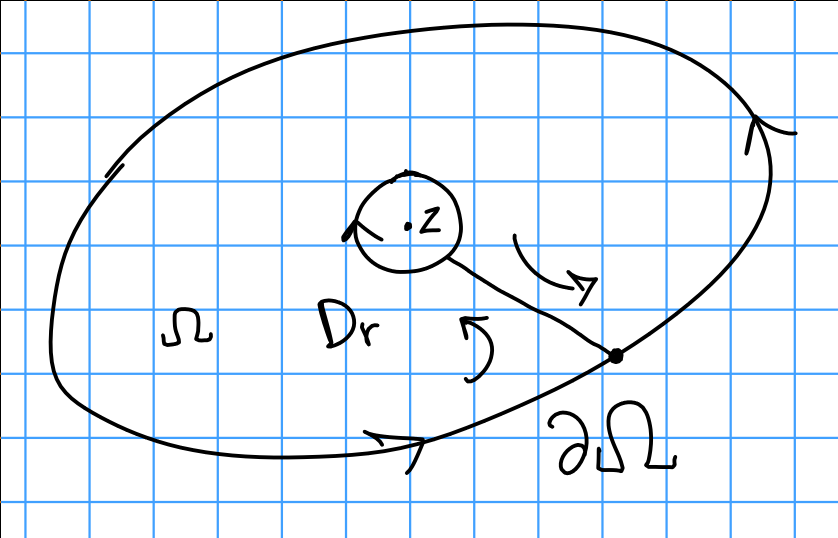
\includegraphics{figures/2020-01-27-13:59.png}\\

Then \begin{align*}
0 = \int_{\bd \Omega_r} F(\xi) ~d\xi = \int_{\bd \Omega} F(\xi) ~d\xi - \int_{C_r} F(\xi) ~d\xi
,\end{align*}

which forces these integrals to be equal.
\item[Corollary (\(C^1\) implies smooth)]
If \(f\) is holomorphic, then \(f\in C^1(\Omega)\) implies that
\(f \in C^\infty(\Omega)\).
\item[Theorem (Holomorphic implies analytic)]
If \(f\) is holomorphic in \(\Omega\), then \(f\) is equal to its Taylor
series (i.e.~\(f(z_0\) is analytic.)
\item[Proof]
Fix \(z_0 \in \Omega\) and let \(r = \abs{z- z_0}\).

\begin{align*}
\frac{1}{\xi - z} 
&= \frac{1}{ \xi - z_0 - (z-z_0)  } \\
&= \frac{1}{\xi - z_0} \frac{1}{1 - \qty{ \frac{z-z_0}{\xi - z_0}   }  } \\
&= \frac{1}{\xi - z_0} \sum_n \qty{ \frac{z - z_0}{\xi - z_0}  }^n \quad\text{for } \abs{z - z_0} < \abs{\xi - z_0}
.\end{align*}

Note that \(\sum z^n\) converges uniformly for any
\(\abs{z} < \delta < 1\).

Thus

\begin{align*}
f(z) 
&= \frac{1}{2\pi i} \int_{\xi \in \bd\Omega} f(\xi) \sum \frac{(z-z_0)^n}{(\xi - z_0)^{n+1}} ~d\xi \\
&= \sum \qty{ \frac {1}{2\pi i} \int \frac{f(\xi)  }{(\xi - z_0)^{n+1}} ~d\xi} (z-z_0)^n \\
&= \sum \frac{f^{(n)} (z_0)}{n!} (z-z_0)^n
.\end{align*}
\item[Corollary]
\(f\) is holomorphic iff \(f\) is analytic.
\end{description}

Counterexample to keep in mind:

\begin{align*}
f(x) = \begin{cases}
x^2 & x > 0 \\
0 & x\leq 0
\end{cases}
.\end{align*}

In the case of \(\RR\), smooth and analytic are very different
categories of functions.

\hypertarget{wednesday-january-29th}{%
\section{Wednesday January 29th}\label{wednesday-january-29th}}

\hypertarget{cauchys-integral-formula}{%
\subsection{Cauchy's Integral Formula}\label{cauchys-integral-formula}}

\begin{description}
\item[Theorem (Cauchy's Integral Formula)]
Let \(f: \Omega \to \CC\) be holomorphic, so \(f\in C^1(\bar \Omega)\).
Then for any \(z\in \Omega\),

\begin{align*}
f(z) = \frac{1}{2\pi i} \int_{\bd \Omega} \frac{f(\xi)}{\xi - z} ~d\xi
.\end{align*}

In general, \begin{align*}
f^{(n)}(z) = \frac{n!}{2\pi i} \int_{\bd \Omega} \frac{f(\xi)}{\qty{\xi - z}^{n+1}} ~d\xi
.\end{align*}
\end{description}

This implies that \(f\) is analytic, i.e.~
\begin{align*}
f(z) = \sum a_n (z-z_0)^n \quad\text{where}\quad a_n = \frac{f^{(n)}(z_0) }{n!}
.\end{align*} Thus \(f\) is holomorphic iff \(f\) is analytic,

and

\begin{align*}
\int_{\bd \Omega} f = 0 \implies \int_{\bd \Omega_\gamma} \frac{f(\xi)}{\xi - z}~d\xi = 0
.\end{align*}

where \(\Omega_r = \Omega\setminus D_r(z)\), and
\(\bd \Omega_r = \bd \Omega \union (-\bd D_r)\).

We can thus shrink integrals:

\begin{align*}
\int_{\bd \Omega} \frac{f(\xi)} {\xi - z} ~d\xi = \int_{C_r} \frac{f(\xi)} {\xi - z} ~d\xi
.\end{align*}

\begin{description}
\item[Proposition (Homotopy Invariance)]
Let \(f\in C^1(\Omega)\) be holomorphic on \(\Omega\). Let
\(\gamma_s(t)\) be a family of smooth curves in \(\Omega\); then
\(\int_{\gamma_s} f\) is independent of \(s\).
\item[Proof]
Write
\begin{align*}\gamma_s(t) = \gamma(s, t): [a, b] \cross [0, 1] \to \Omega.\end{align*}

We have \(\gamma_s(0) = \gamma_s(1)\) so
\(\dd{\gamma}{s}(s, 0) = \dd{\gamma}{s}(s, 1)\). Then

\begin{align*}
\dd{\gamma}{s} 
&= \int_0^1 \qty{ f'(r(s, t)) \dd{r}{s} \dd{r}{t} + f(r(s, t)) \frac{\partial^2 \gamma}{\partial s \partial t} } ~dt \\
&= \int_0^1 \qty{ f'(r(s, t)) \dd{r}{s} \dd{r}{t} + f(r(s, t)) \frac{\partial^2 \gamma}{\partial \mathbf{t} \partial \mathbf{s}} } ~dt \\
&= \int_0^1 \dd{}{t} \qty{ f(\gamma(s, t))  \gamma_s } \\
&= f(\gamma(s, 1))\gamma_s(s, 1) - f(\gamma(s, 0)) \gamma_s(s, 0) \\
&= 0
.\end{align*}

where we can just take the paths \(\gamma(s, t) = z_0 \in \Omega\) for
all \(s, t\).
\item[Proposition (Pointwise Limit of Locally Uniform is Locally
Uniform)]
Let \(\Omega \subset \CC\) be open and \(f_v: \Omega \to \CC\). Suppose
that each \(f_v\) is holomorphic, \(f_v \to f\) pointwise, and
\emph{locally uniform}, i.e.~\(f_v \to f\) uniformly on every compact
\(K \subset \Omega\). Then \(f\) is holomorphic in \(\Omega\) and \(f\)
is locally uniform.
\item[Proof]
Given a compact set \(K \subset \Omega\), pick an \(O\) with smooth
boundary such that \(K \subset O \subset \bar O \subset \Omega\). We
have

\begin{align*}
f_v(z) &= \frac{1}{2\pi i} \int_{\bd O} \frac{f_v(\xi)}{\xi - z}~d\xi \\
f_v^{(n)}(z) &= \frac{n!}{2\pi i} \int_{\bd O} \frac{f_v(\xi)}{\qty{ \xi - z}^{n+1} }~d\xi \\
.\end{align*}

Then on \(\bd O\), we have uniform convergence

\begin{align*}
\frac{f_v(\xi)}{\qty{\xi - z}^{n+1}} \converges{u}\to
\frac{f(\xi)}{\qty{\xi - z}^{n+1}}
.\end{align*}

By moving the limits inside, we obtain

\begin{align*}
f(z) &= \frac{1}{2\pi i} \int_{\bd O} \frac{f(\xi)}{\xi - z}~d\xi \\
f^{(n)}(z) &= \frac{n!}{2\pi i} \int_{\bd O} \frac{f(\xi)}{\qty{ \xi - z}^{n+1} }~d\xi \\
.\end{align*}
\item[Theorem (Cauchy's Inequality)]
Given \(z_0\in \Omega\), pick the largest disc
\(D_R(z_0) \subset \Omega\) and let \(C_R = \bd D_R\). Using the
integral formula, defining
\(\norm{f}_{C_R} = \max_{\abs{z-z_0} = R} \abs{f(z)}\)

\begin{align*}
\abs{ f^{(n)}(z_0) } \leq \frac{n!}{2\pi} \int_0^{2\pi} \frac{\norm{f}_{C_R}}{R^{n+1}} R~d\theta = \frac{n! \norm{f}_{C_R}}{R^{n}}
.\end{align*}
\item[Corollary (Liouville's Theorem)]
If \(f\) is entire and bounded, then \(f\) is constant.
\item[Proof]
For all \(z_0 \in \CC\), there exists an \(M\) such that
\(\abs{f(z)} \leq M\). Then \(\abs{f'(z_0)} \leq \frac{M}{R}\) for any
\(R> 0\). Taking \(R\to \infty\) yields \(f'(z_0) = 0\), so \(f\) is
constant.
\item[Corollary (Weak Fundamental Theorem of Algebra)]
Every non-constant polynomial \(p(z) = a_0 + a_1z + \cdots a_n z^n\) has
a root in \(\CC\).
\end{description}

Remark: A general proof technique is when proving something for
\(f(z)\), consider \(\frac{1}{f(z)}\) and \(f(\frac 1 z)\).

\begin{description}
\item[Proof]
Suppose \(p\) is nonconstant and does not have a root, \(\frac 1 p\) is
entire. Assume that \(a_n \neq 0\), then

\begin{align*}
\frac{p(z)}{z^n} = a_n \qty{ \frac{a_{n-1}}{z} + \cdots + \frac{a_0}{z^n}  } \definedas a_n + y
\end{align*}

We can note that \(\lim_{z\to \infty} \frac{a_{n-k}}{z^k} \to 0\), so
there exists an \(R>0\) such that

\begin{align*}
\abs{ \frac{p(z)}{z^n}  } \geq \frac 1 2 \abs{a_n} \quad \text{ for } \abs{z} > R \\
\implies \abs{p(z)} \geq \frac 1 2 \abs{a_n} \abs{z}^n \geq \frac 1 2 \abs{a_n} R^n
.\end{align*}

Since \(p(z)\) is continuous and has no root in the disc
\(\abs{z} \leq R\), \(\abs{p(z)}\) is bounded from below in this disc.
Since \(p(z)\) is continuous on a compact set, it attains a minimum, and
so \(\abs{p(z)} \geq \min_{\abs z \leq R} \abs{p(z)} = c_2 \neq 0\).
Then \(\abs{p(z)} \geq A = \min(C_2, \frac 1 2 \abs{a_n}R^n)\), so
\(\frac{1}{p}\) is bounded. Then \(f\) is constant, a contradiction.
\end{description}

\hypertarget{friday-january-31st}{%
\section{Friday January 31st}\label{friday-january-31st}}

\hypertarget{fundamental-theorem-of-algebra}{%
\subsection{Fundamental Theorem of
Algebra}\label{fundamental-theorem-of-algebra}}

Recall that if \(f\) is holomorphic, we have Cauchy's integral formula.

\begin{description}
\item[Corollary (Weak Fundamental Theorem of Algebra)]
If \(P(z)\) is a polynomial in \(\CC\) then \(P\) has a root in \(\CC\).
\item[Proof]
See previous notes.
\item[Corollary (Fundamental Theorem of Algebra)]
Every polynomial of degree \(n\) has precisely \(n\) roots in \(\CC\).
\item[Proof]
By induction on the degree of \(P\). From the first corollary, \(P\) has
a root \(w_1\), so write \(z = z-w_1 + w_1\). Then

\begin{align*}
p(z) 
&= p(z - w_1 + w_1) \\
&= \sum_k^n a_k(z -w_1 + w_1)^k \\
&= \sum_k^n a_k \sum_{j}^k {k\choose j} w_1{k-j} (z-w_1)^j \\
&= \sum_k^n \sum_j^k a_k {k\choose j} w_1^{k-j} (z-w_1)^j \\
&= \sum_j^n \qty{\sum_{k\geq j} a_k {k\choose j}}(z-w_1)^j \\
&= b_0 + b_1(z-w_1) + \cdots + b_n(z-w_1)^n 
.\end{align*}

Since \(P(w_1) = 0\), we must have \(b_0 = 0\), and thus this equals

\begin{align*}
b_1(z-w_1) + \cdots + b_n(z-w_1)^n 
&= (z-w_1) \qty{ b_1 + \cdots + b_n (z-w_1)^{n-1}  } \\
&\definedas  (z-w_1) \phi(z)
,\end{align*}

where \(\phi(z)\) is degree \(n-1\), which has \(n-1\) roots by
induction.
\item[Definition (Characterizations of Limit Points)]
For a sequence \(\theset{z_n}\), TFAE

\begin{enumerate}
\def\labelenumi{\arabic{enumi}.}
\tightlist
\item
  \(z\) is a limit point.
\item
  There exists a subsequence \(\theset{z_{n_k}}\) converging to \(z\).
\item
  For every \(\eps > 0\), there are infinitely many \(z_i\) in
  \(D_\eps(z)\).
\end{enumerate}
\item[Theorem (Only the zero function vanishes on a sequence in a domain
(Stein 4.8))]
Suppose \(f\) is holomorphic on a bounded connected region \(\Omega\)
and \(f\) vanishes on a sequence of distinct points with a limit point
in \(\Omega\). Then \(f\) is identically zero.
\item[Proof]
WLOG by restricting to a subsequence, suppose that
\(\theset{w_k} \in \Omega\) with \(f(w_i) = 0\) for all \(i\) and
\(z_0\) is a limit point of \(\theset{w_i}\). Let
\(U = \theset{ z\in \Omega \suchthat f(z) = 0 }\). Then

\begin{enumerate}
\def\labelenumi{\arabic{enumi}.}
\tightlist
\item
  \(U\) is nonempty since \(f(w_k) = f(z_0) = 0\).
\item
  Since holomorphic functions are continuous, if \(w_k \to z\) then
  \(z\in U\), so \(U\) is closed.
\item
  (To prove) \(U\) is open.
\end{enumerate}

Since \(U\) is closed and open, \(U = \Omega\).

We will first show that \(f(z) \equiv 0\) in a disk containing \(z_0\).
Choose a disc \(D\) containing \(z_0\) and contained in \(\Omega\).
Since \(f\) is holomorphic on \(D\), we can write
\begin{align*}f(z) = \sum a_nn (z-z_0)^n.\end{align*} Since
\(f(z_0) = 0\), we have \(a_0 = 0\).

Suppose \(f\not\equiv 0\). Then there exists a smallest \(n\in \ZZ^+\)
such that \(a_n \neq 0\), so \(f(z) = a_n(z-z_0)^n + \cdots\). Since
\(a_n \neq 0\), we can factor this as
\(a_n(z-z_0)^n \qty{ 1 + g(z-z_0) }\) where
\begin{align*}g(z-z_0) = \sum_{k=n+1}^\infty \frac{a_k}{a_n} (z-z_0)^{k-n}.\end{align*}
Note that \(g\) is holomorphic, and \(g(z_0 - z_0) = 0\).

Choose some \(w_k\) such that \(f(w_k) = 0\) and
\(\abs{g(w_k - z_0)} \leq \frac 1 2\) by continuity of \(g\). Then
\begin{align*}\abs{1 + g(w_k - z_0)} > 1 - \frac 1 2 = \frac 1 2.\end{align*}

So
\begin{align*}\abs{f(w_k)} = \abs{ a_n(w_k - z_0)^n \qty{1 + g(w_k - z_0)  }  } > \abs{a_n} \abs{w_k - z_0}^n \frac 1 2 > 0,\end{align*}
a contradiction. So \(U\) is open, closed, and nonempty, so
\(U = \Omega\).
\item[Corollary]
Suppose \(f, g\) are holomorphic in a region \(\Omega\) with
\(f(z_k) = g(z_k)\) where \(\theset{z_k}\) has a limit point. Then
\(f(z) \equiv g(z)\).
\item[Theorem (Mean Value)]
Let \(z_0\) be a point in \(\Omega\) and \(C_\gamma\) the boundary of
\(D_r(z_0)\). Then

\begin{align*}
f(z_0)
&= \frac{1}{2\pi i} \int_{C_\gamma} f(z)/(z-z_0) dz \\
&= \frac {1}{2\pi i} \int_0^{2\pi} f(z_0 + re^{i\theta})/re^{i\theta} r i e^{i\theta} ~d\theta \quad\text{by } z = z_0 + re^{i\theta} \\
&= \frac{1}{2\pi} \int_0^{2\pi} f(z_0 + re^{i\theta})~d\theta \\
&= \frac{1}{2\pi r} \int_0^{2\pi} f(z_0 + re^{i\theta})~rd\theta \\
&= \frac{1}{\abs{C_\gamma}} \int_0^{2\pi} f(z) ~ds
,\end{align*}

which is the average value of \(f\) on the circle.
\end{description}

Note that there is another formula that averages over the disc (see book
for derivation?)

\begin{align*}
f(z_0) &= \frac{1}{D_s(z_0)}  \int_{P_s} \int_{D_s} f(z) ~dA
.\end{align*}

These imply the maximum modulus principle, since the average can not be
the max or min unless \(f\) is constant. Note that \(\abs{f(z)}\) is
continuous!

Next time: maximum modulus principle.

\hypertarget{monday-february-3rd}{%
\section{Monday February 3rd}\label{monday-february-3rd}}

\hypertarget{mean-value-theorem}{%
\subsection{Mean Value Theorem}\label{mean-value-theorem}}

\begin{description}
\item[Theorem (Mean Value for Holomorphic functions)]
\begin{align*}f(z_0) = \frac{1}{\pi r^2} \iint_{D_r(z_0)} f(z) ~dA\end{align*}
\item[Proof (of MVT?)]
Let \(f: \Omega \to \CC\) be holomorphic where \(\Omega\) is open and
connected. Then by Cauchy's integral formula, we have
\(f(z_0) = \frac{1}{2\pi} \int_0^{2\pi} f(z_0 + re^{i\theta}) ~d\theta\)
for any \(z_0 \in \Omega\).

We can consider \(D_r(z_0)\), in which case we have for all
\(0 < s < r\),
\end{description}

\begin{align*}
f(z_0) &= \frac{1}{2\pi} \int_0^{2\pi} f(z_0 + se^{i\theta}) ~d\theta \\
\implies s\cdot f(z_0) &= \frac{1}{2\pi} \int_0^{2\pi} s\cdot f(z_0 + se^{i\theta}) ~d\theta \\
\implies \cdot f(z_0) \int_0^r s ~ds &= \frac{1}{2\pi} \int_0^{2\pi} \int_0^r f(z_0 + se^{i\theta})\cdot s ~ds~d\theta \\ 
\implies \frac 1 2 r^2 f(z_0) &= \frac{1}{2\pi} \iint_{D_r(z_0)} f(z) ~dA\\
\implies f(z_0) &= \frac{1}{\pi r^2} \iint_{D_r(z_0)} f(z) ~dA \\
\implies f(z_0) &= \frac{1}{2\pi} \int_0^{2\pi} f(z_0 + re^{i\theta}) ~d\theta
.\end{align*}

\begin{description}
\item[Proposition (Maximum in Interior Implies Constant)]
Let \(f\) be holomorphic on \(\Omega\) be open and connected, and
suppose that there is a \(z_0 \in \Omega\) such that
\begin{align*}\abs{f(z_0)} = \sup_{z\in \Omega} \abs{f(z)},\end{align*}
i.e.~\(z_0\) is a maximal point of \(f\). Then \(f\) is constant on
\(\Omega\).

If \(\Omega\) is additionally \textbf{bounded}, then \(f\) is continuous
on \(\bar \Omega\), then
\begin{align*}\sup_{z \in \bar\Omega} \abs{f(z)} = \max_{z\in\bar\Omega} \abs{f(z)}.\end{align*}
\item[Proof]
Since \(\abs{f}\) is continuous and \(\bar \Omega\) is compact,
\(\abs f\) attains a maximum at some point in \(\bar \Omega\). We want
to show that if \(\abs{f(z_0)} = \sup_{z\in \Omega} \abs{f(z)}\), then
\(f\) is constant.

Assume that there exists a \(z_0 \in \Omega\) such that
\(f(z) = f(z_0)\). Let
\(O = \theset{ \xi\in \Omega \suchthat f(\xi) = f(z_0) }\).

\begin{description}
\item[Claim]
\begin{enumerate}
\def\labelenumi{\arabic{enumi}.}
\tightlist
\item
  \(O\) is not empty, since \(z_0 \in O\).
\item
  \(O\) is closed, since if \(\xi_n \to \xi\) then \(f(\xi_n) = f(z_0)\)
  implies \(f(\xi) = f(z_0)\) since \(f\) is continuous.
\item
  (\textbf{Claim}) \(O\) is open.
\end{enumerate}
\end{description}

Suppose \(\xi_0 \in O\), then there exists a disc
\(D_\rho(\xi_0) \subset \Omega\) such that
\begin{align*}f(\xi_0) = \frac{1}{\pi\rho^2} \int_{D_\rho(\xi_0)} f(z) dA.\end{align*}
Then (claim) \(\abs{f(\xi_0)} \geq \abs{f(z)}\) for all
\(z\in D_\rho(\xi_0)\), which forces \(f(z) = f(\xi_0)\) for all
\(z\in D_\rho(\xi_0)\).
\item[Proof (of the claim):]
Suppose that \(\sup_{a\in \Omega} \abs{f(z)} = \abs{f(\xi_0)}\) and
write \(f(\xi_0) = Be^{i\alpha}\) for \(B>0\) and \(\alpha \in \RR\).
Then define \(g(z) = f(z) e^{-i\alpha}\); then \(g(\xi_0) = B\) is real,
and thus

\begin{align*}
0 = g(\xi_0) - B = \frac{1}{\pi\rho^2} \iint_{D_\rho(\xi_0)} \Re( g(z) - B ) ~dA
.\end{align*}

Note that \(\Re(g(z) - B) \leq 0\) implies that
\(\Re(g(z) - B) \equiv 0\) on \(D_\rho(z_0)\), so we can write
\(g(z) = B + iI(z)\) for some real-valued function \(I\).

But then \(\abs{g(z)}^2 = B^2 + I(z)^2 = B^2\) by the previous
statement, and so \(I(z) = 0\), forcing \(g(z) = B\) and thus
\(f(z) = Be^{i\alpha}\). This shows that \(O\) is open, and thus
\(O = \Omega\).
\end{description}

\hypertarget{biholomorphisms-of-the-open-disc}{%
\subsection{Biholomorphisms of the Open
Disc}\label{biholomorphisms-of-the-open-disc}}

\begin{description}
\item[Proposition (Biholomorphisms of the Open Disc are Contractions
(Stein 2.1))]
Suppose \(f\) is holomorphic on \(D_1(0)\) and \(\abs{f(z)} \leq 1\) for
all \(\abs{z} < 1\) with \(f(0) = 0\). Then \(\abs{f(z)} \leq \abs{z}\)
for all \(\abs{z} < 1\).

Moreover, there is a point \(z_0\in D_1(0)\) such that
\(\abs{f(z_0)} = \abs{z_0}\) iff \(f(z) = c(z)\) for some \(c \in S^1\).
\item[Proof]
Define

\begin{align*}
g(z) =
\begin{cases}
\frac{f(z)}{z} & z\neq 0 \\
f'(0) & z = 0
\end{cases}
.\end{align*}

Then \(g\) is holomorphic on \(D_1(0)\) and
\(\abs{g(z)} \leq \frac{1}{\rho}\) for all \(\abs{z} < \rho < 1\). Now
apply the maximum principle: since this is true for all \(\rho < 1\),
consider the limit \(\rho\to 1^-\).

Then \(\abs{g(z)} \leq 1\), so \(\abs{\frac{f(z)}{z}} \leq 1\) and
\(\abs{f(z)} \leq \abs{z}\). If \(\abs{f(z_0)} = \abs{z_0}\) for any
point, then \(\abs{g(z_0)} = 1\) implies \(g(z_0) = c\) and
\(c\in S^1\).

Thus \(f(z) = cz\) for some \(c\in S^1\).
\item[Corollary (Characterization of Biholomorphisms of the Disc)]
Recall that
\begin{align*}\Phi_a(z) \definedas \frac{z-a}{1-az}.\end{align*}

If \(f: D_1(0) \to D_1(0)\) is a biholomorphism, then
\begin{align*}f(z) = c \Phi_a(z) = e^{i\theta} \Phi_a(z)\end{align*} So
every such function is a rotated form of \(\Phi_a\).
\end{description}

Let \(\Omega\) be a connected open domain and \(f: \Omega \to \CC\)
holomorphic with \(f\in C^1\). Then
\begin{align*}\int_\gamma f(z) ~dz = 0\end{align*} for every closed
curve \(\gamma \subset \Omega\), which implies that \(f^{(k)} (z)\)
exists for all \(k\in \NN\) and \(f\) is smooth/holomorphic.

\hypertarget{morera}{%
\subsection{Morera}\label{morera}}

\begin{description}
\item[Theorem (Morera, Partial Converse to Cauchy's Integral Theorem)]
Suppose \(g: \Omega \to \CC\) is continuous and
\(\int_\gamma g(z)~dz = 0\) whenever \(\gamma = \bd R\) for some
rectangle \(R\subset \Omega\) with sides parallel to the axes:

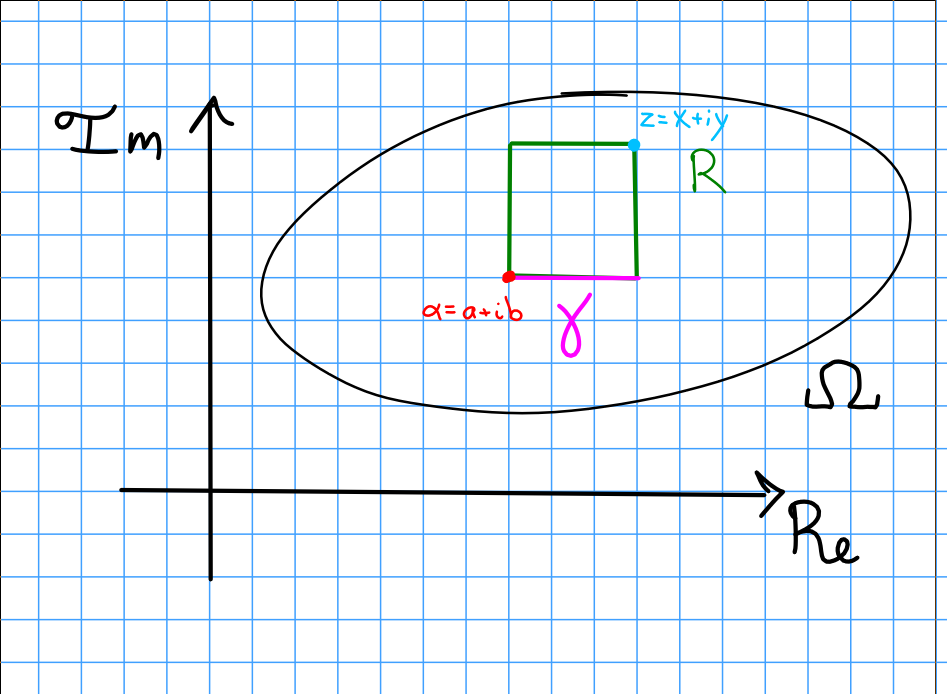
\includegraphics{figures/2020-02-03-14:15.png}\\

Then \(g(z)\) is holomorphic in \(\Omega\).
\item[Proof]
Fix a point \(\alpha = a + ib\) and given \(z = x+iy\), construct a
rectangle \(R\) containing \(z\). Then by assumption,
\(\int_{\bd R} g(z) ~dz = 0\). Let \(\gamma_{az}\) be the path given by
traversing the bottom edge of \(R\), and \(\sigma_{az}\) by the top
path.

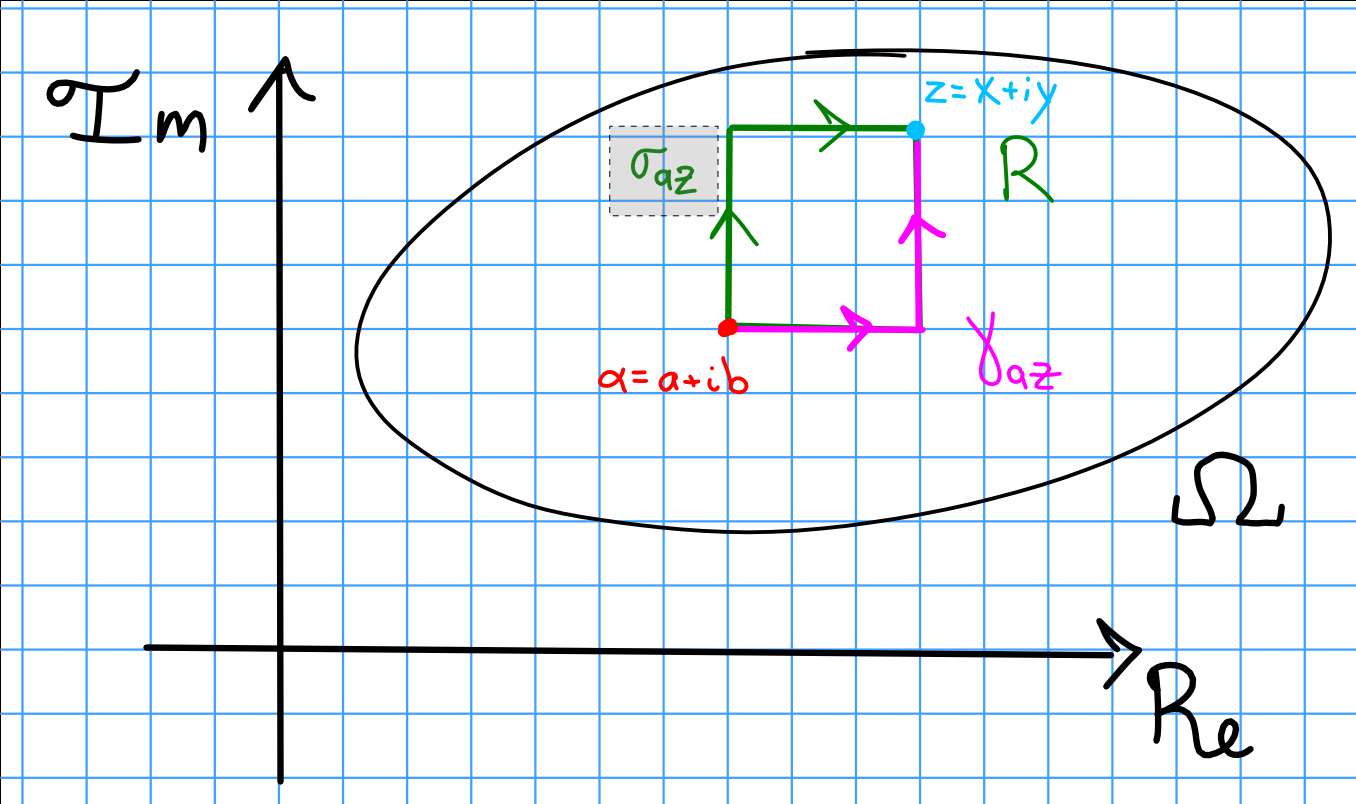
\includegraphics{figures/2020-02-03-14:24.png}\\

Let

\begin{align*}
f(z)
&= \int_{\gamma_{az} } g(z) ~dz \\
&= \int_a^x g(s+ib) ~ds + i \int_b^y g(x+it) ~dt
.\end{align*}

Since
\begin{align*}\int_{\bd R} g(z) ~dz = 0 = \int_{\gamma_{az}} \cdots - \int_{\sigma_{az}} \cdots,\end{align*}
we have

\begin{align*}
f(z) 
&= \int_{\sigma_{az}} g(z) ~dz \\
&= i \int_b^y g(a + it) ~dt + \int_x^a g(s + iy) ~ds
.\end{align*}

\begin{quote}
Exercise: Apply \(\dd{}{y}\) to the first identity and \(\dd{}{x}\) to
the second.
\end{quote}

This yields
\begin{align*}\dd{f}{x} = g(z) \quad\text{ and }\quad \dd{f}{y} = ig(z) = i \dd{f}{x}\end{align*}
by applying the FTC, which are precisely the Cauchy-Riemann equations
for \(f\). So \(f\) is holomorphic, and thus \(f(z) = g(z)\).
\end{description}

\hypertarget{wednesday-february-5th}{%
\section{Wednesday February 5th}\label{wednesday-february-5th}}

\hypertarget{cauchymorera-theorems}{%
\subsection{Cauchy/Morera Theorems}\label{cauchymorera-theorems}}

Recall last time: We have Cauchy's theorem, which says that if
\(f: \Omega \to \CC\) is holomorphic then
\begin{align*}\int_\gamma f~dz = 0.\end{align*}

We have a partial converse:

\begin{description}
\item[Theorem (Morera)]
If \(g: \Omega \to \CC\) is continuous and \(\int_R g~dz = 0\) for every
rectangle \(R\subset \Omega\) with sides parallel to the axes, then
\(g\) is holomorphic.
\item[Proof (Morera)]
Fix a point \(a\in\Omega\), then for any \(z\in\Omega\) define
\(f(z) = \int_{\gamma_{a, z}} g(\xi) d\xi = \int_{\sigma_{a, z}} g(\xi) d\xi\).

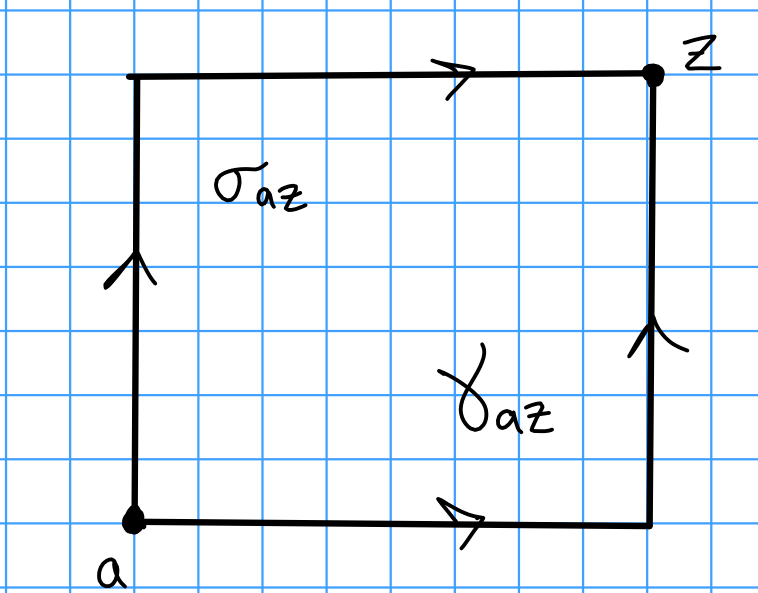
\includegraphics{figures/2020-02-05-13:42.png}\\

Then \(\dd{f}{z} = \dd{f}{x} = \frac 1 i \dd{f}{y} = g(z)\), making
\(g\) holomorphic.
\end{description}

\hypertarget{schwarz-reflection}{%
\subsection{Schwarz Reflection}\label{schwarz-reflection}}

\begin{description}
\item[Theorem (Schwarz Reflection, Extending Holomorphic Functions
Across Reflected Regions)]
Let \(\Omega = \Omega^+ \union L \union \Omega^-\) be a region of the
following form:

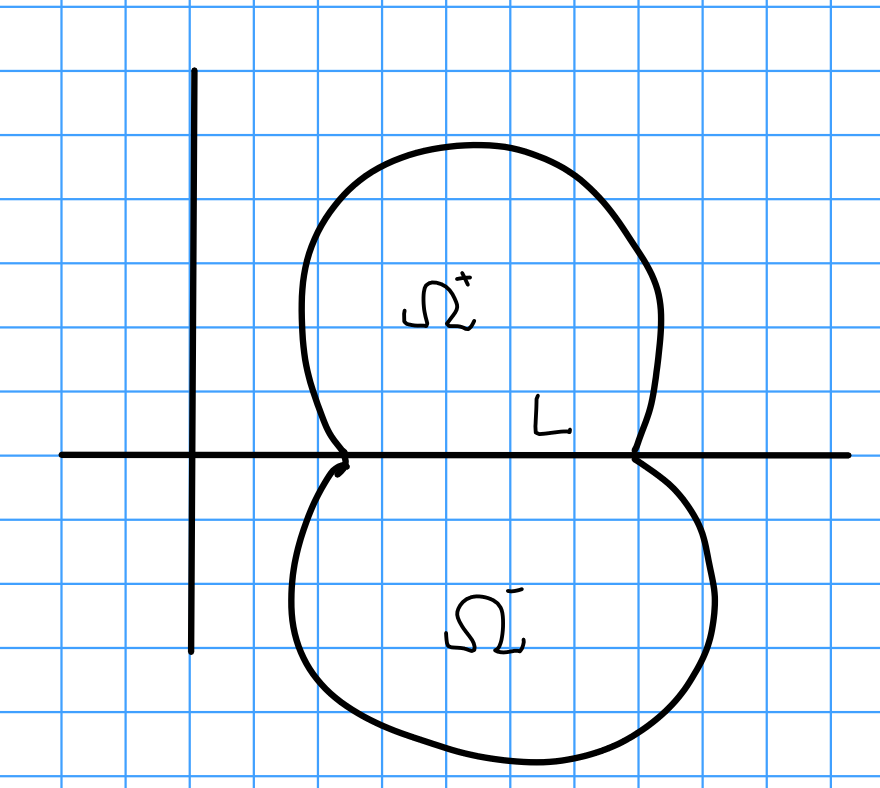
\includegraphics{figures/2020-02-05-13:45.png}\\

I.e., \(L = \theset{z\in \Omega \suchthat \im z = 0}\),
\(\Omega^{\pm} = \theset{\pm \im z > 0}\) where \(\Omega\) is symmetric
about the real axis, i.e.~\(z\in \Omega \implies \bar z \in \Omega\).

Assume that \(f: \Omega^+ \union L \to \CC\) is continuous and
holomorphic in \(\Omega^+\) and real-valued on \(L\). Define

\begin{align*}
g(z) = 
\begin{cases}
f(z) & z\in \Omega^+ \union L \\
\bar{f(z)} & z\in \Omega^-
\end{cases}
.\end{align*}

Then \(g(z)\) is defined and holomorphic on \(\Omega\).
\item[Proof (Schwarz Reflection)]
Since \(g\) is \(C^1\) in \(\Omega^-\), check that \(g\) satisfies the
Cauchy-Riemann equations on \(\Omega^-\) and thus holomorphic there. To
see that \(g\) is holomorphic on all of \(\Omega\), we'll show the
integral over every rectangle is zero.

It's clear that if \(R\subset \Omega^{\pm}\), \(\int_R g = 0\) since
\(g\) is holomorphic there, so it suffices to check rectangles
intersecting the real axis. Write \(R = R^+ \union R^-\):

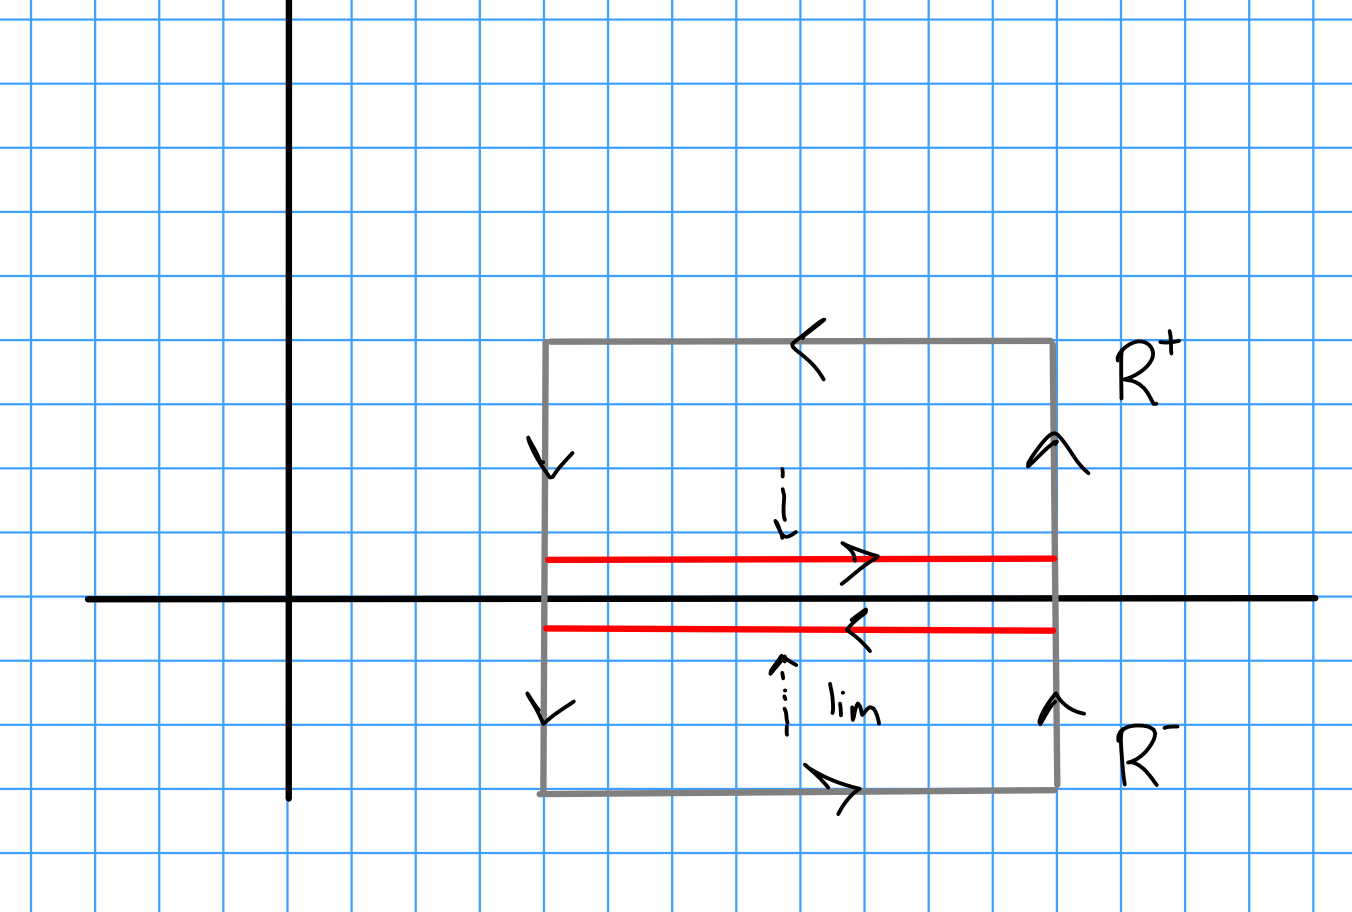
\includegraphics{figures/2020-02-05-13:59.png}\\

We then have \(R^+ = \lim_{\eps\to 0} R_\eps\) and
\(R^- = \lim_{\eps \to 0} R_{-\eps}\), and \(\int_{R_{\pm \eps}} g = 0\)
for all \(\eps > 0\). By continuity of \(f\) on \(L\), we have
\(\lim \int_{R_{\eps}} g(z) ~dz = 0\).
\end{description}

\hypertarget{goursats-theorem}{%
\subsection{Goursat's Theorem}\label{goursats-theorem}}

\begin{description}
\item[Theorem (Goursat, \(C^1\) implies smooth)]
If \(f: \Omega \to \CC\) is complex differentiable at each point of
\(\Omega\), then \(f\) is holomorphic. I.e.,
\begin{align*}f\in C^1(\Omega) \implies f\in C^\infty(\Omega).\end{align*}
\item[Proof (Goursat)]
We have \(\int_R f ~dz = 0\) for all rectangles \(R\). Write
\(I = \int_R f ~dz\). Break \(R\) into 4 sub-rectangles:

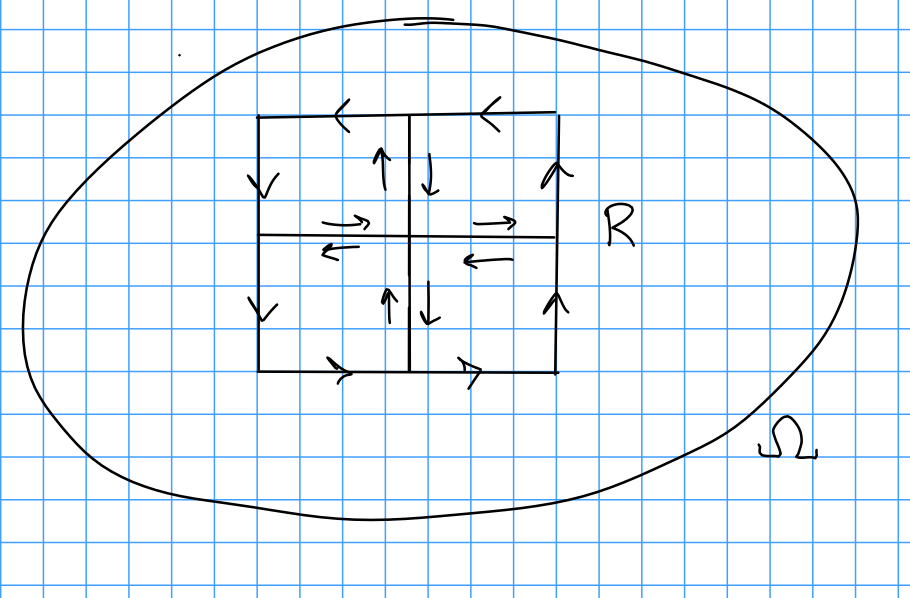
\includegraphics{figures/2020-02-05-14:08.png}\\

Then rewriting the integral and applying the triangle inequality yields

\begin{align*}
I = \int_R f = \sum_{j=1}^4 \int_{R_j} f  = \sum_{j=1}^4 I_j \implies \abs{I} \leq \sum_j \abs{I_j}
.\end{align*}

So for at least one \(j\), we have \(\abs{I_j} \geq \frac 1 4 \abs{I}\);
wlog call it \(R_1\). By continuing to subdivide, we can write

\begin{align*}
\abs I \leq 4 \abs {I_k} = 4 \abs{\int_{R_1} f} \leq 4\qty{4 \abs{ \int_{R_2} f }  } \cdots \leq 4^k \abs{\int_{R_k} f}
.\end{align*}

This is a sequence of nested compact intervals, so there is some
\(z_0 \in \intersect R_k\).

Write \(f(z) = f(z_0) + f'(z_0)(z-z_0) + \delta(z, z_0)\), and since

\begin{align*}
\lim_{z\to z_0} \frac{\abs{\delta(z, z_0)}}{z-z_0} = 0
,\end{align*}

we have \(\delta(z, z_0) = o(z-z_0)\). Then
\(\abs I \leq 4^k \frac{1}{2^k} \abs{R}\). We then try to estimate the
integral using the fact that
\(\abs{\delta(z, z_0)} \leq \delta_k \abs{z-z_0}\) for some constant
\(\delta_k \to 0\) as \(k\to \infty\).

\begin{align*}
\int_{R_k} f i
&= \int f(z_0) + f'(z_0)(z-z_0) + \delta(z, z_0) \\
&= \int_{R_k} \delta(z, z_0) \quad\text{since the first two terms are holomorphic} \\
&\leq \frac{1}{2^k} \abs{R} \delta_k \frac{C}{2^k} \abs{R} \\
& = c/4^k \abs{R}^2 \delta_k  \\
&\converges{k\to\infty}\to 0
,\end{align*}

where we use the fact that in \(R_k\) we have

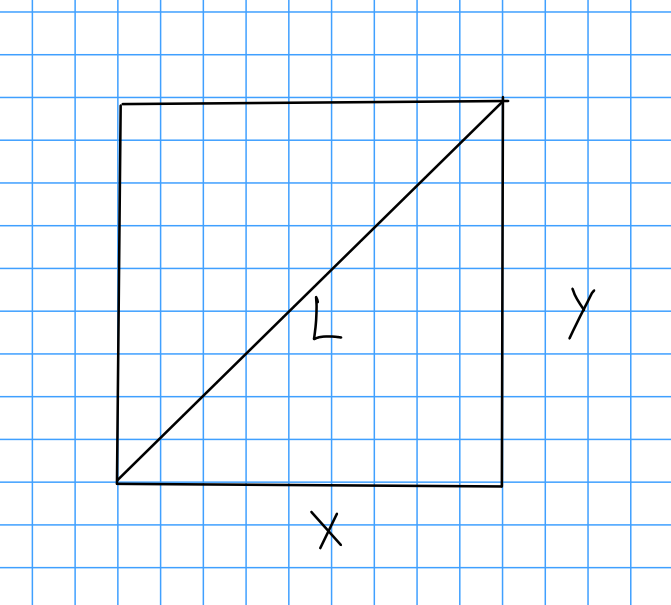
\includegraphics{figures/2020-02-05-14:23.png}\\

\begin{align*}
R_k = 2(x+y) \implies R^2/4 = x^2 + y^2 + x + y \leq_{CS} x^2 + y^2 + x^2 + y^2 = 2(x^2 + y^2) \\
\implies x^2 + y^2 \leq R^2 / 8 \implies L = \sqrt{x^2 + y^2} \leq R^8 /2\sqrt{2} \\
\implies \abs{z-z_0} \leq \sqrt{x^2+y^2} \leq R_k/2\sqrt{2} \text{ and } R_k = \frac 1 {2^k} \abs{R}
.\end{align*}

\begin{quote}
Note that triangles implies rectangles, but think about how to use
triangles to prove it for rectangles (note that sides should be parallel
to axes!)
\end{quote}
\end{description}

\hypertarget{friday-february-7th}{%
\section{Friday February 7th}\label{friday-february-7th}}

\hypertarget{sequences-of-holomorphic-functions}{%
\subsection{Sequences of Holomorphic
Functions}\label{sequences-of-holomorphic-functions}}

\begin{description}
\tightlist
\item[Theorem (The Uniform Limit of Holomorphic Functions is
Holomorphic)]
Suppose \(\theset{f_n}\to f\) is a sequence of holomorphic functions
converging uniformly on any compact subset \(K \subset \Omega\). Then
\(f\) is holomorphic.
\item[Proof]
Let \(D\) be any disc such that \(\bar D \subset \Omega\). For any
rectangle \(R \subset D\), we have
\begin{align*}\int_R f_n ~dz = 0.\end{align*} Since \(f_n \to f\)
uniformly, \(\int_R f ~dz = 0\) and thus \(f\) is holomorphic in \(D\).
\end{description}

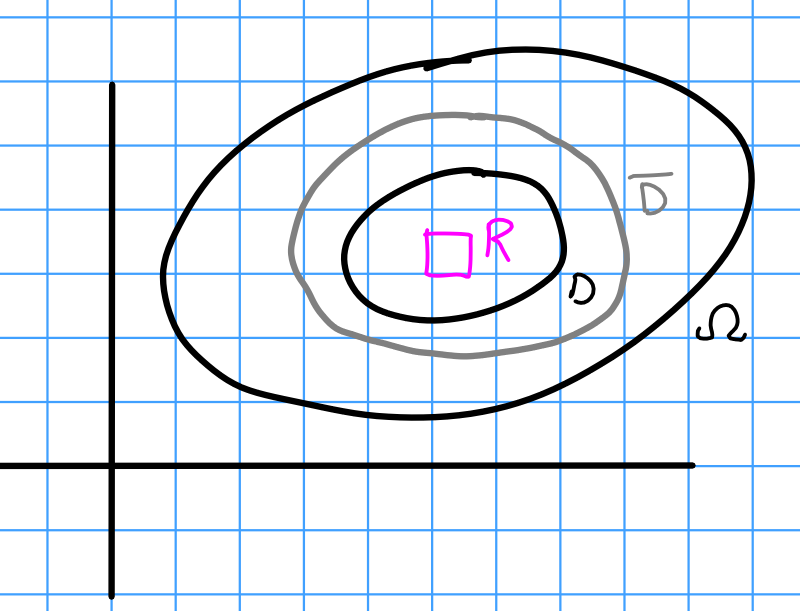
\includegraphics{figures/2020-02-07-13:36.png}\\

\begin{description}
\item[Theorem (Uniform Convergence of Derivatives)]
Under the same hypotheses, \(f_n' \to f\) uniformly on any compact
subset \(K \subset \Omega\).
\item[Proof]
See Stein.
\item[Corollary (When Functions Defined by Integrals are Holomorphic)]
Suppose \(F(z, s): \Omega \cross [a, b] \to \CC\) and

\begin{enumerate}
\def\labelenumi{\arabic{enumi}.}
\item
  \(F(z, s)\) is holomorphic in \(z\) for each fixed \(s \in [a, b]\).
\item
  \(F(z, s)\) is continuous in \(\Omega \cross [a, b]\).
\end{enumerate}

Then \(f(z) = \int_a^b F(z, s) ~ds\) is holomorphic on \(\Omega\).
\item[Proof]
Define \(f_n(z) = \qty{ \sum_{k=1}^n F(z, s_k) } \frac{b-a}{n}\) where
each \(s_k = a + \frac{b-a}{n} k \in [a, b]\). Need to show \(f_n(z)\)
converges uniformly on any compact \(K \subset \Omega\), i.e.~it's
uniformly Cauchy. Fix \(K\) compact, then by a theorem in topology
\(K \cross [a,b]\) is again compact.

Using the fact that \(F\) is continuous on a compact set and thus
uniformly continuous, fix \(\eps > 0\) and find \(\delta>0\) such that
\(\max_{z\in K} \abs{F(z, s) - F(z, t)} < \eps\) for all
\(s,t \in [a, b]\) with \(\abs{t-s} < \delta\).

Thus if \(\frac{b-a}{n} < \delta\) and \(z\in K\), we have an estimate

\begin{align*}
\abs{f_n(z) - f(z)} 
&= \abs{ \sum_{k=1}^n \int_{s_{k-1}}^{s_k} F(z, s_k) - F(z, s) ~ds } \\
&= \sum_{k=1}^n \int_{s_{k-1}}^{s_k} \abs{ F(z, s_k) - F(z, s) } ~ds \\
&\leq \eps \qty{b-a} 
.\end{align*}

Thus \(f_n \converges{u}\to f\).
\end{description}

Remark: this is useful for showing
\begin{align*}\Gamma(z) = \int_0^\infty e^{-s} s^{z-1} ~ds\end{align*}
is holomorphic for \(\Re z > 0\).

\hypertarget{uniform-approximation}{%
\subsection{Uniform Approximation}\label{uniform-approximation}}

\textbf{Question}: can every function be uniformly approximated by
polynomials?

\textbf{Answer}: in general, no. Take \(f(z) = \frac 1 z\), which is
holomorphic on \(\CC \setminus 0\), but \(\int_\gamma P_N(z) = 0\) for
any polynomial (since )hey are entire) for any loop \(\gamma\) around 0,
but \(\int_\gamma \frac 1 z = 2\pi i\).

\begin{description}
\item[Theorem (Uniform Approximation by Polynomials (Stein 5.2))]
If \(f_n\) is a sequence of holomorphic functions converging uniformly
on any compact subset \(K\) of \(\Omega\) then \(f\) is holomorphic in
\(\Omega\) and if \(f(z) = \sum a_n (z- z_0)^n\) then
\(P_N(z) = \sum^N a_n (z-z_0)^n\).
\item[Theorem (Uniform Approximation by Rational Functions (Stein 5.7))]
Any holomorphic function in a neighborhood of a compact set \(K\) can be
approximated by a \emph{rational} function with singularities only in
\(K^c\). If \(K^c\) is connected, it can be approximated by a
\emph{polynomial}.
\item[Lemma (5.8, ???)]
Suppose \(f\) is holomorphic in an open set \(\Omega\) with
\(K\subset \Omega\) compact. Then there exist finitely many segments
\(\theset{\gamma_i}_{i=1}^N\) in \(\Omega\setminus K\) such that for all
\(z\in K\), ???.
\item[Proof (of Lemma, Idea)]
Divide region into squares, take \(\gamma_i\) to be line segments such
that they enclose \(K\). \begin{align*}
f(z) 
&= \frac{1}{2\pi i} \sum_{n=1}^N \int_{\omega_n} \frac{f(\xi)}{z-\xi} ~d\xi \\
&= \frac{1}{2\pi i} \int_{\Gamma} \frac{f(\xi)}{z-\xi} ~d\xi
.\end{align*}

where we can rewrite
\begin{align*}
\int_{\gamma_n} \cdots = \int_0^1 \frac{f(\gamma_n(t))}{\gamma_n(t) - z_0} \gamma_n'(t) ~dt = \int_0^1 F(z, s) ~ds
\end{align*}

The idea is that we can then write
\(\frac 1 {\xi - z} = \frac 1 \xi \frac 1 {1-\frac{z}{\xi}} = \xi\inv \sum_k \qty{\frac{z}{\xi}}^k\),
which allows uniform approximation by polynomials.
\end{description}

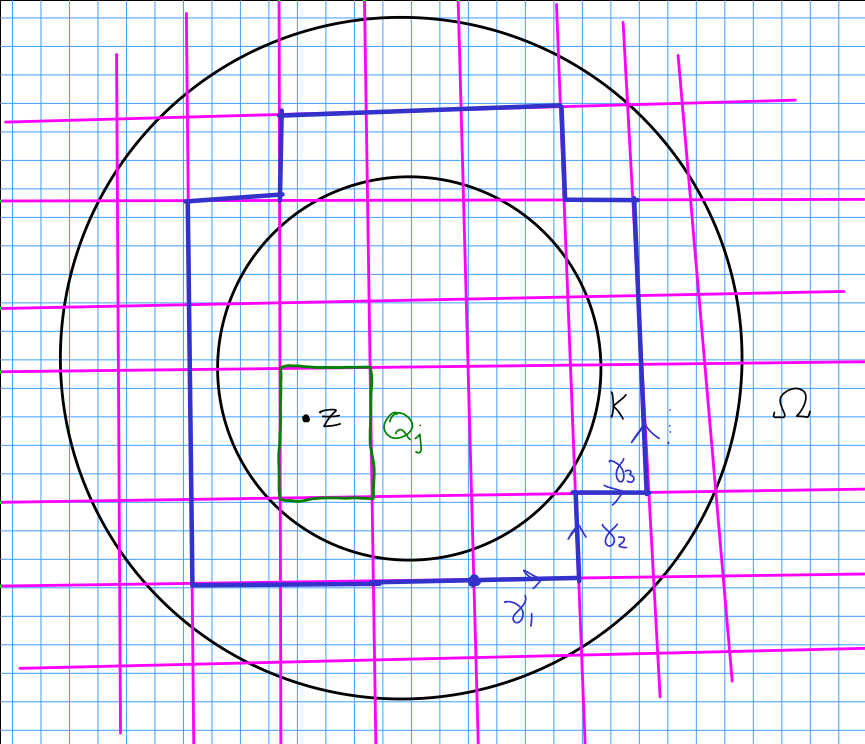
\includegraphics{figures/2020-02-07-19:51.png}\\

\hypertarget{wednesday-february-12th}{%
\section{Wednesday February 12th}\label{wednesday-february-12th}}

\hypertarget{singularities}{%
\subsection{Singularities}\label{singularities}}

Let \(f(z)\) be holomorphic on \(\Omega\), then we have Cauchy's
integral formula:

\begin{align*}
f(z) = \frac{1}{2\pi i} \int_\gamma \frac{f(\xi)}{\xi - z} ~d\xi
.\end{align*}

\emph{Example:} Note that \(f(z) = \frac 1 z\) is holomorphic on
\(\CC\setminus 0\).

Let \(\Omega\) be an open set containing a disk \(D\) and
\(\Omega\setminus p\) be a punctured domain.

\begin{description}
\item[Definition (Isolated Singularities)]
We say \(f\) has an \emph{isolated singularity} at \(p\) iff \(f\) is
defined and holomorphic on some deleted neighborhood of \(p\).

Classification of singularities:

\begin{enumerate}
\def\labelenumi{\arabic{enumi}.}
\item
  \textbf{Removable}: \(\abs{f(z)}\) is bounded on some
  \(D_r(p) \setminus p\).

  \emph{Example}: \(f(z) = \sin(z)/z\).
\item
  \textbf{Poles}: \(\lim_{z\to p} \abs{f(z)} = \infty\).

  \emph{Example}: \(f_n(z) = \frac{1}{z^n}\) at \(p=0\)
\item
  \textbf{Essential}: neither 1 nor 2.

  \emph{Example}: \(f(z) = e^{\frac 1 z}\) at \(z=0\).
\end{enumerate}
\end{description}

Note that for singularities at \(\infty\), we can just make the change
of variables \(z\mapsto \frac 1 z\). Defining \(F(z) = f(\frac 1 z)\),
the singularities at 0 of \(f\) correspond to singularities at infinity
for \(F\).

\hypertarget{spherical-projection}{%
\subsection{Spherical Projection}\label{spherical-projection}}

We can solve for a spherical projection map \(S^2 \to \CC\). Let
\((0,0,1)\) be the North pole of the sphere; then to map to
\((x, y, 0)\) on the plane we can take the parameterization
\(\ell: (tx, ty, 1-t)\). This yields

\begin{align*}
t \mapsto \qty{ \frac{2\Re(z)}{1 + \abs z^2} , \frac{2\Im(z)}{1 + \abs z^2}, 1 - \frac{2}{1 + \abs z^2}}
.\end{align*}

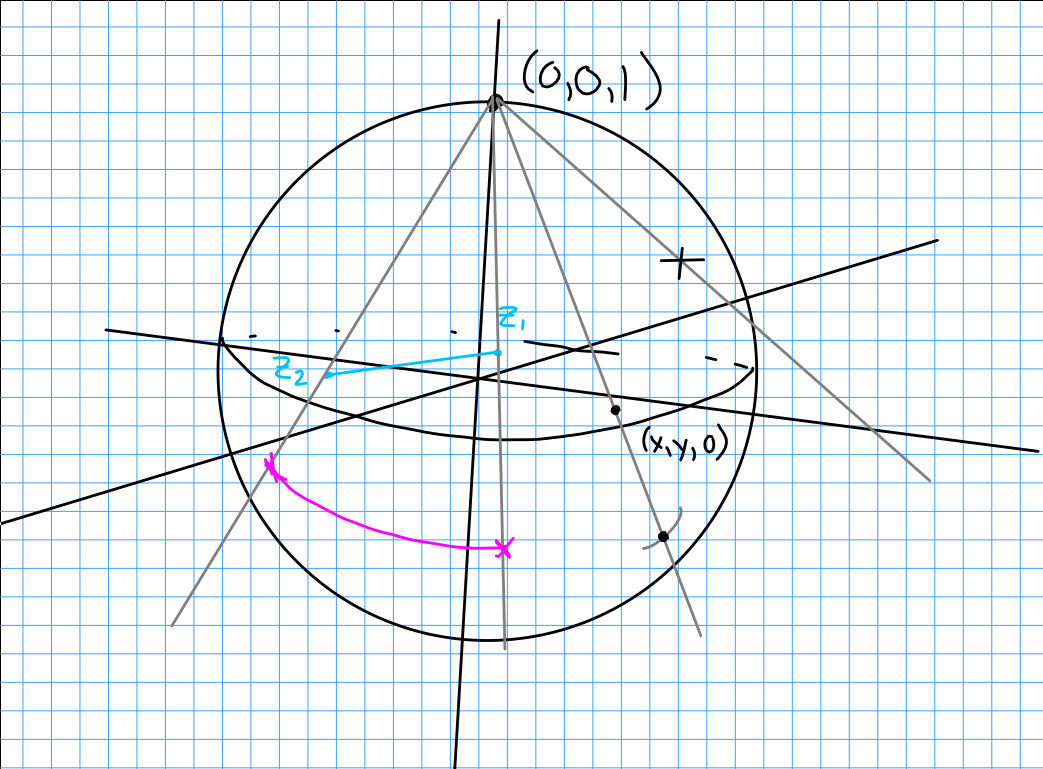
\includegraphics{figures/2020-02-12-14:05.png}\\

From this we can induce a spherical metric:

\begin{align*}
\phi(z_1, z_2) &= \frac{z \abs{z_1 - z_2}} { \sqrt{\abs z_1^2 + 1} \sqrt{\abs z_2^2 + 1}  }
.\end{align*}

\begin{description}
\item[Proposition (Continuous Extension Over Removable Singularities)]
Let \(p\) be a removable singularity of \(f\). Then

\begin{enumerate}
\def\labelenumi{\arabic{enumi}.}
\item
  \(\lim_{z\to p} f(z)\) exists.
\item
  The function \begin{align*}
  \tilde f(x) = \begin{cases}f(z) & z\neq p \\ \lim_{z\to p} f(z) & z=p  \end{cases}
  .\end{align*} is holomorphic on \(D_r(p)\).
\end{enumerate}
\item[Example]
Consider
\begin{align*}\frac{\sin(z)}{z} \converges{z\to 0}\to 1.\end{align*}
\item[Proof (of Proposition)]
Take \(p=0\) and consider \(g(z) = z^2 f(z)\). We can verify directly
that \(g\) satisfies the Cauchy-Riemann equations on \(D_r(0)\). Then
\(g\) is holomorphic on \(D_r(0)\) and vanishes to order 2 at \(z=0\),
and
\begin{align*}f(z) = \frac{g(z)}{z^2}\end{align*} is holomorphic on
\(D_r(0)\).

If \(f(z)\) has a pole at \(z_0\), then
\(\lim_{z\to z_0} \abs{f(z)} \to \infty\) by definition, iff
\(\lim_{z\to z_0} \frac{1}{\abs{f(z)}} = 0\) and thus the reciprocal has
a zero at \(z=z+0\). If \(z_0\) is a zero of a nontrivial holomorphic
function \(f\), then \(z_0\) is isolated, i.e.~there exists a punctured
disc \(D_r(z_0)\setminus z_0\) on which \(f\) is nonzero.
\item[Theorem (???)]
If \(f\) is holomorphic in a connected domain \(\Omega\) with a zero
\(z_0\), then there exists a non-vanishing holomorphic function \(g(z)\)
and some \(n\in \NN\) such that
\begin{align*}f(z) = (z-z_0)^n g(z)\end{align*}.
\item[Proof]
Since \(f\) is holomorphic, expand its power series
\(f(z) = \sum a_k (z-z_0)^k\). Since \(f(z_0) = 0\), we have
\(a_0 = 0\). Choose the smallest \(n\) such that \(a_n \neq 0\), so
\begin{align*}
f(z) 
&= a_n(z-z_0)^n + a_{n+1}(z-z_0)^{n+1} + \cdots \\
&= (z-z_0)^n \qty{a_n + \cdots} \\
&\definedas (z-z_0)^n g(z)
.\end{align*}

Then \(g(z_0) \neq 0\), so by continuity there exists an \(r\) such that
\(\abs{g(z)} \geq \abs{a_n}/2\).
\item[Definition (Pole)]
A function \(f\) defined on a deleted neighborhood of \(z_0\) has a
\textbf{pole} at \(z_0\) if the function \(F = \frac 1 f\) with
\(F(z_0) \definedas 0\) is holomorphic in a full neighborhood of
\(z_0\).
\end{description}

\hypertarget{friday-february-14th}{%
\section{Friday February 14th}\label{friday-february-14th}}

\hypertarget{defining-residues}{%
\subsection{Defining Residues}\label{defining-residues}}

\begin{quote}
Interesting open problems: dynamical systems on \(\CC^2\).
\end{quote}

If \(f\) is holomorphic in \(\Omega\) with \(f(z_0) = 0\) then there
exists a disc on which \(f(z) = \sum a_n (z-z_0)^n\) where
\(a_0 = f(z_0) = 0\). There is then a minimal \(k\) such that
\(f(z) = (z-z_0)^k g(z)\) where \(g(z_0)\neq 0\); this \(k\) is the
\emph{order} of the zero \(a_0\).

Recall the definition of a \emph{pole}: A function defined in a deleted
neighborhood of \(z_0\) has a \emph{pole} at \(z_0\) iff
\(F = \frac 1 f\) with \(F(z_0) \definedas 0\) is holomorphic in a full
neighborhood of \(z_0\).

\begin{description}
\item[Theorem (Extraction of Holomorphic Part)]
If \(f\) has a pole at \(z_0\), then there exists a holomorphic function
\(h\) and a unique \(k\) such that \(f(z) = (z-z_0)^{-k} h(z)\).
\item[Proof]
Write
\begin{align*}\frac 1 f = (z-z_0)^k g(z)\end{align*} with
\(g(z_0) \neq 0\). Then there is an \(r\) such that
\(\abs{g(z)} \geq \frac 1 2 \abs{g(z_0)}\) in a disc about \(z_0\). Then
\begin{align*}f(z) = \frac{1}{\qty{z-z_0} g(z)} \definedas (z-z_0)^{-k} h(z)\end{align*}
where \(h = 1/g\).

We can then write
\begin{align*}f(z) = \qty{ \sum_{i=0}^{k-1} b_k (z-z_0)^{-k} } + b_k + \sum_{i=1}^\infty b_{k+i} (z-z_0)^i\end{align*}
for some fixed \(k\), where \(\sum b_i (z-z_0)^i\) is the power series
expansion of \(h\). Write this as \(P(z) + G(z)\) where
\(G(z) = \sum_{i=0}^\infty b_{i+k}(z-z_0)^i\). Denote \(P\) \emph{the
principal part} of \(f\) at the pole \(z=z_0\).

Note that
\begin{align*}\int_{D_r(z_0)} f = \int_{D_r(z_0)} P(z) = 2\pi i ~a_{-1}.\end{align*}
\item[Definition (Residue)]
The coefficient \(a_{-1}\) is referred to as the \emph{residue} of \(f\)
at \(z=z_0\).
\end{description}

\hypertarget{residues}{%
\subsection{Residues}\label{residues}}

Note that
\begin{align*}\int \frac{1}{\qty{z-z_0}^k} = \begin{cases} 2\pi i &k = 1 \\ 0 & \text{else}\end{cases}.\end{align*}

Residues can be computed using the following formula: \begin{equation}
a_{-1} = \frac 1 {2\pi i} \int_{D_r(z_0)} f
.\end{equation}

Theorem (Residue Formula) : \begin{align*}
    \Res_{z=z_0} f = \lim_{z\to z_0} \frac{1}{\qty{k-1}!} \qty{\dd{}{z}}^{k-1} (z-z_0)^k f(z)
    .\end{align*}

\begin{description}
\tightlist
\item[Proof]
Expand in power series, direct check.
\end{description}

A useful special case: if \(z_0\) is a pole of order 1, then

\begin{align*}
\Res_{z=z_0} f = \lim_{z\to z_0} (z-z_0) f(z)
.\end{align*}

A useful formula:

\begin{align*}
\frac 1 {2\pi i} \int_{\Gamma(z_0)} f = \Res_{z=z_0} f
.\end{align*}

\begin{description}
\item[Theorem (Integral Residue Theorem)]
Suppose that \(f\) is holomorphic in an open set containing a toy
contour \(\gamma\) and its interior except for finitely many poles
\(\theset{z_i}\). Then

\begin{align*}
\frac 1 {2\pi i} \int_\gamma f = \sum \Res_{z=z_i} f(z)
.\end{align*}
\item[Proof]
Omitted to cover some material needed for homework.
\end{description}

Note that if \(f\) has a pole of order \(k\), we can expand it in
\emph{Laurent series} as

\begin{align*}
\sum_{n=-k}^1 a_n (z - z_0)^n + \sum_{n=0}^\infty a_n(z-z_0)^k
.\end{align*}

How to determine the radius of convergence\index{Radius of convergence}
of a Laurent series:

\begin{align*}
\sum_{-\infty}^\infty a_n z_n
&= \sum_{n\in \NN} c_n z^n + \sum_{n\in \NN} d_n z^{-n} 
.\end{align*}

Applying the root test,

\begin{align*}
\limsup_n \abs{c_n (z-a)}^{1/n} &< 1 \\
\iff \limsup_n \abs{c_n}^{1/n} \abs{z-z_0}^n &< 1 \\
\iff \abs{z-a} &\leq \frac{1}{\limsup_n \abs{c_n}^{1/n}} \definedas \rho_1
.\end{align*}

Similarly, we need

\begin{align*}
\rho_2 \definedas \limsup_n \abs{d_n}^{1/n} < \abs {z-a}
.\end{align*}

If \(\rho_1> \rho_2\), this will converge on an annulus.

\hypertarget{monday-february-17th}{%
\section{Monday February 17th}\label{monday-february-17th}}

\begin{quote}
See Hans Lewy 1957 Annals, Folland and Stein 1973. Does a linear system
of PDEs with analytic functions have an analytic solution? What about
just \(C^\infty\)?
\end{quote}

\hypertarget{getting-a-holomorphic-function-from-a-laurent-series}{%
\subsection{Getting a Holomorphic Function from a Laurent
Series}\label{getting-a-holomorphic-function-from-a-laurent-series}}

We can write a formal series \begin{align*}
f(z) &= \sum_{n\in \ZZ}a_n (z-a)^n \\
&= \sum_{n\geq 0} a_n (z-z_0)^n + \sum{n\leq -1} a_n (z-z_0)^n \\
&\definedas A(z) + B(z)
.\end{align*}

Part \(A\) converges for
\begin{align*}\abs{z-a} < R_1 = \qty{\limsup \abs{x_n}^{1/n}} \inv.\end{align*}
Part \(B\) converges for
\begin{align*}\abs{z-a} > R_2 = \limsup \abs{c_{-n}}^{1/n}.\end{align*}

If \(R_1 < R_2\), this does not converge. Note that if \(R_1 > R_2\),
then \(f\) converges and defines a holomorphic function on the annulus
\(R_2 < \abs{z-a} < R_1\). Moreover, \(f\) converges uniformly on any
compact subset of this annulus, so it can be differentiated
term-by-term, and the derivative has the same region of convergence.

Note that if \(f\) equals its Laurent expansion, then
\begin{align*}c_n = \frac{f^{(n)}(a)}{n!} = \frac 1 {2\pi i} \int_\gamma \frac{f(\xi)}{\qty{\xi - a}^{n+1}} ~dz\end{align*}
where \(\gamma\) is contained in the annulus of convergence, and
\(c_{n\leq -1} 0\).

We also have

\begin{align*}
\frac 1 {2\pi i} \int_\gamma \frac{f(z)}{(z-a)^m} ~dz 
&= \sum_{n\in \ZZ} \frac{c_n}{2\pi i} \int_\gamma \frac{1}{(z-a)^{m-n}}~dz \\
&=c_{m-1}
,\end{align*}

since
\begin{align*}\int_\gamma \frac{1}{\qty{z-a}^k}~dz = \begin{cases} 2\pi i &k = 1 \\ 0 & \text{else}\end{cases},\end{align*}
we have the following formula for the coefficients:

\begin{align}
c_m &= \frac 1 {2\pi i} \int_\gamma \frac{f(z)}{\qty{z-a}^{m+1}} ~dz
.\end{align}

So we can start with a series and get a holomorphic function on some
region.

\hypertarget{obtaining-a-laurent-series-from-a-holomorphic-function}{%
\subsection{Obtaining a Laurent Series from a Holomorphic
Function}\label{obtaining-a-laurent-series-from-a-holomorphic-function}}

We can also start with a holomorphic function and get a Laurent series.
Suppose \(f\) is holomorphic on an annulus \(R_2 < \abs {z} < R_1\). We
can then write

\begin{align*}
f(z) = \frac 1 {2\pi i} \int_{\abs{w-a} = R_1} \frac{f(w)}{w-z} ~dw - \int_{\abs{w-z} = R_2} \frac{f(w)}{w-z} ~dw
\end{align*}

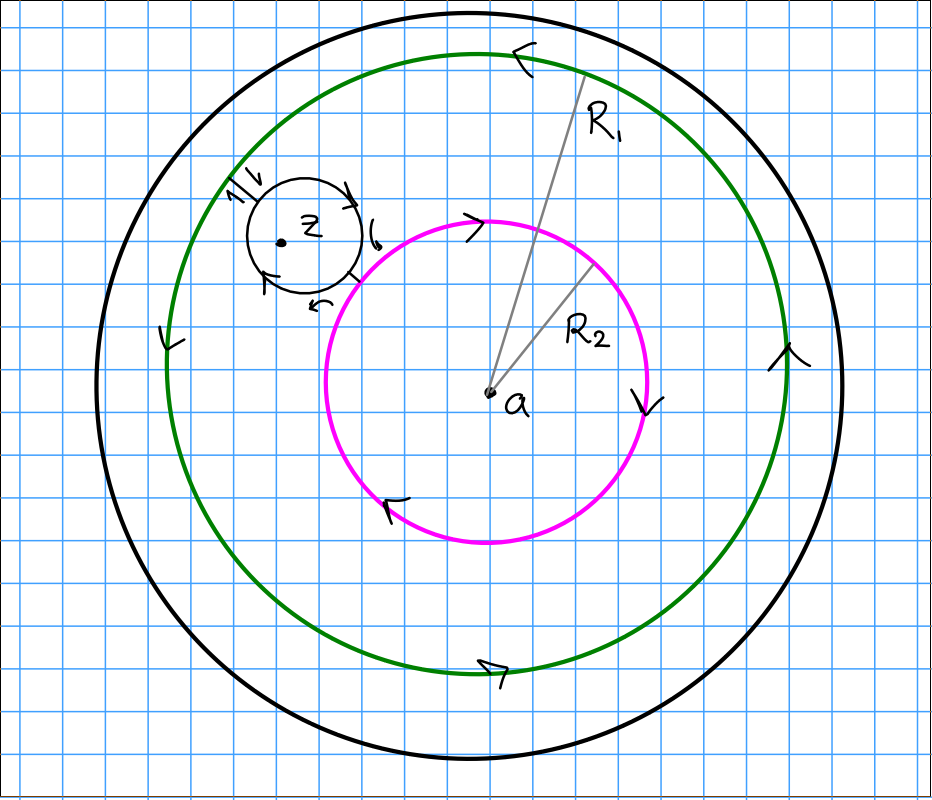
\includegraphics{figures/2020-02-17-14:07.png}\\

Since \(\abs{z-a}/\abs{w-a} < 1\), we have

\begin{align*}
\frac {1}{2\pi i} \int_{\abs{w-a} = R_1} \frac{f(w)}{w-z} ~dz 
&= \frac {1}{2\pi i} \int_{\abs{w-a} = R_1} \frac{f(w)}{(w-a) - (z-a)} ~dz \\
&= \frac {1}{2\pi i} \int_{\abs{w-a} = R_1} \frac{f(w)}{(w-a)} \sum_{n\in \NN} \frac{(z-a)^n}{(w-a)^n} ~dz \\
&= \sum_{n\in \NN} (z-a)^n \frac 1 {2\pi i} \int_{\abs{w-a} = R_1} \frac{f(w)}{(w-a)^{n+1}} ~dw \\
&= \sum_{n\in \NN} c_n (z-a)^n
.\end{align*}

Similarly,

\begin{align*}
-\frac 1 {2\pi i} \int_{\abs{w-a} = R_2}  \frac{f(w)}{w-z} ~dw  
&= -\frac 1 {2\pi i} \int_{\abs{w-a} = R_2} \frac{f(w)}{(w-a) - (z-a)} ~dw  \\ 
&= -\frac 1 {2\pi i} \frac {1}{z-a} \int_{\abs{w-a} = R_2} \frac {f(w)} {\frac{w-a}{z-a} - 1} ~dw  \\
&= \frac 1 {2\pi i} \frac {1}{z-a} \int_{\abs{w-a} = R_2}  \frac{f(w)} {1 - \frac{w-a}{z-a} } ~dw  \\
&= \frac 1 {2\pi i} \frac {1}{z-a} \int_{\abs{w-a} = R_2} f(w) \sum_{n\in \NN} \frac{(w-a)^n}{(z-a)^n} ~dw \\
&= \sum_{n\in\NN} \frac 1 {2\pi i} \frac {1}{(z-a)^{n+1}} \int_{\abs{w-a} = R_2} f(w) (w-a)^n ~dw  \\ 
&= \sum_{n=-\infty}^{-1} c_n (z-a)^n
.\end{align*}

This yields a formula

\begin{equation}
c_m = \frac {1}{2\pi i} \int_\gamma \frac{f(z)}{(z-a)^{m+1}} ~dz
.\end{equation}

In practice, we don't use this formula for extracting coefficients.

\begin{description}
\item[Example]
Let \(f(z) = \frac{1}{z(z-1)}\). This has four Laurent series.

Let \(C(a, R_1, R_2)\) be the annulus centered at \(a\). Then at
\(C(0, 0, 1) = \DD\setminus \theset{0}\), we have

\begin{align*}
f(z) = \frac 1 z \frac 1 {1-z} = -\frac 1 z \sum_{k\in \NN} z^k
.\end{align*}

In \(C(1, 1, 0) = \DD(1, 1) \setminus\theset{1}\), we have

\begin{align*}
f(z) 
&= \frac 1 {z-1} \frac 1 z \\
&= \frac 1 {z-1} \frac 1 {1 + (z-1)} \\
&= \frac 1 {z-1} \sum_{k\in \NN} (-1)^k (z-1)^k
.\end{align*}

In \(C(0, 1, \infty)\), we can write

\begin{align*}
f(z) 
&= \frac 1 {z^2} \frac 1 {1 - \frac 1 z} \\
&= \frac 1 {z^2} \sum_{k\in \NN} \frac 1 {z^k}
.\end{align*}

And in \(C(1,1,\infty)\) we have

\begin{align*}
f(z) &= \frac 1 {z-1} \frac{1}{z-1+1}
.\end{align*}
\end{description}

\hypertarget{friday-february-21st}{%
\section{Friday February 21st}\label{friday-february-21st}}

\hypertarget{singularities-1}{%
\subsection{Singularities}\label{singularities-1}}

Recall that there are three types of singularities:

\begin{itemize}
\tightlist
\item
  Removable
\item
  Poles
\item
  Essential
\end{itemize}

Recall that a function \(g\) is holomorphic at \(z_0\) iff
\begin{align*}
\lim_{z\to z_0}  (z-z_0) g(z) = 0
\end{align*}

\begin{description}
\item[Theorem (3.2)]
An isolated singularity \(z_0\) of \(f\) is a pole
\(\iff \lim_{z\to z_0} f(z) = \infty\).
\item[Theorem (3.3, Casorati-Weierstrass)]
If \(f\) is holomorphic in \(D_r(z_0) \setminus \theset{z_0}\) and has
an essential singularity \(z_0\), then there exists a radius \(r\) such
that \(f(D_r(\theset{z_0})\setminus \theset{z_0})\) is dense in \(\CC\).
\item[Proof]
Proceed by contradiction. Suppose there exists a \(w\in \CC\) and a
\(\delta > 0\) such that
\begin{align*}
D_\delta(w) \intersect f(D_r(\theset{z_0})\setminus \theset{z_0}) = \emptyset
.\end{align*}

If \(z \in D_r(w)\setminus{z_0}\), then \(\abs{f(z) - w} > \delta\).
Define \(g(z) = \frac{1}{f(z) - w}\) on
\(D_r(z_0) \setminus\theset{z_0}\); then
\(\abs{g(z)} < \frac{1}{\delta}\).

\begin{quote}
Note that this implies that \(g(z)\) is holomorphic on
\(D_r(z_0) \setminus \theset{z_0}\). \(g(z)\) being holomorphic here
follows from \(f\) being holomorphic here.
\end{quote}

Then \(g(z)\) has a removable singularity at \(z = z_0\) by theorem 3.1.

If \(g(z_0) \neq 0\), then \(f(z) - w\) is holmorphic at \(z_0\),
contradicting the fact that \(z_0\) is an essential singularity.

If instead \(g(z_0) = 0\), then \(z_0\) is a pole, again a
contradiction.
\end{description}

\begin{quote}
Note: revisit why this is a contradiction.
\end{quote}

\hypertarget{singularities-at-infinity}{%
\subsection{Singularities at Infinity}\label{singularities-at-infinity}}

The point \(z=\infty\) can be one of three types of singularities:

\begin{enumerate}
\def\labelenumi{\arabic{enumi}.}
\item
  \emph{Removable} \(\iff\)
  \(f(z) = \sum_{k=-1}^\infty c_k \frac{1}{z^k}\).

  \begin{itemize}
  \tightlist
  \item
    I.e. only one positive exponent.
  \end{itemize}
\item
  \emph{Pole} \(\iff\) \(f(z) = \sum_{k = -\infty}^n c_k z^k\)

  \begin{itemize}
  \tightlist
  \item
    I.e. there are finitely many positive exponents.
  \end{itemize}
\item
  \emph{Essential} \(\iff\) \(f(z) = \sum_{k=-\infty}^\infty c_k z^k\)

  \begin{itemize}
  \tightlist
  \item
    There are infinitely many positive exponents.
  \end{itemize}
\end{enumerate}

\begin{description}
\item[Definition (Meromorphic)]
A function \(f\) is \textbf{meromorphic} on \(\Omega\) iff there exists
a sequence \(\theset{z_i} \subset \Omega\) with no limit point in
\(\Omega\) such that

\begin{enumerate}
\def\labelenumi{\arabic{enumi}.}
\tightlist
\item
  \(f\) is holomorphic on \(\Omega \setminus\theset{z_i}\), and
\item
  \(f\) has poles at each \(z_i\).
\end{enumerate}
\item[Theorem (3.4, Meromorphic Functions are Rational)]
\(f\) is meromorphic on \(\CP^1\) iff \(f\) is a rational function.
\item[Proof]
\hfill

\(\implies\): By part 1 of the definition above, the point \(z=0\) is
either a pole or a removable singularity of the function
\(F(z) = f\qty{\frac 1 z}\). By part 2, \(F\) has finitely many poles
\(\theset{z_k}_{k=1}^N\). So for each \(k\), write
\begin{align*}
f(z) = f_k(z) + g_k(z)
\end{align*} where \(f_k\) is the principal part and \(g_k\) is
holomorphic in a neighborhood of \(z_k\). Then \(f_k(z)\) is a
polynomial in \(\qty{\frac 1 {z-z_k}}\), say of degree \(m_k\). But then
\begin{align*}
F(z) \definedas f\qty{\frac 1 z} = \tilde f_\infty(z) + \tilde g_\infty(z)
\end{align*} where \(\tilde f_\infty(z)\) is a polynomial in \(z\), and
\(\tilde g_\infty(z)\) is holomorphic near zero. Thus
\(\tilde f_\infty\qty{\frac 1 z}\) is a polynomial in \(\frac 1 z\).

Define \(f_\infty(z) = \tilde f_\infty \qty{\frac 1 z}\) and
\begin{align*}
H(z) = f(z) - f_\infty (z) - \sum_k f_k(z)
.\end{align*}

Then \(H\) is entire and bounded and thus constant, and since
\(\lim_{z\to \infty} H(z) = 0\), \(H\) is identically zero. Thus
\begin{align*}
f(z) = f_\infty(z) + \sum_k f_k(z)
\end{align*}

\hfill\break

\(\impliedby\): To be continued, uses the argument principle, Rouche's
theorem, and Jordan's lemma.
\end{description}

\hypertarget{wednesday-february-26th}{%
\section{Wednesday February 26th}\label{wednesday-february-26th}}

\hypertarget{argument-principle-and-application}{%
\subsection{Argument Principle and
Application}\label{argument-principle-and-application}}

Let \(f\) be holomorphic in \(\Omega\) which is open, simple, and
connected. Then \(f(z_0) = 0\) implies there exists an integer \(m\)
such that \(f(z) = (z-z_0)^m g(z)\) where \(g(z_0) \neq 0\).

Let \(N_\Omega(f)\) be the number of zeros of \(f\) inside \(\Omega\),
and \(N_\Omega(f, a)\) be the number of zeros of \(f-a\) in \(\Omega\).
Writing \(f = f_1 f_2\) where \(f_1 = (z-z_0)^m\) and \(f_2 = g(z)\), we
have

\begin{align*}
\frac {f'} f
&= \frac {f_1'} {f_1} + \frac {f_2'} {f_2} \\
&= \frac m {z-z_0} + \frac {g'} g
.\end{align*}

Now integrating both sides yields

\begin{align*}
\frac 1 {2\pi i } \int_{D_r(z_0)} \frac{f'(z)}{f(z)} ~dz = m
,\end{align*}

so the integral of this function counts the number of zeros of \(f\) in
\(D_r(z_0)\).

\begin{description}
\tightlist
\item[Proposition (Argument Principle)]
Let \(f\) be holomorphic in a neighborhood of \(\bar{D_r(z_0)}\) and
suppose that \(f\) is non-vanishing on all of \(\bd D_r(z_0)\). Then
\end{description}

\begin{align*}
  \frac 1 {2\pi i } \int_{D_r(z_0)} \frac{f'(z)}{f(z)} ~dz = N_{D_r(z_0)}(f)
  .\end{align*}

More generally, if \(q(z)\) is another holomorphic function in a
neighborhood of \(\bar{D_r(z_0)}\) and \(z_1, \cdots, z_k\) are the
distinct zeros of \(f\) in \(D_r(z_0)\) with orders
\(m_1, \cdots, m_k\), then

\begin{align*}
  \frac 1 {2\pi i } \int_{D_r(z_0)} q(z) \frac{f'(z)}{f(z)} ~dz
  = \sum_{j=1}^k q(z_k) m_k
  .\end{align*}

\begin{description}
\tightlist
\item[Proof]
Write \(f(z) = \prod_{j=1}^k (z-z_j)^{m_j} g(z)\). By Leibniz's rule, if
\(h = f_1 \cdots f_\ell\), then
\end{description}

\begin{align*}
  \frac {h'} h
  &= \sum_{j=1}^\ell \frac {f_j'} {f_j} \\
  \implies q\frac {f'} f &= 1\frac {g'} g + \sum_{j=1}^k \frac{m_j q}{z-z_j}
  .\end{align*}

Since \(\frac {g'} g\) is holomorphic in the closed disc, integrating
both sides yields the desired formula.

Note that if we replace \(f\) by a family \(f_t\) of continuous
functions, an integer-valued continuous function must be constant.

\begin{description}
\tightlist
\item[Corollary]
Let \(f_t(z)\) for \(0\leq t \leq 1\) be a family of holomorphic
functions on \(D_{r+\eps}(z_0)\) for some \(\eps > 0\).) Suppose
\(f_t(z)\) is continuous for all \(z\) in this disc, uniformly in \(z\),
and for all \(t\), \(f_t(z)\) is nonvanishing on the boundary.
\end{description}

Then the following integral is independent of \(t\):

\begin{align*}
    \frac 1 {2\pi i } \int_{D_r(z_0)} \frac{f_t'(z)}{f_t(z)} ~dz
  .\end{align*}

\begin{description}
\item[Theorem (Rouché's Theorem)]
Let \(f, g\) be holomorphic in a neighborhood of \(\bar{D_r(z_0)}\) and
suppose that on \(\bd D_r(z_0)\) we have

\begin{align*}\label{star}
\abs{f(z) - g(z)} < \abs{f(z)} + \abs{g(z)}
.\end{align*}

Then \(f\) and \(g\) are nonvanishing on \(\bd D_r(z_0)\) and
\begin{equation}
N_{D_r(z_0)} (f) =
N_{D_r(z_0)} (g)
.\end{equation}
\item[Proof]
If \(f(w) = 0\) for some \(w\in \bd D_r(z_0)\), then
\(\abs{-g(w)} = \abs{g(w)}\), but this contradicts condition \ref{star}.
\end{description}

So let \(t\in [0, 1]\) with \(f_t(z) = (1-t)f(z) + t g(z)\). Then
(claim) \(f_t\) is nonvanishing on the boundary, so we can apply the
previous corollary.

Suppose otherwise that there exists \(w\) on the boundary such that
\(f_t(w) = 0\) for some \(t\), so \((1-t)f(w) + tg(w) = 0\). Then
rearranging terms yields

\begin{align*}
  f(w) &= t(g(w) - f(w)) \\
  g(w) &= (1-t)(g(w) - f(w))
  .\end{align*}

But then

\begin{align*}
  \abs{f(w) + g(w)}
  &= t\abs{g(w) - f(w)} + (1-t) \abs{g(w) - f(w)} \\
  &= \abs{g(w) - f(w)}
  ,\end{align*} which contradicts condition \ref{star}

By the corollary, the integral is continuous in \(t\) and
integer-valued, and thus constant.

\begin{description}
\tightlist
\item[Corollary (Fundamental Theorem of Algebra)]
Let \(p(z) = \sum_{j=1}^n a_j z^j\) be a polynomial of degree \(n\), so
\(a_n \neq 0\). Let \(f(z) = a_n z^n\) and \(g(z) = p(z)\). If
\begin{align*}
  \abs{z} > \frac{\abs a_0 + \cdots + \abs a_m}{\abs a_n} > 1
  \end{align*} then \begin{align*}
  \abs{f(z) - g(z)}
  &= \abs{ a_0 + \cdots + a_{n-1}z^{n-1} }\\
  &\leq \abs{z}^{n-1} \qty{ \abs a_0 + \cdots + \abs a_{n-1} } \\
  &< \abs{a_n} \abs{z}^n \\
  &= \abs{f} \\
  &\leq \abs{f} + \abs{g}
  .\end{align*}
\end{description}

Note that this is useful because it tells you where the zeros are,
namely in the disc \(\abs{z} < \frac{\sum \abs a_i}{\abs a_n}\).

\begin{description}
\tightlist
\item[Example]
Let \(p(z) = 9 - 8 z + 20z^2\), then all of the zeros are in a disc of
radius \(r = \frac 7 4\).
\end{description}

\begin{quote}
Qual alert: problems about power series, Rouché's, linear mapping,
integration.
\end{quote}

\begin{description}
\tightlist
\item[Example]
Let \(f(z) = z^9 - 2z^6 + z^2 -8z - 2\).
\end{description}

How many zeros are in the unit disc? Take \(g(z) = -8z\), the largest
term. Then
\(\abs{f(z) - g(z)} \leq 1+2+1+2 = 6 < \abs{f} + \abs{g} = 8\), so
condition \ref{star} is satisfied. Thus they both have the same number
of zeros, but \(g\) has exactly one zero.

What about \(\abs{z} = 2\)? Then set \(g(z) = z^9\), then check
\(\abs{f(z) - z^9} \leq 150 < 152\), so all 9 zeros lie in this disc.

\begin{description}
\tightlist
\item[Exercise]
Let \(g(z) = z^4 - 4z - 5\), how many zeros are in \(\abs{z} \leq 1\)?
Note the root on the boundary.
\end{description}

\hypertarget{friday-february-28th}{%
\section{Friday February 28th}\label{friday-february-28th}}

\hypertarget{rouche-open-mapping-and-maximum-modulus}{%
\subsection{Rouche, Open Mapping, and Maximum
Modulus}\label{rouche-open-mapping-and-maximum-modulus}}

\begin{description}
\tightlist
\item[Theorem (Rouche's Theorem)]
Suppose \(f, g\) are holomorphic in \(D_r(z_0)\) and
\(\abs{f(z)} > \abs{g(z)}\) on \(\bd D_r(z_0)\). Then \(f\) and \(f+g\)
have the same number of zeros in \(D_r(z_0)\).
\item[Proof]
Let \(f_t(z) = f(z) + tg(z)\) and use the argument principle.
\item[Theorem (Open Mapping Theorem (Stein 4.4))]
If \(f\) is holomorphic and nonconstant then \(f\) is an open map.
\item[Proof]
Let \(w_0 \in \im(f)\) and say \(f(z_0) = w_0\). We want to show that
all \(w\) near \(w_0\) are also in \(\im(f)\). Define
\(g(z) = f(z) - w = f(z) - w_0 + w_0 - w \definedas F(z) + G(z)\).
\end{description}

Now choose \(\delta>0\) such that \(D_\delta(z_0) \subset \Omega\) and
\(f(z) \neq w_0\) on \(\bd D_\delta(z_0)\). We then select \(\delta\)
such that \(\abs{f(z) - w_0} \geq \eps > 0\) on \(\bd D_\delta(z_0)\).
We have \(\abs{F(z)} = \abs{f(z) - w_0} \geq \eps\).

Now choose \(w\) such that \(\abs{G(z)} = \abs{w-w_0} < \eps\), nothing
that \(G(z)\) is a constant function (?). Then
\(\abs{F(z)} \geq \eps > \abs{w-w_0} = \abs{G(z)}\). So apply Rouche's
theorem and conclude that there exists \(z\in D_\delta(z_0)\) such that
\(f(z) = w\).

\begin{quote}
Qual alert, some questions related to the Open Mapping Theorem.
\end{quote}

\begin{description}
\tightlist
\item[Theorem (Stein 4.5: Maximum Modulus)]
If \(f\) is holomorphic and nonconstant on \(\Omega\), then \(\abs{f}\)
can not attain a maximum in \(\Omega\).
\item[Proof]
Suppose toward a contradiction that \(\abs{f}\) attains a maximum in
\(\Omega\), say at \(z_0\). Since \(f\) is holomorphic, it is an open
mapping, and therefore if \(D_\delta(z_0) \subset \Omega\) then
\(f(D_\delta(z_0))\) contains a disc. Thus there exists a
\(z\in D_\delta(z_0)\) such that \(\abs{f(z)} > \abs{f(z_0)}\). But this
contradicts maximality of \(f\) at \(z_0\).
\item[Corollary]
If \(\abs{f(z)} = 0\) on \(\bd U\) and is nonconstant, then \(f\) has a
zero in \(U\).
\item[Proof]
Let \(c = \abs{f(z)}\) for \(z\in \bd U\). Suppose that \(f(z)\) has no
zeros in \(U\). Then \(g(z) = \frac{1}{f(z)}\) is continuous and
holomorphic in \(U\). Then for all \(z_0 \in U\),
\(\abs{g(z)} = \frac{1}{\abs{f(z)}} = \frac{1}{\abs{f(z_0)}} > \frac 1 c\),
since \(c = \abs{f(z)}\) for \(z\in \bd U\) implies
\(\abs{f(z_0)} < C\). But this contradicts the maximum principle.
\end{description}

\begin{quote}
Proof technique: use the fact that the reciprocal is holomorphic. Note
that this is stronger than \(f\) just being smaller in the interior, the
modulus actually takes on the smallest value.
\end{quote}

\hypertarget{the-complex-logarithm}{%
\subsection{The Complex Logarithm}\label{the-complex-logarithm}}

For \(x>0\), we define \(\log(x) = \int_1^x \frac 1 t ~dt\), which is
the inverse of \(e^x\). For \(z\neq 0\), we'd like to define
\(\log(z) = \log(re^{i\theta}) = \log(r) + i \theta\), but the argument
\(\theta\) is not uniquely defined.

\begin{description}
\item[Theorem (Existence of Logarithm)]
Suppose \(\Omega\) is simply connected with \(1\in \Omega\) and
\(0\not\in\Omega\). Thin in \(\Omega\), there is a branch of the
logarithm \(F(z) = \log_\Omega(z)\) such that

\begin{enumerate}
\def\labelenumi{\arabic{enumi}.}
\tightlist
\item
  \(F(z)\) is holomorphic on \(\Omega\).
\item
  \(e^{F(z)} = z\) for all \(z\in \Omega\)
\item
  \(F(r) = \log(r)\) for all \(r>0\in \RR\) near 1.
\end{enumerate}
\item[Proof]
\textbf{Part 1}:

We define \(F(z)\) as a primitive of the function

\begin{align*}
F(z) = \int_\gamma \frac 1 w ~dw
.\end{align*}

where \(\gamma\) is any curve in \(\Omega\) connecting \(1\) and \(z\).
We have

\begin{align*}
\frac{dF}{dz} = \frac 1 z = \lim_{h\to 0} \frac{F(z+h) - F(z)}{h}
.\end{align*}

Noting that \(F(z+h) - F(z) = \int_\eta \frac 1 w ~dw\), we can
parameterize \(\eta\) as \(w = (1-s) z + s(z+h) = z + sh\). Then

\begin{align*}
\int\eta \frac{1} {w} ~dw &= \int_0^1 \frac{1}{z+sh} ~hds \\
\implies \frac{1} {h} \int_0^1 \frac {1} {w} ~dw 
&= \int_0^1 \frac{1}{z + sh} ~ds \\
&= \int_0^1 \qty{\frac {1} {z} + \frac{1}{z + sh} - \frac {1} {z} }~ds \\
&= \frac {1} {z} - \frac {h} {z} \int_0^1 \frac{d}{z+sh} ~ds \\
&\converges{h\to 0}\to \frac {1} {z}
.\end{align*}

\textbf{Part 2}:

Note that
\(\qty{ z e^{F(z)} }' = e^{F(z)} +ze^{-F(z)} \qty{- \frac 1 z } = 0\).

Part 3:

To do.
\end{description}

Next time: once we have the log we can say more about the argument
principle.

\hypertarget{friday-march-6th}{%
\section{Friday March 6th}\label{friday-march-6th}}

\hypertarget{the-fourier-transform}{%
\subsection{The Fourier Transform}\label{the-fourier-transform}}

Recall \(\hat f(\xi) = \int_\RR f(x) e^{2\pi i x\ cdot \xi} ~dx\).
Define \(\mcf_a = ??\).

\begin{description}
\tightlist
\item[Definition (Decay)]
\(f\in \mcf_a\) iff 1. \(f\) is holomorphic in the strip
\(S_a = \theset{z = x + iy \suchthat \abs{y} < a}\). 2. There exists an
\(A>0\) such that \(\abs{f(x + iy)} < \frac{A}{1+x^2}\).
\end{description}

Examples:

\begin{itemize}
\tightlist
\item
  \(e^{-z^2} \in \mcf_a\) for all \(a\)
\item
  \(\frac{1}{c^2 + z^2} \in \mcf_a\) for all \(a > c\)
\item
  \(\frac {1}{\cosh(\pi z)} \in \mcf_a\) for \(a< \frac 1 2\).
\end{itemize}

\begin{description}
\item[Lemma]
If \(f\in \mcf_a\), then \(f^{(n)}(z) \in \mcf_b\) for all \(b < a\).
\item[Theorem (Boundedness of ?? Functions)]
If \(f\in \mcf_a\), then
\(\abs{\hat f(\xi)} \leq B e^{-2\pi b \abs \xi}\) for some constants
\(b, B\).
\item[Proof]
If \(\xi = 0\), \begin{align*}
\abs{ \hat f(\xi) }
&= \abs{\int_\RR f(x) e^{2\pi i x \cdot \xi}} \\
&\leq \int_\RR \abs{f(x)} ~dx \\
&\leq A \int_\RR \frac 1 {1+x^2} ~dx \\
&= A\pi
.\end{align*}

For \(\xi > 0\), integrate over the box \([-R, R]\cross i[-b, 0]\):

\begin{center}
\begin{tikzpicture}
\pgfplotsset{every x tick label/.append style={font=\tiny, yshift=0.5ex}}
\pgfplotsset{every y tick label/.append style={font=\tiny, xshift=0.5ex}}
\begin{axis}[
    xmin=-6,
    xmax=12,
    ymin=-2,
    ymax=10,
		xtick = {0},
		ytick = {0},
    axis equal,
    axis lines=middle,
    disabledatascaling]



\node[font=\tiny] at (axis cs:0,10) [anchor=north east] {$iR$};
\node[font=\tiny] at (axis cs:10,0) [anchor=north east] {$R$};

\node[fill=black,draw,rounded corners,circle, scale=0.15] at (180/3:1cm) {};
\node[font=\tiny] at (180/3:1cm)[anchor = north west] {$r_2 = e^{i\pi/3}$};

\node[fill=black,draw,rounded corners,circle, scale=0.15] at (180:1cm) {};
\node[font=\tiny] at (180:1cm)[anchor = south east] {$r_1 = -1$};


\node[fill=black,draw,rounded corners,circle, scale=0.15] at (-180/3:1cm) {};
\node[font=\tiny] at (-180/3:1cm)[anchor = north west] {$r_3 =e^{-i\pi/3}$};



\node[font=\tiny] at (axis cs:9,11) [anchor=north west] {$\mathbb{C}$};

\node[font=\tiny] at (180/3.5: 4cm) [anchor=north west] {$\Gamma$};


\begin{scope}[thick,decoration={
    markings,
    mark=at position 0.5 with {\arrow{>}}}
    ] 

		\draw [black, domain=0:90, postaction={decorate}] plot ({10*cos(\x)}, {10*sin(\x)});

		\draw[-][black][opacity=0.9, postaction={decorate}] (axis cs:0, 0) -- (axis cs:10, 0);
		\draw[-][black][opacity=0.9, postaction={decorate}] (axis cs:0, 10) -- (axis cs:0, 0);


\end{scope}


\end{axis}
\end{tikzpicture}

\end{center}

Define \(g(z) = f(z) e^{-2\pi i z \cdot \xi}\). The integral over the
rectangle is zero, since \(g\) is holomorphic, so we can equate
\begin{align*}
\int_R^{R-ib} f(z) e^{-2\pi i z \cdot \xi} ~dz = \int_0^b f(R - it) e^{-2\pi i (R-it)\cdot \xi} (-i)~dt
\end{align*} We can use the estimate in \(\mcf_a\) to obtain
\begin{align*}
\int_0^b \cdots 
&\leq \int_0^b \frac{A}{1+R^2} e^{-2\pi s \xi} ~ds \\
&\leq O(R^{-2})
.\end{align*}

Then

\begin{align*}
\int_\RR f(x) e^{-2\pi i x \cdot \xi} ~d\xi 
&= \int_{-\infty - ib}^{\infty - ib} \cdots ~dz\\
&= \int_\RR f(x-ib) e^{2\pi i (x - ib)\cdot \xi} ~dx \\ 
&\leq \int_\RR \frac{A}{1+x^2} e^{-2\pi b \xi} ~dx \\
&= A\pi e^{-2\pi b \xi}
,\end{align*}

so we can take \(B = A\pi\).

For \(\xi > 0\), the same argument works with the rectangle above the
axis.
\end{description}

\hypertarget{fourier-inversion}{%
\subsection{Fourier Inversion}\label{fourier-inversion}}

\begin{description}
\item[Theorem (Fourier Inversion)]
If \(f\in \mcf_a\), then
\(f(x) = \int \hat f(\xi) e^{2\pi i x\cdot \xi} ~d\xi\).
\item[Proof]
Letting \(L_1 = \theset{x-ib}\) and \(L_2 = \theset{x+ib}\)
\begin{align*}
I 
&= \int_0^\infty \hat f \cdots + \int_{-\infty}^0 \hat f \cdots \\
&= \int_0^\infty e^{2\pi i x \cdot \xi} \qty{ \int_{L_1} f(z) + e^{-2\pi i z \cdot \xi} ~dz } ~d\xi
+ \int_{\infty}^0 e^{2\pi i x \cdot \xi} \qty{ \int_{L_1} f(z) + e^{-2\pi i z \cdot \xi} ~dz } ~d\xi \\
&= \int_{L_1} \int_0^\infty e^{2\pi i x \xi - 2\pi i (s-ib)\xi} ~d\xi ~ds 
+ \int_{L_2} f(z) \int_{-\infty}^0 e^{2\pi i x \cdot \xi - 2\pi i (s + ib)\xi} ~d\xi ds\\
& \quad \quad\text{ by absolute convergence, where } z = s-ib \\
&= \int_{L_1} f(z) \int_0^\infty e^{2\pi i (x - s + ib)\xi} ~d\xi ~ds 
+ \int_{L_2} f(z) \int_{-\infty}^0 e^{2\pi i (x - s + ib)\xi} ~d\xi ~ds \\
&= \int_{L_1} f(z) \frac{1}{2\pi i (x - i + ib)} ~ds
+ \int_{L_2} f(z) \frac{1}{2\pi i (x - s - ib)} \\
&= \frac{1}{2\pi i} \int \frac{f(z)} {z - x} ~dz \\
&= f(x)
,\end{align*}

noting that

\begin{align*}
\int_0^\infty e^{as} ~ds = \frac 1 a \quad\text{for }\Re(a) > 0
.\end{align*}
\end{description}

Note the similar trick: for \(\xi < 0\), move up, and \(\xi > 0\) move
down to form a rectangle. Use the fact that integration along the
vertical edges is zero.

\hypertarget{monday-march-30th}{%
\section{Monday March 30th}\label{monday-march-30th}}

\hypertarget{conformal-equivalence}{%
\subsection{Conformal Equivalence}\label{conformal-equivalence}}

We'll be following Stein, around Chapter 8 currently but skip section 4.
We'll discuss Kobe's proof of the Riemann Mapping Theorem.

\begin{description}
\tightlist
\item[Definition]
A bijective holomorphic function \(f: U \to V\) is called a
\emph{conformal map} or \emph{biholomorphism}. Given such a map, we say
that \(U\) and \(V\) are \emph{conformally equivalent} or
\emph{biholomorphic}.
\end{description}

Note that this gives an equivalence relation on subsets of \(\CC\).

\begin{description}
\tightlist
\item[Proposition (1.1)]
If \(f: U \to V\) is holomorphic and injective, then for every
\(z\in U\), \(f'(z) \neq 0\). In particular, the inverse of \(f\)
defined on its image is holomorphic, and thus the inverse of a conformal
map is holomorphic.
\end{description}

This is not an iff, take \(f(z) = z^2\), then \(2z\neq 0\) on
\(\CC\setminus 0\) but \(\sqrt{z}\) has two values for every \(z\),
failing to be injective.

\begin{description}
\item[Proof]
Toward a contradiction, suppose \(f'(z_0) = 0\) for some \(z_0 \in U\).
Then since \(f\) is holomorphic, we can expand about \(z_0\) to obtain
\begin{align*}
f(z) - f(z_0) = a_k(z-z_0)^j + G(z), \quad\quad a_k \neq 0,~k\geq 2
\end{align*} for all \(z\) near \(z_0\), where \(G(z)\) vanishes to
order \(k+1\) at \(z_0\).

For sufficiently small \(w\), we write
\begin{align*}
f(z) - f(z_0) - w = F(z) + G(z) \quad\text{where}\quad F(z) = a_k (z-z_0)^k - w
\end{align*} Because \(\abs{G(z)} < \abs{F(z)}\) on a small disc
centered at \(z_0\) and \(G(z)\) vanishes to order \(k+1\) at \(z_0\)
(where \(k> 1\)), we can conclude that \(F(z)\) h as at least two
distinct zeros inside this disc. Applying Rouche's theorem, we conclude
that \(f(z) - f(z_0) - w\) has at least two zeros as well. But this
contradicts the injectivity of \(f\).

Now let \(g = f\inv\) on the range of \(f\), which we can assume is
\(V\). For \(w\) close to \(w_0\), write \(w = f(z)\) and
\(w_0 = f(z_0)\), yielding

????? See notes
\item[Example (Cayley Transform, Important)]
The unit disc and upper half plane are mapped to each other via
\(F(z) = {i - z \over i + z}\) with inverse
\(G(w) = i {1 - w \over 1 + w}\).
\end{description}

Note that this is a fractional linear transformation.

\begin{description}
\item[Theorem (1.2)]
The map \(F: \HH \to \DD\) is a conformal map with inverse \(D\).
\item[Proof]
Both maps are holomorphic on their domains. Any point in \(\HH\) is
closer to \(i\) than \(-i\), and we want to show that \(\abs{F(z)} < 1\)
for every \(z\in \HH\). We also need to show \(\Re G(z) > 0\).
\begin{align*}
\im G(w)
&= \Re\qty{ 1 + u -iv \over 1 + u + iv } \\
&= \cdots \\
&= {1 - v^2 - u^2 \over \qty{1+u}^2 + v^2} \\
&> 0 \quad \text{ if } u^2 + v^2 < 1
.\end{align*}

This also shows that \(u^2 +v^2 = 1 \implies G(w) = 0\).
\item[Definition (Fractional Linear Transform)]
A function of the form \(f(z) = {az + b \over cz + d}\) where
\(ad-bc\neq 0\) is called a\textbf{fractional linear transformation}.
The determinant condition here is to insure injectivity; otherwise this
just yields the constant map. Note that \(d = {bc \over a}\)
\item[Example]
\(\GL(2, \CC), \SL(2, \CC)\), etc
\item[Fact]
Fractional linear transformations are determined by their values on
\(0, 1, \infty\). Thus they form a group
\(\SL(2, \CC) / \theset{\pm 1} = \PSL(2, \CC)\).
\end{description}

We can define \(\PP\CC^1\) by taking \((u, v) \in \CC^2\setminus 0\) and
setting \(u\sim v\) iff \(u = \lambda v\) for \(\lambda \neq 0\). In
this case, FLTs are linear maps \(\PP\CC^1 \selfmap\) where we send
\(f(z)\) to \([a, b; c, d] \cdot [z, 1]\). Note that
\(f(-d \over c) = \infty = [1, 0]\).

The four basic types of FLT are

\begin{itemize}
\tightlist
\item
  Translation: \(T(z) = z+b\)
\item
  Rotation: \(T(z) = e^{i\theta} z\)
\item
  Dilation \(T(z) = az\) for \(a> 0\).
\item
  Inversion \(T(z) = {1 \over z}\).
\end{itemize}

In the special case that \(c=0\), we have
\(T(z) = {a \over d}z + {b\over d}\) which is a rotation followed by a
translation. If \(c=0\), ???

\begin{description}
\tightlist
\item[Proposition]
LFTs form a group under function composition.
\item[Proof]
Just need to check that \(w\inv = {aw - b \over -cw + a}\).
\end{description}

\begin{quote}
Qual alert.
\end{quote}

\begin{description}
\item[Theorem]
If \(f\) is holomorphic on \(\CC \setminus \theset{z_0}\) and injective,
then \(f\) is an FLT.
\item[Proof]
Up to a translation, we can assume that \(z_0 = 0\). Then \(f\) has a
Laurent series expansion \(f(z) = \sum_{-\infty}^\infty a_n z^n\).

If \(f\) has an essential singularity at zero, then by
Casorati-Weierstrass implies that the image of over punctured disc is
dense in \(\CC\). In particular,
\(B \definedas \theset{z \suchthat \abs{z-1} < {1 \over 2}}\) and there
exists a \(\zeta \not\in B\) such that \(f(\zeta)\) in \(f(B)\). But
then there exists a \(z\in B\) such that \(f(z) = f(\zeta)\),
contradicting injectivity of \(f\).

If \(f\) has a pole, it must be order at most 1, otherwise the
reciprocal will have a zero of order 2 and fail injectivity, and \(f\)
is injective iff \(1/f\) is injective. Then the Laurent series has at
most 3 terms, \(az\inv + b + cz\). But \(a=0\), otherwise solving by the
quadratic formula yields two roots.
\end{description}

\hypertarget{wednesday-april-1st}{%
\section{Wednesday April 1st}\label{wednesday-april-1st}}

We call \(f: U\to V\) biholomorphic if it admits a bijective holomorphic
inverse.

\begin{description}
\item[Proposition]
If \(f: U\to V\) is holomorphic and injective, then \(f'(z) \neq 0\),
\(f\) is biholomorphic onto its image, and thus the inverse of a
conformal map is also holomorphic.
\item[Proof]
We argue by contradiction and suppose \(f'(z_0) =0\) for some
\(z_0 \in U\). Then \(f(z) - f(z_0) = a(z-z_0)^k + G(z)\) for all \(z\)
near \(z_0\), with \(a\neq 0, k \geq 2\), and \(G\) v anishing to order
\(k+1\) at \(z_0\). For \(w\) small enough, we write
\(f(z) - f(z_0) - w = F(z) + G(z)\) where \(F(z) = a(z-z_0)^k - w\).

\hfill\break

Since \(\abs G < \abs F\) on the boundary of a small disc
\(D_\eps(z_0)\) and \(F\) has at least two zeros in \(D_\eps(z_0)\),
Rouche's theorem implies that \(f(z) - f(z_0) - w\) has at least two
zeros in this disc.

\hfill\break

Since \(f'(z) \neq 0\) for all \(z\) in a small punctured neighborhood
of \(z_0\), it follows that that roots of \(f(z) - f(z_0) - w\) are
distinct. But then \(f\) is not injective, a contradiction.

\hfill\break

Now let \(g = f\inv\) be the inverse of \(f\) on its range, which we can
assume is \(V\). The second part of the proof follows from a Calculus
argument, see slides.
\item[Definition]
Two open sets are \emph{conformally equivalent} iff there exist
biholomorphic functions composing to the identity.
\end{description}

Recall the Cayley transform \(w = F(z) = {i - z \over i + z}\) with
inverse \(z = G(w) = i {1-w \over 1 + w}\).

\begin{description}
\tightlist
\item[Theorem]
The map \(F: \HH \to \DD\) is a conformal map with inverse \(G\).
\item[Proof (Sketch)]
Use the fact that any point in \(\HH\) is closer to \(i\) than \(-i\),
so \(\abs F < 1\). Then show \(\Im G(w) > 0\) by expanding
\(w = u + iv\) and using that fact that \(u^2 + v^2 < 1\).
\end{description}

The Cayley transform is a special case of a FLT
\(f(z) = {az + b \over cz + d}\). Note that \(f(-{d \over c}) = \infty\)
is a pole, so \(f\) should be defined with values in
\(\hat \CC \cong \CP^1\). Since \(\lim_{\abs z \to \infty}\) exists, the
domain is naturally \(\hat \CC\) as well.

Identify \(\CP^1\) as the space of lines through \(0\) in \(\CC^{n+1}\).
Explicitly, take \(\vector v, \vector w \in (\CC^{n+1})^\bullet\) and
set \(\vector v \sim \vector w \iff \vector v = \lambda \vector w\) for
some \(\lambda \in \CC\units\). Define open sets using the quotient
topology, and this yields a metric defined by \begin{align*}
d([u], [v]) = \qty{ q - {\abs{ \inner{u}{v}  }} \over \norm{u} \cdot \norm{v} }
.\end{align*}

Let \(\infty\) denote the point \((1, 0)^t \in \CP^1\), then every other
point corresponds uniquely to an element of the form \((z, 1)^t\). For
any \(A\in \GL(2, \CC)\), then \(A\) acts on such an element by
\(L_A(a) = (az+b, cz+d)^t = {az+b \over cz + d} \in \CC\) (by dividing
through the second term).

Under function composition, these are Lie groups, and the map
\(A \mapsto L_A\) is a group morphism. For any \(s\in \CC\),
\(L_{sA} = L_A\), and \(L_A = L_{A_1}\) for some matrix \(A_1\) of
determinant 1, so \(A_1 \in \SL(2, \CC)\). Finally,
\(L_{A_1} = L_{A_2} \iff A_2 = \pm A_1\), so the group of FLTs is given
by \(\PSL(2, \CC) = \SL(2, \CC)/ \theset{\pm I}\).

Now consider taking \(a,b,c,d \in\RR\), yielding the subgroup
\(\SL(2, \RR)\). Then for any \(A\in \GL(2, \RR)\), we have
\(L_A = L_{A_1}\) iff \(A_1 \in \SL(2, \RR)\) and \(\det A > 0\).
Moreover, each such \(A\) preserves \(\HH\).

In particular, \begin{align*}
\frac{a z+b}{c z+d}=\frac{(a z+b)(z \bar{z}+d)}{(c z+d)(c \bar{z}+d)}=\frac{R}{P}+i y \frac{a d-b c}{P}
.\end{align*}

with \begin{align*}
R=a c|z|^{2}+b d+(a d+b c) x \in \mathbb{R}, P=|c z+d|^{2}>0, \quad \text { if } y>0
.\end{align*}

Thus \(z\in \HH \implies f(z) \in \HH\), and
\(\aut_\CC(\HH) = \SL(2, \RR)\). What is \(\aut_\CC(\DD)\)?

We single out the transform \(\phi(z) = {z-i \over z+i}\) represented by
\(A_0 \definedas \begin{bmatrix} 1 & -i \
1 & i \end{bmatrix}\) Conjugating the \(\SL(2, \RR)\) action on \(\HH\)
by \(\phi\) yields a map \(M_A: \DD \to \DD\).

Letting \(A \in \SL(2, \RR)\) and computing \(A_0 A A_0\inv\), we find
that

\begin{align*}
A_{0} S L(2, \mathbb{R}) A_{0}^{-1}=\left\{\left(\begin{array}{cc}
\alpha & \beta \\
\bar{\beta} & \bar{\alpha}
\end{array}\right) \in G L(2, \mathbb{C}):|\alpha|^{2}-|\beta|^{2}=1\right\}=S U(1,1)
.\end{align*}

It turns out that this is \(\aut_\CC(\DD)\). It can be checked directly
that for any matrix \(B\) in this group, it in fact send
\(\bd \DD \to \bd \DD\) by computing the modulus.

Recall that there are four basic types of FLT:

\begin{itemize}
\tightlist
\item
  Translation
\item
  Rotation
\item
  Dilation
\item
  Inversion
\end{itemize}

Moreover, any FLT can be decomposed as a composition of these 4 types:

\begin{itemize}
\tightlist
\item
  If \(c=0\), then \(T(z) = {a \over d}z + {b\over d}\) which is a
  dilation, a rotation, then a translation
\item
  If \(c\neq 0\), then long division yields
  \(T(z)=\frac{b c-a d}{c^{2}} \cdot \frac{1}{z+\frac{d}{c}}+\frac{a}{c}\).
\end{itemize}

\begin{description}
\item[Theorem]
If \(f\) is holomorphic on \(\CC\setminus\theset{z_0}\) and injective,
then \(f\) is a FLT.
\item[Proof]
Up to translation, assume \(z_0 = 0\). Then \(f\) has a Laurent series
expansion \(f(z) = \sum_{n=i\infty}^\infty a_n z^n\).

\hfill\break

\textbf{Case 1:} If \(f\) has an essential singularity at 0, then by
Casorati-Weierstrauss, the image of every punctured neighborhood of 0 is
dense in \(\CC\).

\hfill\break

In particular, then if
\(B \definedas \theset{z \suchthat \abs{z-1} < {1 \over 2}}\), there
exists a \(\zeta\not\in B\) with \(f(\zeta) \in f(B)\). But then there
is a \(z\in B\) such that \(f(z) = f(\zeta)\), contradicting
injectivity.

\hfill\break

\textbf{Case 2:} Suppose \(f\) has a pole of order \(n\) at 0, then
\(\frac 1 f\) has a zero of order \(n\) at 0. Since \(1 \over f\) is
injective, we must have \(n\leq 1\) by a previous proposition showing
that the derivative can not be zero.

\hfill\break

Applying the same argument to \(f(1/z)\) we conclude that
\(f(z) = \frac a z + b + cz\) for some constants \(a,b,c\in \CC\). If
both \(a\neq 0, c\neq 0\) then \(cz^2 + (b-w)z + a = 0\) has two roots
(up to multiplicity), contradicting injectivity.

\hfill\break

So either \(a=0\) or \(c=0\), but not both since \(f\) is not constant.
But in either case, \(f\) is an FLT.
\item[Proposition]
Suppose \(f\) is holomorphic at \(z_0\). Then
\(f(z) - f(z_0) = \sum_{m=n}^\infty a_m(z-z_0)^m\) with
\(a_n \neq 0 \iff\) for \(\eps\) small enough, there exists
\(\delta > 0\) such that \(f(z) - w\) has distinct roots in
\(\theset{z\suchthat 0 < \abs{z-z_0} < \eps}\) whenever
\(0 < \abs{w - f(z_0)} < \delta\).
\end{description}

This states that \(f(d_\eps(z_0))\) covers
\(D_\delta(w_0) \setminus\theset{w_0}\) exactly \(n\) times. In
particular, \(f\) is injective in a neighborhood of
\(z_0 \iff f'(z_0) \neq 0\).

\hypertarget{friday-april-3rd}{%
\section{Friday April 3rd}\label{friday-april-3rd}}

\hypertarget{conformal-mappings}{%
\subsection{Conformal Mappings}\label{conformal-mappings}}

\begin{quote}
Qual Alert: basically everything today. E.g. Show that the conformal
maps \(\CC\to \CC\) are linear.
\end{quote}

The three basic types are translation, dilations, and rotation.

For any \(n\in \NN\), the map \(z\mapsto z^n\) is conformal in the
sector \(S = \theset{z \suchthat 0 < \arg(z) < {\pi \over n}}\). For
\(0 < \alpha < 2\), the map takes \(\HH\) to
\(\theset{0 < \arg{z} < \alpha\pi}\).

The map \(z \mapsto {1 +z \over 1 - z}\) takes the upper half-disc
\(\DD^+\) to the first quadrant \(\HH^+\). The inverse is
\(w- 1 \over w +1\) which is clearly holomorphic for \(w\neq 1\), and
its image is contained in the unit disc since the distance from \(w\) to
\(-1\) is always greater than the distance from \(w\) to \(1\).

Note that \begin{align*}
f\left(e^{i \theta}\right)=\frac{1+e^{i \theta}}{1-e^{i \theta}}=\frac{e^{-i \theta / 2}+e^{i \theta / 2}}{e^{-i \theta / 2}-e^{i \theta / 2}}=\frac{2 \cos \frac{\theta}{2}}{-2 i \sin \frac{\theta}{2}}=i \cot \frac{\theta}{2}
\end{align*}

and thus as \(\theta\) travels from \(0\) to \(\pi\) along \(S^1\),
\(f(e^{i\theta})\) travels from \(i\infty\) to 0.

The logarithm \(z\mapsto \log z\) (taking the branch cut along the
negative imaginary axis) maps \(\HH\) to the strip
\(\theset{z \suchthat x\in \RR, 0 < y < \pi}\). The inverse is given by
\(w \mapsto e^w\), and as \(x\) travels from \(-\infty\) to \(0\),
\(f(x)\) travels from \(\infty + i\pi\) to \(-\infty + i\pi\). When
\(x\) travels from \(0\to\infty\), \(f(x)\) travels from
\(-\infty_\RR \to \infty_\RR\).

The map \(z \mapsto \log z\) also defined as map from the half disc
\(\DD^+\) to the half-strip \(\SS = \theset{x <0, 0 < y < \pi}\). We
have \([1, -1]_\RR \mapsto [-\infty ,0]\) and
\(S^1_+ \mapsto i[0, \pi]\).

The map \(z \mapsto -{1 \over 2}\qty{z + {1 \over z}}\) takes
\(\DD^+ \to \HH\). We have \([0, 1] \mapsto [1 ,\infty]\) and
\(S^1_+ \mapsto [-1, 1]\subset \RR\), and
\([0, -1] \mapsto [-1, -\infty] \subset \RR\).

The map \(z\mapsto \sin z\) takes \(\theset{-\pi/2 < x < \pi/2, y>0}\)
onto \(\HH\). Then
\([-\pi/2 + i\infty, -\pi/2 + 0] \mapsto [-\infty, 1]\) and
\([-\pi/2, \pi/2] \mapsto [-1, 1]\), and
\([\pi/2 + 0i, \pi/2 + o\infty] \mapsto [1, \infty]\).

\begin{quote}
Just need to know these 8 examples of conformal mappings.
\end{quote}

\hypertarget{monday-april-6th}{%
\section{Monday April 6th}\label{monday-april-6th}}

\hypertarget{automorphisms-of-the-disc}{%
\subsection{Automorphisms of the Disc}\label{automorphisms-of-the-disc}}

\begin{description}
\item[Lemma (Schwarz)]
Let \(f: \DD \to \DD\) be holomorphic with \(f(0) = 0\), then

\begin{enumerate}
\def\labelenumi{\arabic{enumi}.}
\tightlist
\item
  \(\abs{f(z)} \leq \abs{z}\) for all \(z\in \DD\).
\item
  If for some \(z_0 \neq 0\) we have \(\abs{f(z_0)} = \abs{z_0}\), then
  \(f\) is a rotation (i.e.~\(f(z) = e^{i\theta}z\))
\item
  \(\abs{f'(0)} \leq 1\) and is equality holds, \(f\) is a rotation.
\end{enumerate}
\item[Proof]
\hfill

\begin{enumerate}
\def\labelenumi{\arabic{enumi}.}
\item
  Expand \(f(z) = a_1 z + a_2 z^2 + \cdots\) using
  \(f(0) = 0 \implies a_0 = 0\). Then \(f(z)/z\) is holomorphic in
  \(\DD\) and bounded in modulus by \(1/r\) for \(r = \abs{z} < 1\). By
  the maximum modulus principle, this is true for any \(\abs{z} < r\),
  so letting \(r\to 1\) yields (1).
\item
  Since \(\abs{f(z)} < 1\), the modulus of \(f(z)/z\) attains its
  maximum in \(\DD^\circ\) and thus is constant. So \(f(z) = cz\) and at
  \(z_0\) we have \(\abs{f(z) / (z-0)} = 1\), so \(\abs{c} = 1\) and
  \(f(z)\) is a rotation.
\item
  If \(g(z) = f(z)/z\) then \(\abs{g(z)} < 1\) for all \(z\in \DD\) and
  \(g(0) = \lim_{z\to 0} {f(z) f(0) \over z} = f'(0)\). If
  \(\abs{f'(0)} = 1\) then \(\abs{g(0)} =1\), ???.
\end{enumerate}
\end{description}

We proved that \(\aut \DD = \SU(1, 1)\), which preserves a certain
Hermitian form and is a non-compact group. We also showed that
\(\aut \HH = \SL(2, \RR)\).

Note that the rotations
\(r_\theta: z \mapsto e^{i\theta} z \in \Aut \DD\). There are also
functions of the form
\(\psi_\alpha: z \mapsto {\alpha - z \over 1 - \bar \alpha z}\) where
\(\alpha \in \DD\). It is holomorphic in \(\DD\) with a simple pole at
\(z= 1/\bar \alpha\).

Writing \(z= e^{i\theta}\) yields

\begin{align*}
\psi_{\alpha}
\left(e^{i \theta}\right)=\frac{\alpha-e^{i \theta}}{1-\bar{\alpha} e^{i \theta}}=-e^{-i \theta} \frac{\alpha-e^{i \theta}}{\bar{\alpha}-e^{-i \theta}} \quad \Longrightarrow\left|\psi_{\alpha}\left(e^{i \theta}\right)\right|=1
.\end{align*}

By the MMP, \(\abs{\psi_\alpha(z)} < 1\) for all \(z\in \DD\). The
inverse can be solved for, and it turns out that
\(\psi_\alpha\inv = \psi_\alpha\) where \(0 \tofrom \alpha\).

\begin{description}
\item[Theorem]
\hfill

\begin{align*}
  \operatorname{Aut}(\mathbb{D})=\left\{f(z)=e^{i \theta} \frac{\alpha-z}{1-\bar{\alpha} z}: \theta \in \mathbb{R},|\alpha|<1\right\}
  .\end{align*}
\end{description}

Note that this group is not compact, since it's homeomorphic to
\(\RR \cross \DD\).

\begin{description}
\tightlist
\item[Proof]
Given \(f\in \Aut(\DD)\), there must be some \(\alpha\) such that
\(f(\alpha) = 0\). Consider \(g = f\circ \psi_\alpha\), then
\(g(0) = 0\) and applying the Schwarz lemma yields
\(\abs{g(z)} \leq \abs z\) for all \(z \in \DD\). Since
\(g\inv(0) = 0\), applying this lemma again to \(g\inv\) shows
\(\abs{g\inv(w)} \leq \abs{w}\) for all \(w\in \DD\). Letting
\(w = g(z)\) we obtain \(\abs{g(z)} = \abs{z}\) for all \(z\in \DD\), so
by Schwarz \(g(z) = e^{i\theta}z\) is a rotation. Thus
\(f(z) = e^{i\theta} \psi_\alpha(z)\).
\end{description}

Recall that \(F(z) = {i-z \over i+z}: \HH \to \DD\) has inverse
\(i {1 - w \over 1 + w}\), so we can define a map
\(\Gamma: \aut(\DD) \to \aut(\HH)\) where \(\phi \mapsto F\inv \phi F\).
This can be shown directly using algebra

\hypertarget{wednesday-april-8th}{%
\section{Wednesday April 8th}\label{wednesday-april-8th}}

What are the necessary conditions on \(\Gamma\) to ensure a conformal
map \(F\) to \(\DD\)?

\begin{enumerate}
\def\labelenumi{\arabic{enumi}.}
\tightlist
\item
  \(\Omega \neq \CC\), because this would force \(F\) to be constant.
\item
  Since \(\DD\) is connected, \(\Omega\) must be connected.
\item
  Since \(\DD\) is simply-connected, \(\Omega\) must be simply
  connected.
\end{enumerate}

\begin{description}
\tightlist
\item[Theorem]
If \(\Omega \subsetneq \CC\) is simply connected and \(z_0 \in \Omega\),
there exists a unique conformal map \(F: \Omega \to \DD\) such that
\(F(z_0) = 0\) and \(F'(z_0) > 0\).
\item[Corollary]
Any two proper simply connected open subsets in \(\CC\) are conformally
equivalent.
\item[Proof]
Produce \(F_i: \Omega_i \to \DD\) and define
\(F = F_2\inv \circ F_1: \Omega_1 \to \Omega_2\).
\end{description}

To show uniqueness in the theorem, suppose \(F, G: \Omega \to \DD\)
satisfy the hypotheses. Then \(H \definedas F\circ G\inv: \DD \to \DD\)
satisfies \(H(0) = 0\). By a previous theorem, we must have
\(H(z) = e^{i\theta} {\alpha - z \over ?}\), and the previous statement
forces \(\alpha = 0\). By the chain rule, \(H'(z) > 0\). This implies
\(H(z) = e^{i\theta} z\) and \(H'(z) = e^{i\theta} > 0\) (?), this
\(e^{i\theta} = 1\) and \(H = \id\).

To show existence, consider all injective maps \(f: \Omega \to \DD\)
with \(f(z_0) = 0\), and search for a surjective such \(f\). This can be
achieved by maximizing \(f'(z_0) > 0\). We'll extract \(f\) as a limit
of a given sequence of functions.

We define a family \(\mff(\Omega)\) by the following conditions:

\begin{enumerate}
\def\labelenumi{\alph{enumi}.}
\tightlist
\item
  \(\mff(\Omega) \neq g: \Omega \to \DD\) is holomorphic and injective.
\item
  \(\abs{g(z)} < 1\) for all \(z\in \Omega\).
\item
  \(g(z_0) = 0\) and \(g'(z_0) > 0\).
\end{enumerate}

We need to show:

\begin{enumerate}
\def\labelenumi{\arabic{enumi}.}
\tightlist
\item
  \(\mff(\Omega)\) is not empty.
\item
  There exists a maximal \(f \in \mff\) in the sense that
  \(g\in \mff \implies g'(z_0) \leq f'(z_0)\).
\item
  The above \(f\) is a Riemann mapping,
  i.e.~\(f(\Omega) = \DD, f(z_0) = 0, f'(z_0) > 0\).
\end{enumerate}

\begin{quote}
The difficult part is proving part 2.
\end{quote}

\begin{description}
\item[Proof (of (a))]
Choose \(a\not\in \Omega\) and let \(g(z) \definedas \sqrt{z-a}\) be a
branch of the square root of \(z-1\neq 0\) for \(z\in \Omega\). Then
\(g\) is holomorphic and injective on \(\Omega\). Moreover, \(g\) is
single-valued: if \(g(z) = w\), \(g\) does not take on the value \(-w\)
on \(\Omega\). Since \(g(\Omega)\) is open, there exists a radius \(r\)
such that

\begin{align*}
D_{r}\left(g\left(z_{0}\right)\right)=\left\{w:\left|w-g\left(z_{0}\right)\right|<r\right\} \subset g(\Omega)
.\end{align*}

Thus \begin{align*}
D_{r}\left(-g\left(z_{0}\right)\right)=\left\{w:\left|w+g\left(z_{0}\right)\right|<r\right\} \cap g(\Omega)=\emptyset
\end{align*}
\end{description}

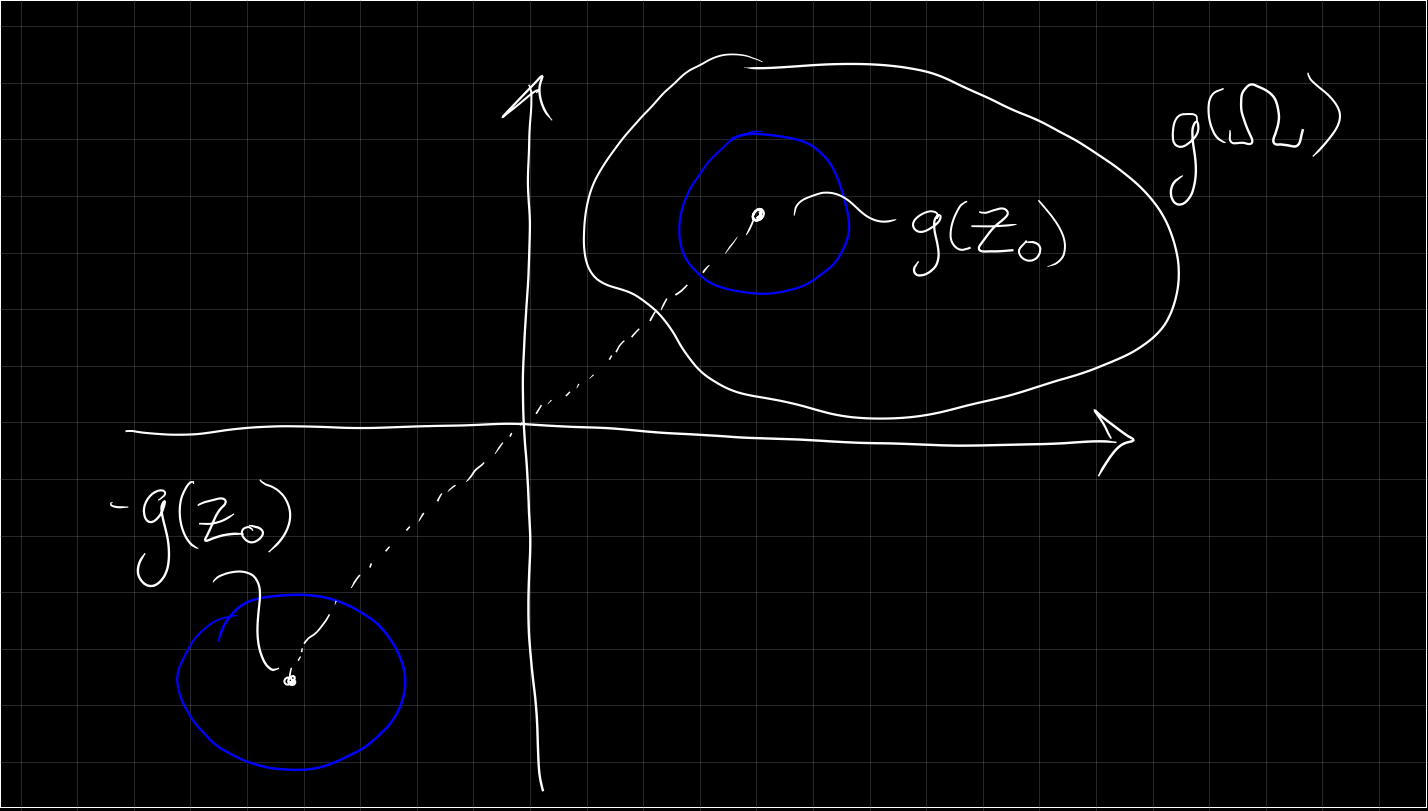
\includegraphics{figures/image_2020-04-08-14-05-50.png}\\

\begin{verbatim}
and hence $\abs{g(z) + g(z_0)} \geq r$ for all $z\in \Omega$.
Then the function $g_1(z) \definedas {\eps \over g(z) + g(z_0)}$ is holomorphic and injective in $\Omega$, for $\abs{\eps} < r$ satisfies $\abs{g_1(z)} < 1$.
So $g_1$ satisfies properties (a) and (b).

\

We now take $g_0 \definedas \psi \circ g_1$ where $\psi \in \Aut \DD$; we want $g_0(z_0) = 0$ with positive derivative.
Choosing $\alpha = g_1(z_0)$ forces $g_0(z_0) = 0$, and using the chain rule to compute the derivative explicitly shows
\begin{align*}
g_{0}^{\prime}\left(z_{0}\right)=\frac{\left|g_{1}^{\prime}\left(z_{0}\right)\right|}{1-\left|g_{1}\left(z_{0}\right)\right|^{2}}>0
.\end{align*}
\end{verbatim}

\hypertarget{friday-april-10th}{%
\section{Friday April 10th}\label{friday-april-10th}}

Continuing the proof from last time. Existence involved

\begin{itemize}
\tightlist
\item
  The square root function
\item
  Reciprocal functions
\item
  Automorphisms of the disc
\end{itemize}

\begin{description}
\tightlist
\item[Definition]
Let \(\Omega \subset \CC\) be open. A family \(\mcf(\Omega)\) of
holomorphic functions on \(\Omega\) if every sequence has a subsequence
that converges uniformly on every compact subset of \(\Omega\), where
the limit need not be in \(\mcf(\Omega)\).
\end{description}

Proving that a family of functions is normal is a consequence of

\begin{itemize}
\tightlist
\item
  Uniform boundedness
\item
  Equicontinuity
\end{itemize}

\begin{description}
\tightlist
\item[Definition]
A family \(\mcf\) is said to be uniformly bounded on compact subset iff
for each compact \(K \subset \Omega\) there exists \(B_K > 0\) such that
\begin{align*}
\abs{f(z)} \leq B_k \quad\text{for all} \quad z\in K, f\in\mcf
.\end{align*}
\item[Definition]
A family \(\mcf\) is equicontinuous if for every \(\eps > 0\) there
exists \(\delta > 0\) (not depending on the point) such that for all
\(z, w\in K\), \begin{align*}
\abs{z-w} < \delta \implies \abs{f(z) - f(w)} < \eps \quad\forall f\in\mcf
.\end{align*}
\end{description}

Examples:

\begin{enumerate}
\def\labelenumi{\arabic{enumi}.}
\tightlist
\item
  The family \(f_n: I \to \CC\) with \(\abs{f_n'} \leq M\) for some
  fixed constant is uniformly bounded and equicontinuous (by the MVT).
\item
  The family \(f_n(x) \definedas x^n\) for \(x\in I\) is uniformly
  bounded but not equicontinuous since
  \(\lim_{n\to\infty} \abs{f_n(1) - f_n(x_0)} = 1\) for any
  \(x_o \in I^\circ\).
\end{enumerate}

\begin{description}
\item[Theorem (Montel)]
Suppose \(\mcf(\Omega)\) is uniformly bounded on compact subsets, then

\begin{enumerate}
\def\labelenumi{\arabic{enumi}.}
\tightlist
\item
  \(\mcf\) is equicontinuous on every compact subset,
\item
  \(\mcf\) is a normal family.
\end{enumerate}
\end{description}

The proof of the theorem consists of two parts:

1.Apply the Cauchy integral formula and use that \(\mcf\) is comprised
of holomorphic functions.

\begin{quote}
Note the contrast to \(\RR\), where
\(f_n(x) = \sin(nx), \abs{f_n(x)} \leq 1\) is uniformly bounded but not
equicontinuous and has no convergent subsequences on \emph{any} compact
subinterval of \(I^\circ\).
\end{quote}

\begin{enumerate}
\def\labelenumi{\arabic{enumi}.}
\setcounter{enumi}{1}
\tightlist
\item
  Use the fact that uniform bounded + equicontinuous implies existence
  of convergent subsequences by Arzela-Ascoli (which uses
  diagonalization).
\end{enumerate}

\begin{quote}
Not complex-analytic, works in \(\RR\).
\end{quote}

\begin{description}
\item[Definition]
A sequence \(\theset{K_\ell}\) of compact subsets is called an
\emph{exhaustion} of \(\Omega\) iff

\begin{enumerate}
\def\labelenumi{\arabic{enumi}.}
\tightlist
\item
  \(K_\ell \subset (K_{\ell+1})^\circ\) for all \(\ell\),
\item
  Any compact \(K\subset \Omega\) is contained in some \(K_\ell\), and
  \(\union_\ell K_\ell = \Omega\)
\end{enumerate}
\item[Lemma]
Any open \(\Omega \subset \CC\) admits an exhaustion.
\item[Proof]
If \(\Omega\) is bounded, take
\(K_\ell = \theset{\dist(z, \bd \Omega) > \frac 1 \ell}\). Otherwise,
take \(\tilde K_\ell = K_\ell \intersect B_\ell(0)\).
\end{description}

\hypertarget{proof-of-montels-theorem}{%
\subsubsection{Proof of Montel's
Theorem}\label{proof-of-montels-theorem}}

Proving part 1.

Let \(K \subset \Omega\) be compact, choose \(r> 0\) such that
\(D_{3r}(z) \subset \Omega\) for all \(z\in K\),
e.g.~\(3r < \dist(K, \bd \Omega)\). Let \(z, w\in K\) with
\(\abs{z-w} < r\) and let \(\gamma = \bd D_{2r}(w)\).

Then Cauchy's integral formula yields \begin{align*}
  f(z)-f(w)=\frac{1}{2 \pi i} \int_{\gamma} f(\zeta)\left[\frac{1}{\zeta-z}-\frac{1}{\zeta-w}\right] d \zeta
.\end{align*}

Then since \(\xi \in \gamma\) and \(\abs{z-w} < r\), we have

\begin{align*}
  \left|\frac{1}{\zeta-z}-\frac{1}{\zeta-w}\right|=\frac{|z-w|}{|\zeta-z||\zeta-w|} \leq \frac{|z-w|}{r^{2}}
.\end{align*}

Letting \(B\) be the uniform bound on \(\mcf\) and using
\(\abs{\gamma} = 4\pi r\), we can apply this estimate to obtain

\begin{align*}
  |f(z)-f(w)| \leq \frac{1}{2 \pi} \frac{2 \pi r}{r^{2}} B|z-w|
.\end{align*}

Then \(f\) is uniformly Lipschitz with the constant given above, and the
family is equicontinuous.

\begin{quote}
Application: show that derivative uniformly bounded implies function
uniformly bounded by applying Cauchy's integral formula.
\end{quote}

Proving part 2.

Let \(\ts{f_n}\) be a sequence in \(\mcf\) and \(K\subset \Omega\)
compact. Choose a dense sequence \(\ts{w_j}\), and use uniform
boundedness to obtain a subsequence \(\ts{f_{n, 1} }\) such that
\(\ts{f_{n, 1}(w_1)}\) converges. Repeat these to get
\(\ts{f_{n, j}(w_j)}\) all converge, and set \(g_n = f_{n, n}\). The
claim is that equicontinuity implies \(g_n\) converges uniformly on
\(K\).

Given \(\eps>0\), choose \(\delta\) from equicontinuity and note that
\(K \subset D_\delta(w_1) \union \cdots \union D_\delta(w_J)\) for some
\(J\) by density of \(\ts{w_i}\) and compactness of \(K\). Pick
\(N \gg 0\) such that \begin{align*}
\abs{g_m(w_j) - g_n(w_j)} < \eps \forall j=1,2,\cdots, J
.\end{align*}

Then any \(z\in K\) is in some \(D_\delta(w_j)\), then \begin{align*}
\begin{aligned}
\left|g_{n}(z)-g_{m}(z)\right| \leq \left|g_{n}(z)-g_{n}\left(w_{j}\right)\right|+\left|g_{n}\left(w_{j}\right)-g_{m}\left(w_{j}\right)\right|+\left|g_{m}\left(w_{j}\right)-g_{m}(z)\right| <& 3 \epsilon
\end{aligned}
,\end{align*}

so \(\ts{g_n}\) converges uniformly on \(K\).

\hypertarget{monday-april-13th}{%
\section{Monday April 13th}\label{monday-april-13th}}

Goal: put together pieces for the Riemann mapping theorem.

Today: normal families. Recall that normal families on \(\Omega\) are
holomorphic functions for which every sequence uniformly on every
compact subset of \(\Omega\). The family is uniformly bounded iff for
every \(K\) there exists a \(B_K\) bounding \(f\) in \(K\), and is
equicontinuous iff they are continuous with a parameter \(\delta\)
uniform for the family.

We had Montel's theorem: families that are uniformly bounded on compact
subsets are equicontinuous and normal. This used Arzela-Ascoli and a
diagonalization argument.

\begin{description}
\item[Theorem (Hurwitz)]
Suppose \(g_n\) are holomorphic and nonzero on \(\Omega\), then if
\(g_n \to g\) uniformly on compact subset, then either \(g \equiv 0\) or
\(g\) is nonzero on \(\Omega\).
\item[Proof]
The limit function \(g\) is holomorphic on \(\Omega\) by the Weierstrass
theorem. If \(g\not\equiv 0\), then the zeros of \(g\) are isolated. If
\(\gamma \sim 0\) is a simply curve on which \(g\neq 0\),
\(g'_n \to g'\) and hence \(g_n' / g_n \to g'/g\) uniformly on
\(\gamma\). By the argument principle, for \(n\gg 0\) the number of
zeros of \(g_n, g\) enclosed by \(\gamma\) are equal. Since
\(g_n \neq 0\), the theorem follows.
\item[Corollary (Hurwitz)]
If \(g_n\) are holomorphic and injective, then either \(g\) is injective
or constant.
\item[Proof]
Fix \(w\in \Omega\) and apply Hurwitz to \(g - g(w)\) on
\(\Omega \setminus \theset w\).
\item[Proof (of part (B) of Riemann Mapping)]
By Montel's theorem, \(\mcf(\Omega)\) is normal since \(\abs f < 1\) for
all \(f\in \mcf\). Let \(M = \sup{g'(z_0) \suchthat g\in \mcf} \leq M\).
By definition, we can find a sequence \(g_n\) such that
\(\lim g_n'(z_0) = M\). By normality, there exists a subsequence
uniformly convergent on compact subsets to some function \(f\).

\hfill\break

In particular, \(M < \infty\) since otherwise this would yield a simple
pole for \(f\) (which is holomorphic) and \(f'(z_0) = M\). By Hurwitz,
\(f\) is either injective or constant because the subsequence is
injective. But since \(f' = M > 0\), \(f\) is not constant.

\hfill\break

Moreover, since \(f(z_0) = \lim g_n(z_0) = 0\) and \(f'(z_0) = M > 0\),
\(f\) injective implies \(f\in \mcf\). This gives the existence of
\(f\in\mcf\) such that \(g' \leq f'\) at \(z_0\) for all \(g\in \mcf\).
\item[Proof (of part (C) in Riemann Mapping)]
We want to show that \(f(\Omega) = \DD\). Toward a contradiction,
suppose not, then there exists a \(w_0 \in \DD \setminus f(\Omega)\). We
will construct a function \(g_1 \in \mcf\) with \(g_1' > f'\) at
\(z_0\), which is a contradiction.

The function
\(-\psi_{w_0}(f(z)) = {f(z) - w_0 \over 1 - \bar w_0 f(z)}: \Omega \to \DD\)
is holomorphic, injective (since all such \(\psi\) are), and
nonvanishing since \(w_0 \not\in f(\Omega)\). Thus there is a branch of
the square root for which
\(g(z) \definedas \sqrt{-\psi_{w_0}(f(z))}: \Omega \to \DD\) is
injective.

Finally, normalize \(g\) so that its derivative at \(z_0\) is positive
and real by setting \begin{align*}
g_1(z) = { \abs{g'(z_0)} \over g'(z_0)} \qty{g(z) - g(z_0) \over 1 - \bar{g(z_0)} g(z) }
.\end{align*}

Then \(g_1\) has the same properties as \(g\) with \(g_1 = 0, g_1' > 0\)
at \(z_0\). The first claim is easy to check, and the second follows
from using
\(\dd{}{z} \qty{z - \alpha \over 1 - \bar \alpha z} = {1 - \abs{alpha}^2 \over \qty{1 - \bar \alpha z}^2 }\)
and applying the chain rule.

We now compare \(f'\) and \(g'\) at \(z_0\). Note that
\(f = 0, f' > 0, g^2 = -w_0\) at \(z_0\). Take \(\dd{}{z} g^2\) to
obtain \begin{align*}
2 g(z) g^{\prime}(z)=\frac{1-\left|w_{0}\right|^{2}}{\left(1-\bar{w}_{0} f(z)\right)^{2}} \cdot f^{\prime}(z)
.\end{align*}

Evaluate at \(z=z_0\) to obtain \begin{align*}
2 g\left(z_{0}\right) g^{\prime}\left(z_{0}\right)=\left(1-\left|w_{0}\right|^{2}\right) f^{\prime}\left(z_{0}\right) \Rightarrow\left|g^{\prime}\left(z_{0}\right)\right|=\frac{1-\left|w_{0}\right|^{2}}{2\left|g\left(z_{0}\right)\right|} f^{\prime}\left(z_{0}\right)
.\end{align*}

Combining this with the previous formula obtained from the chain rule
\begin{align*}
g_{1}^{\prime}\left(z_{0}\right)=\frac{\left|g^{\prime}\left(z_{0}\right)\right|}{1-\left|g\left(z_{0}\right)\right|^{2}}=\frac{1-\left|w_{0}\right|^{2}}{2\left|g\left(z_{0}\right)\right|} \cdot \frac{f^{\prime}\left(z_{0}\right)}{1-\left|g\left(z_{0}\right)\right|^{2}} \\
&=\frac{1-\left|w_{0}\right|^{2}}{2 \sqrt{\left|w_{0}\right|}} \cdot \frac{f^{\prime}\left(z_{0}\right)}{1-\left|w_{0}\right|} \quad \text{ using } g^2(z_0) = - w_0 \\
&=\frac{1+\left|w_{0}\right|}{2 \sqrt{\left|w_{0}\right|}} f^{\prime}\left(z_{0}\right) \\
& > f^{\prime}\left(z_{0}\right)
.\end{align*}

Where we've used the Schwarz inequality, \begin{align*}
\frac{1+\left|w_{0}\right|}{2 \sqrt{\left|w_{0}\right|}}>1
.\end{align*}

But then \(g_1' > f'\), a contradiction.
\end{description}

Note that this is a long proof in the book -- seven pages!

\hypertarget{wednesday-april-15th}{%
\section{Wednesday April 15th}\label{wednesday-april-15th}}

Last time: finished proof of Riemann mapping theorem. Needed concept of
normal families, the rest was computations.

\begin{description}
\tightlist
\item[Proposition]
Suppose \(f: \Omega \to \DD\) is a holomorphic diffeomorphism. Then
\(z \to \bd \Omega \implies \abs{f(z)} \to 1\).
\item[Proof]
For each \(\eps > 0\),
\(\bar D_{1-\eps} = \theset {\abs z < 1- \eps}\subset \DD\) is compact
and \(K_\eps \definedas f\inv (\bar D_{1-\eps}) \subset \Omega\) is
compact by continuity of \(f\). If \(z\not\in K_\eps\), then
\(\abs{f(z)} > 1-\eps\) by definition.
\item[Definition]
For \(I = (a, b) \subset \RR\) an interval, a function \(f: I \to \CC\)
is real analytic iff for each \(x_0 \in I\) there exists a
\(\delta > 0\) such that in a \(\delta\) neighborhood of \(x_0\),
\(f(x) = \sum a_k(x_0) (x-x_0)^k\) is given by a convergent power
series.
\end{description}

In this case, \(a_k(x_0)\) is given by the \(k\)th Taylor coefficient.

\begin{description}
\item[Lemma]
For \(f\) real analytic, there is a neighborhood \(U\) such that ?.
\item[Proof]
Fix \(x_0 \in I\), let \(U_{x_0}\) be a disc of radius \(\delta(x_0)\)
centered at \(x_0\) in \(\CC\) such that \(f\) equals its power series
on \(D_\delta(x_0) \intersect \RR\). Set
\(F(z) = \sum a_k(x_0) (z - x_0)^k\) for \(z \in D_\delta(x_0)\). Take
\(U = \union_{x_0 \in I} D_\delta(x_0)\) Then \(F: U \to \CC\) extends
\(F_{x_0}\) for each \(x_0\), need to show it is well-defined. This
follows from Theorem 4.5, Chapter 2 -- we have two functions taking the
same values on a sequence with an accumulation point, namely their
common restrictions to \(\RR\), and the function is defined as every
accumulation point in \(\RR\).
\item[Theorem]
Assume \(\gamma: I\to \CC\) is a simple real analytic curve with
\(\gamma'(t) \neq 0\) for all \(t\) and bounds a region \(\Omega\) such
that

\begin{itemize}
\tightlist
\item
  Points to the left of \(\gamma\) are in \(\Omega\)
\item
  Points to the right of \(\gamma\) are in \(\CC \setminus \bar \Omega\)
\end{itemize}

So \(\gamma\) separates \(\CC\). Then there is a neighborhood \(V\) of
\(\gamma\) and a holomorphic extension \(F\) of \(f\) to
\(\Omega \union V \to \CC\) with \(F(\gamma) \subset \bd \DD\) and
\(F'(\gamma) \neq 0\).
\end{description}

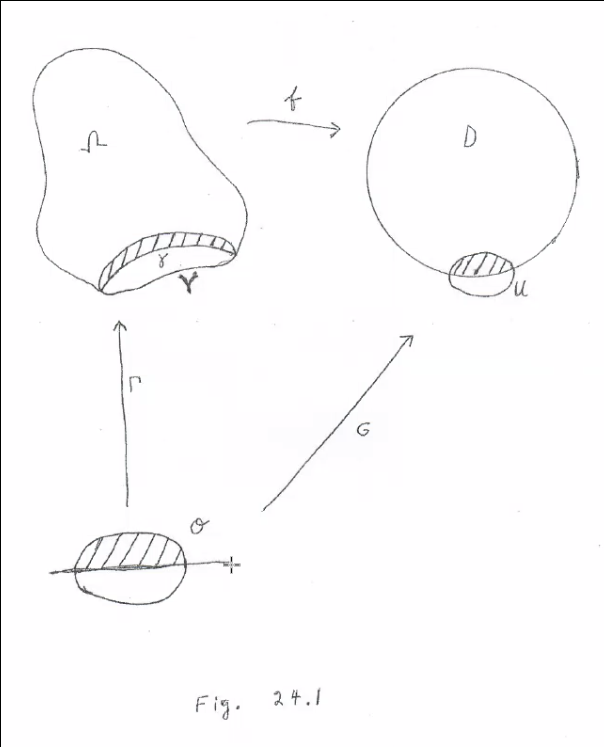
\includegraphics{figures/image_2020-04-15-14-05-21.png}

Proof

\begin{itemize}
\tightlist
\item
  Use the lemma to get a neighborhood \(O\) of \((a, b)\) in \(\CC\) and
  a univalent holomorphic extension \(\Gamma\); set \(V = \Gamma(O)\)
\item
  Assume \(O\) is symmetric about \(\RR\), say \(O^+\) is the part in
  \(\HH\).
\item
  Extend to \(G\).
\item
  ?
\end{itemize}

\begin{description}
\tightlist
\item[Theorem]
Assume \(\Omega\) is bounded and \(\bd \Omega\) is simple, closed, a
finite union of real analytic curves. Then the Riemann mapping function
\(f\) extends to a homeomorphism \(f:\bar\Omega \to \bar\DD\).
\end{description}

\hypertarget{friday-april-17th}{%
\section{Friday April 17th}\label{friday-april-17th}}

Last time: extending a real-analytic function into \(\CC\).

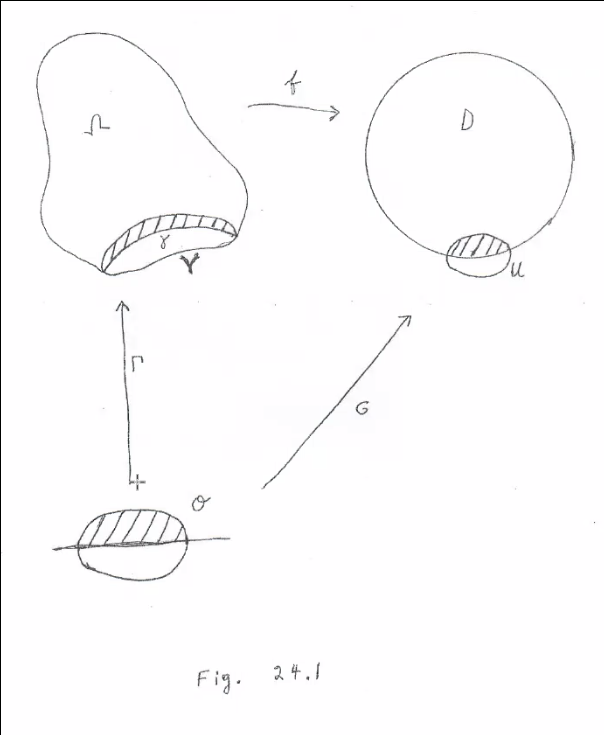
\includegraphics{figures/image_2020-04-17-13-40-45.png}\\

\begin{description}
\tightlist
\item[Theorem]
Assume \(\Omega\) is bounded and \(\bd \Omega\) is a finite union of
simple closed curves. Then the Riemann mappying function \(f\) extends
to a homeomorphism \(\bar f: \bar \Omega \to \bar \DD\).
\end{description}

Proof: Apply the previous theorem to the real analytic part of
\(\bd \Omega\), then map these diffeomorphically onto open arcs in
\(\bd \DD\). Let \(J_1, J_2\) be real analytic curves in \(\bd \Omega\)
meeting at \(p\) and let \(I_1, I_2\) denote their images in
\(\bd \DD\):

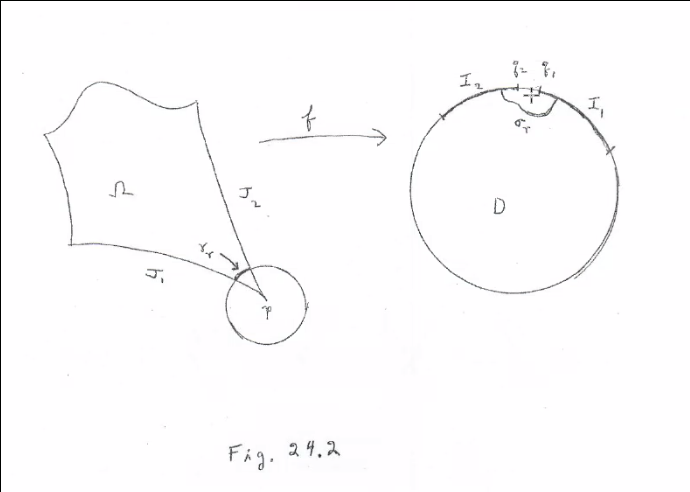
\includegraphics{figures/image_2020-04-17-13-44-28.png}\\

We want to show that \(I_1\) meets \(I_2\) and their endpoints
\(q_1, q_2\) coincide. We have \(\ell(r) = \int_{\gamma_r} \abs{f'}\),
where \(\gamma_r\) is as in the figure, and applying Cauchy-Schwarz
yields \begin{align*}
\abs{\ell(r)}^2 
&\leq_{CS} \int 1^2 \cdot \int \abs{f'}^2 \\
&\leq 2\pi r \int \abs{f'}^2 \\
\implies {\ell(r)^2 \over r} \leq 2\pi \int \abs{f'}^2
.\end{align*}

Then taking \(\ell(r) \geq \delta\) for \(\eps \leq r \leq R\) and
integrating over \(r\in (\eps, R)\) yields \begin{align*}
\delta^2 \log\qty{R \over \eps} \leq 2\pi \iint_{\Omega(\eps, R)} \abs{f'}^2 = 2 \pi ~\mathrm{Area}(f(\Omega(\eps, R))) \leq 2\pi
\end{align*} where
\(\Omega(\eps, R) = \Omega \intersect \theset{\eps \leq \abs{z-p} \leq R}\).

Since \(\log\qty{R\over \eps} \converges{\eps\to 0}\to_? 0\) there
exists a small \(r>0\) such that \(\ell(r) < \delta\). Then
\(\abs{q_1 - q_2} < \delta\), so \(q_1 = q_2\).

\begin{quote}
Note that the classification of domains is nontrivial in higher
dimension.
\end{quote}

Next goal: Picard's theorem. Best proof is Picard's original, which
comes from Ahlfors.

Recall the notion of covering maps from topology: for \(\pi: E\to X\) is
a covering map iff for every \(p\in X\) there is a \(U_x\) such that
\(\pi\inv(U) = \disjoint S_j \subset E\), where \(\pi(S_j) = U\) is a
homeomorphism.

\begin{description}
\tightlist
\item[Proposition]
If \(E, X, Y\) are connected and locally path-connected and
\(E\mapsvia{\pi} X\) is a covering map, then if \(Y\) is simply
connected then any \(f: Y\to X\) lifts to \(\tilde f: Y\to E\).
\item[Proposition]
Any continuous lift of a holomorphic map is also continuous.
\item[Proof]
Take \(q\in U, p= f(q) \in \OO\). Let \(V \ni p\) be a neighborhood such
that \(\pi\inv(V)\) satisfies the covering condition with the
projections holomorphic homeomorphisms. Then \(\tilde f(q) \in S_k\) for
some \(k\), and \(\tilde f\inv(S_k) = f\inv V = U_1\) is a neighborhood
of \(q\in U\). So the restrictions of \(\tilde f, \pi\inv \circ f\) to
\(U_q\) are equal and thus \(\tilde f\) is holomorphic on each \(U_q\).
\end{description}

Example: \(e^z\) and \(z^n\).

\begin{description}
\tightlist
\item[Proposition]
There exists a holomorphic covering map
\(\Phi: \DD \to \CC\setminus \theset{0, 1}\).
\end{description}

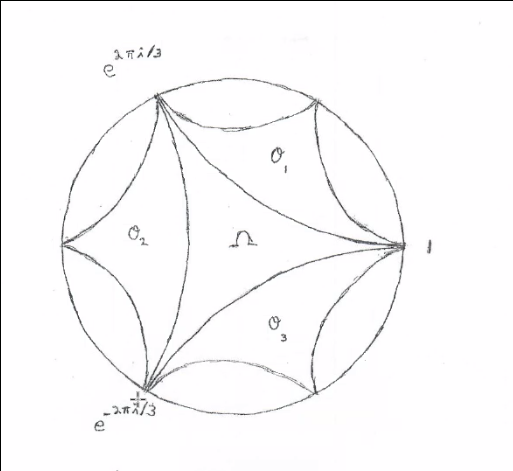
\includegraphics{figures/image_2020-04-17-14-18-10.png}

Let \(\omega = \exp({2\pi i \over 3})\), then define the LFT
\begin{align*}
\phi(z) = \omega{1 - z\over z - w^2}: \DD\to \HH
\end{align*}

which satisfies \begin{align*}
\phi(1) = 0\\
\phi(\omega) = 1
\phi(\omega^2) = \infty
.\end{align*}

and the image of the above disc is

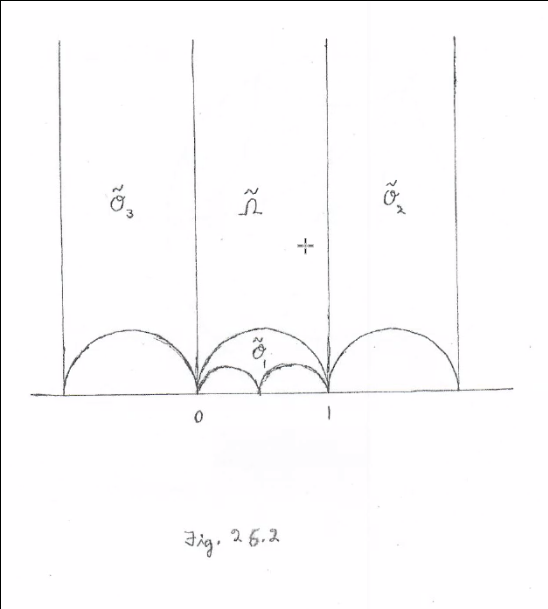
\includegraphics{figures/image_2020-04-17-14-23-25.png}\\

Then by the Riemann mapping theore, there is a holomorphic
diffeomorphism \(\psi: \Omega \to \DD\) and by the previous theorem,
this lifts to \(\bar \psi: \bar \Omega \to \bar \DD\), and \(\psi\) can
be chosen to fix \(1, \omega\). Conjugating by \(\phi\) gives a
holomorphic diffeomorphism \(\Psi: \Omega^\sharp \to \HH\) which extends
to a map \(\bd \Omega^{\sharp}\) onto \(\RR\) which fixes \(0, 1\).

Idea: continue on a fractal-like manner to cover the unit disc.

\hypertarget{monday-april-20th}{%
\section{Monday April 20th}\label{monday-april-20th}}

Goal: Picard's theorem,

\hypertarget{monday-april-27th}{%
\section{Monday April 27th}\label{monday-april-27th}}

See Simon's book and Donald for examples on definite integrals. See also
problem book, contains problems from many qual areas, although these are
more difficult.

Springer link, Ponnusamy, complex variables and applications

Stein, page 79, example 2

\newpage

\newpage
\section{Indices}
\listoftodos[List of Todos]

% Hook into amsthm environments to list them.
\renewcommand{\listtheoremname}{Definitions}
\listoftheorems[ignoreall,show={definition}, numwidth=3.5em]

\renewcommand{\listtheoremname}{Theorems}
\listoftheorems[ignoreall,show={theorem,proposition}, numwidth=3.5em]

\renewcommand{\listtheoremname}{Exercises}
\listoftheorems[ignoreall,show={exercise}, numwidth=3.5em]

\listoffigures


\printbibliography[title=Bibliography]


\end{document}
